%!TEX encoding = UTF-8 Unicode
%!TEX program = xelatex

\documentclass[master,twoside,openright]{ustcthesis}
% bachelor|master|doctor [professional] [english] [pdf] [authoryear|numebers]
\usepackage{url}
\usepackage{hyperref}
\usepackage{subfigure}
\usepackage{setspace}
\usepackage{caption}
\usepackage{ustcextra}
\graphicspath{{figures/}}

\title{Android平台的CNN模型\\能效优化问题研究}
\author{王震}
\major{计算机系统结构}
\supervisor{周学海\ 教授}
\cosupervisor{李曦\ 副教授}
% \date{二〇一七年五月一日}    % 注释掉则为今日
% \professionaltype{专业学位类型}
% \secrettext{机密\quad 小于等于20年}    % 内部|秘密|机密,注释本行则不保密

\entitle{Research about Energy Efficiency Optimization of CNN Models on Android Platform}
\enauthor{Zhen Wang}
\enmajor{Computer Architecture}
\ensupervisor{Prof. Xuehai Zhou}
\encosupervisor{Assoc. Prof. Xi Li}
% \endate{May 1, 2017}    % today if commented
% \enprofessionaltype{Professional degree type}
% \ensecrettext{Confidential\quad Less than or equal to 20 years}
% Internal|Secret|Confidential

\begin{document}

\maketitle

% 本科论文:
%   frontmatter: 致谢、目录、中文摘要、英文摘要
%   mainmatter: 正文章节、参考文献
%   appendix: 附录
%
% 硕博论文:
%   frontmatter: 中文摘要、英文摘要、目录、符号说明
%   mainmatter: 正文、参考文献
%   appendix: 附录
%   backmatter: 致谢、发表论文

\frontmatter
%!TEX root =  ../main.tex

\begin{abstract}
近年来,卷积神经网络(CNNs)因其高推断精度和强自适应性而被广泛应用于各种领域,例如:计算机视觉、语音识别等。另一方面,移动手机当前已经成为人类日常生活中的随身携带之物,并且每天都产生着大量与人类相关的传感数据。为了让手机更加智能地服务于人类,许多工程项目也尝试着在移动端利用卷积神经网络处理这些传感数据。然而,由于受到当前移动平台的资源限制(内存、计算能力、电池容量等),基于CNN模型的应用在手机移动平台上并不多见。

目前,手机上基于CNN模型的应用绝大部分都是采用“客户端-服务器”模式,但是该模式不仅强依赖于网络性能(如网络稳定性等)而且会导致用户隐私泄露。因此,许多研究学者开始探索如何在移动端离线执行卷积神经网络的前向推断过程。针对这一研究课题,本文提出了一系列优化策略并设计与实现了一套可高能效运行在Android平台的卷积神经网络推断时库。然后,本文利用该推断时库开发了一款生活日志型应用,借以探索从系统层进一步提高该类场景应用运行时能效的策略。论文的主要工作包括:

\begin{enumerate}
\item 利用预训练好的卷积神经网络模型权重在移动端重构网络,并使用OpenCL异构编程框架开发基于手机GPU加速的卷积神经网络推断时库。
\item 基于“剪枝-重训”方法对卷积神经网络模型进行压缩,并在CNN推断时库中引入稀疏矩阵向量乘(SpMV)使得运行时库支持经压缩处理的稀疏CNN模型。
\item 为了充分利用当前以及未来移动设备SoC所提供的异构计算能力,本文提出了一种使用移动平台异构设备处理器并行执行CNN推断的能效优化策略。该策略可根据目标平台所配备异构处理器间的能效差异自适应地寻找一个可高能效并行执行CNN推断的设备处理器组合。
\item 针对基于CNN模型的生活日志型应用,本文详细分析了该类应用的运行时负载特征,并进一步提出了在系统层使用动态电压频率调节技术(DVFS)提高该类应用性能或能效的方法。
\end{enumerate}

本文工作的研究意义主要包括如下三点:

\begin{enumerate}
  \item 设计与实现了一套集成离线模型压缩、异构计算任务分配等功能的移动端CNN推断时库。
  \item 提出了基于异构设备处理器高能效并行执行CNN推断的策略,该策略可在运行时主动对目标平台上的异构处理器能效进行评估。
  \item 探索了从系统层使用DVFS技术优化基于CNN模型移动端智能应用能效的策略。
\end{enumerate}


\keywords{卷积神经网络;移动平台;能效;异构计算;权值压缩;系统层优化}
\end{abstract}

\cleardoublepage

\begin{enabstract}
In recent years, Convolutional Neural Networks (CNNs) have been widely used in various domains, such as computer vision and speech recognition because of their high accuracy and strong self-adaptiveness. On the other hand, mobile phones have become carry-ons to human beings, and generate a large number of sensor data every day. In order to make mobile phones serve people more intelligently, many engineering projects also try to use CNNs to process these sensor data on the mobile phone. However, due to resource limitations (memory, computing power, battery capacity, etc.) of current mobile platforms, CNN-based mobile applications have not become mainstream on mobile platforms.

Currently, most CNN-based mobile applications adopt the client-server computing paradigm. But this paradigm not only depends on network performance (such as network stability) but also leads to privacy leakage. Therefore, many researchers have begun to explore how to perform the inference process of convolutional neural networks directly on the mobile platform. For this research topic, this paper proposes a series of optimization strategies and designs a CNN inference library, which can run on the Android platform in an energy efficient way. Then, this paper uses the inference library to develop a life-logging application to explore ways to further improve the energy efficiency of such applications. In summary, our main contributions of this paper include:

\begin{enumerate}
  \item Reconstructing the convolutional neural network on the mobile phone by pre-trained weights. Using the mobile GPU acceleration by the OpenCL framework to develop a CNN inference library.
  \item Using the pruning-retraining loop to compress CNN models. Introducing Sparse Matrix-Vector Multiplication (SpMV) into the CNN inference library to enable the runtime library to support the compressed sparse CNN model.
  \item To take full advantage of the heterogeneous computing environment provided by current and future mobile device SoCs, this paper proposes an optimization strategy which can use heterogeneous device processors to execute the CNN inference. Based on the energy efficiency difference among heterogeneous processors equipped on the target mobile platform, this strategy can adaptively find an energy efficient device processor combination to execute the CNN inference in parallel.
  \item This paper analyzes the runtime load of the CNN-based life-logging application in detail and further proposes the method of using Dynamic Voltage and Frequency Scaling (DVFS) to improve the CNN-based application performance or energy efficiency in system level.
\end{enumerate}

The research significance of this paper is described as follows:

\begin{enumerate}
  \item Designing and implementing a mobile CNN inference library that integrates functions such as model compression and heterogeneous computing task assignment.
  \item Proposing a strategy for parallel execution of CNN inference based on heterogeneous device processors. This strategy can automatically evaluate the energy efficiency of heterogeneous processors on a target platform at runtime.
  \item Exploring strategies of using DVFS to improve the CNN-based smart application energy efficiency in system level.
\end{enumerate}

\enkeywords{CNNs; Mobile platform; Energy efficiency; Heterogeneous computing; Weights compression; System-level optimization}
\end{enabstract} 
\tableofcontents
\listoffigures
\listoftables
\listofalgorithms
% \input{chapters/0.notation}

\mainmatter
\chapter{绪论}

\section{引言}
随着深度学习领域不断取得突破性的进展,基于深度学习算法的手机移动应用也如雨后春笋般发展起来。智能手机已经在逐渐改变人们的生活方式,几乎每部手机都集成着若干功能各异的传感器,这些传感器每天都在采集着与使用者相关的数据,而深度学习算法无疑是处理这些数据的最佳工具。然而,由于当前嵌入式平台的资源限制(内存、计算能力、电池容量等),基于深度学习算法的应用并没有在手机移动应用市场中成为主流。

虽然深度学习模型对硬件资源的苛刻需求阻碍了它向手机移动平台的“进军”,但是其带来的好处仍然诱惑着人们在物联网和移动硬件上采用它。目前,手机上基于深度学习模型的应用(如,图像识别、语音识别)绝大部分都是基于云端服务的,即手机端采集所需的传感数据并通过网络将数据上传到云端服务器,云端服务器在获得的数据后,运行深度学习算法进行推断,并将所得的推断结果再次通过网络传回至手机端。然而,这种处理方式带来了许多负面影响,主要总结如下:1)它可能会泄露用户的隐私数据,因为它需要将用户的一些敏感数据(如,图像、音频)发送到第三方服务端进行处理;2)它的推断执行时间将会与波动的、不可预测的网络质量(如,网络延迟、吞吐量)紧密挂钩。更糟糕的是,当网络条件很差甚至不可获取时,这种推断预测就不能正常工作;3)由于无线通信能量开销的存在,对于那些需长时期运行的应用(如,增强现实、认知助理等),使用云端处理推断任务也是不切实际的;4)当用户使用的是移动网络时,某些应用(如,需要发送视频流到云端进行处理)使用云端处理,将会消耗大量的流量,这是用户所无法接受的。

考虑到上述云端执行的负面影响,用户可能更希望那些基于深度学习模型的应用在手机本地就可以完成推断任务。另一方面,我们需要意识到高能效移动处理器的运算能力和结构复杂度一直处于不间断地发展中。例如,与4年前的iPhone 5S相比,2017年苹果发布的iPhone 8在CPU单核处理性能上拥有着232\%的增长,而在多核处理性能上更是提高了373\%。许多研究学者认为,在不久的将来,即使没有远程计算的辅助,手机移动端也可以胜任许多基于深度学习模型的计算任务。通过手工改造并简化深度学习模型(如卷积神经网络),在移动端本地设备上直接运行一些深度学习模型已经被证明是可行的,但是这样做不但需要大量的设计技巧,而且对于现存的大多数深度学习模型来说都是不可行的。更为重要的,正是因为深度学习模型的复杂性才使得推断准确度和鲁棒性取得了革命性的飞跃,而这才是智能移动应用所迫切需要的,所以手工简化模型的方式并非是我们的初衷。

与桌面、服务器端相比,手机移动端的不足不仅表现在较弱的处理能力上,还凸显在较小的内存容量上(如,华为Mate 9 Pro的内存容量为4G)。然而,因为深度学习模型具有结构异常复杂的特点,所以绝大部分模型都拥有着成百万上千万甚至上亿的参数(如,VGG16模型拥有1.8亿个参数)。这导致了许多深度模型并不能在手机移动端运行。而且,即使一些模型可以运行,其也会造成大量的内存能耗开销。

综上所述,采用深度学习算法处理移动传感数据并在手机端进行离线推断是未来手机移动应用发展的一种趋势。然而,为了实现这一目标,必须要对手机端深度学习模型的本地推断过程进行各种能效优化。因此,当前研究人员主要面对的挑战如下:

\begin{enumerate}
\item  如何利用当前移动设备处理器的特点及其未来的发展趋势,使得深度学习模型可以高能效地于手机端进行离线推断。
\item 受限于当前手机内存容量较小的不足,如何使得庞大的深度学习模型也可以正常地于手机端运行。
\item 在保证性能的条件下,如何根据应用场景的特点和系统层提供的信息,进一步降低上层基于深度学习模型应用的运行时功耗。
\end{enumerate}

\section{深度学习模型于移动端能效优化的研究现状}
\subsection{早期的探索与尝试}
Lane等人\cite{lane2015can}设计了一个基于移动设备CPU和DSP的低功耗深度神经网络的原型推断系统。他们利用该推断系统研究了一些典型的移动感知任务(如,行为感知),并将该推断系统与更加通用的传统辨识技术(如,SVM、GMM和决策树等)相比较。他们的发现表明推断系统中所使用的深度神经网络(DNNs)并不会给现代的移动硬件带来过度的负载压力,而且即使是一个简单的DNN模型(如,减少71倍的输入特征数),与传统的通用学习技巧相比,也可以改善推断精度。文献\cite{lane2015early}研究了一些深度学习算法(DNNs和CNNs)在按比例缩小后,于资源受限的嵌入式设备运行推断阶段时的行为和资源特征。Yanai等人\cite{yanai2016efficient}探究了适合在移动端实现的CNN结构,并提出了多可扩放的network-in-networks(NIN),即用户可以调整识别时间和识别精度的折中比。他们的研究发现BLAS库适合加速IOS系统上卷积层的快速计算,而NEON SIMD更适合在Android系统上加速卷积层的计算。
\subsection{基于模型压缩的优化}
文献\cite{denton2014exploiting}通过使用线性压缩技巧去除CNN模型中的冗余参数,有效加速了大型已训练好CNN模型的测试时,而为此只需要付出很小的性能折中。与\cite{denton2014exploiting}类似,Jaderberg等人\cite{jaderberg2014speeding}利用不同特征通道和卷积核间存在冗余的特征对卷积核进行低秩近似分解。文献\cite{lebedev2014speeding}使用非线性最小平方去计算一个四维卷积核的低秩CP-分解,即使用一些秩为1的张量之和表示该四维卷积核。Wu等人\cite{wu2016quantized}提出一个量化的卷积模型,可以在加速计算的同时降低模型的存储和内存的开销。Wang等人\cite{wang2016accelerating}提出一个基于低秩的、分组稀疏向量分解的方法对CNN模型的测试阶段进行加速。其将卷积核分解为一些小数量的低多线性秩张量之和,并用这些近似张量代替原始的卷积核进行标准回传以达到对模型的进一步微调。
\subsection{基于异构计算的优化}
为了验证使用移动端GPU做异构计算所取得的性能,Lokhmotov等人\cite{lokhmotov2016optimizing}通过在三星 Chrome-book 2平台上进行预实验来刻画AlexNet的前向传输过程。最终,他们发现带有OpenBLAS支持的Caffe\cite{jia2014caffe}要比带有ViennaCL支持的Caffe快大约4倍,比带有clBLAS支持的Caffe快大约10倍。因此,当前移动端的GPU性能较差,并且,支持OpenCL的现有并行库并没有针对移动端进行优化。DeepX是Lane等人\cite{lane2016deepx}为在移动平台上运行深度学习模型设计并实现的一个软件加速器。DeepX利用一个基于网络计算(远程处理器)和本地异构处理器的混合体(包含CPUs,GPUs,LPUs等)来降低资源的开销,并通过两个推断时资源控制算法来提升性能,即:(1)运行时层压缩(Runtime Layer Compression , RLC)和(2)深度结构分解(Deep Architecture Decomposition , DAD)。然而,DeepX主要缺点有两点:(1)运行时层压缩不仅没有减少运行时内存的开销,还加重了处理器的计算量;(2)其运行时所使用的一些决策参数来源于离线计算好的值,不能适应运行环境的变化。Huynh等人\cite{huynh2016deepsense}设计了一个基于移动GPU的深度神经网络框架DeepSense。DeepSense是基于OpenCL的,故而可以在GPU上运行各种不同的CNN模型。然而,其计算密集型的操作(如,卷积运算)主要运行在GPU上,没有充分利用CPU的多核处理能力。文献\cite{latifi2016cnndroid}呈现了一个基于GPU加速的库(CNNdroid),其主要使用了Android官方的高性能计算框架RenderScript来加速已训练CNN模型的推断过程。然而,其并没有对一些较大的模型做压缩处理,使得一些大模型不能正常运行。
\subsection{其他优化方法}
除了上述三类研究外,还有一些其他的相关研究。文献\cite{lane2015deepear,chen2014small,variani2014deep}通过按比例缩小深度模型的方法,将深度学习算法缩小后运行在手机或DSP上。使用低功耗处理器也被证明对于连续传感类型的应用特别有效,该类系统诸如Speakersense\cite{lu2011speakersense}、Dsp.ear\cite{georgiev2014dsp}等,它们在应用级进行优化以均衡主处理器和协处理器间的负载。Antoniou等人\cite{antoniou2016general}将深度卷积模型应用在智能监控系统中,分别于PC和移动设备上实现了一款可以自动检测、智能识别的在线监控系统。最后,开发深度学习领域的专用硬件是另外一个当前较为热门的研究方向,许多研究人员对此做出了贡献,如Diannao\cite{chen2014diannao}以及FPGA神经网络加速器\cite{zhang2015optimizing}等。

可以看出深度学习模型于手机移动端的应用是近两年刚刚兴起并快速升温的研究方向。然而,大量研究学者的关注点都是放在如何提高深度学习模型于移动端的运行速度,而本课题的研究重点更多的是能效的兼顾,并且更多的会考虑能耗问题。

\section{论文的主要研究工作}
本文主要针对当前已被工业界广泛应用的深度卷积神经网络模型(CNNs)进行Android平台能效优化的研究,且主要工作包含以下方面:
\begin{enumerate}
\item 分析卷积神经网络进行前向推断时所需的基本算子,并通过OpenCL异构编程框架于手机GPU上实现计算密集型的算子。离线解析Caffe、YOLO\cite{redmon2016you}和Tensorflow\cite{abadi2016tensorflow}等深度学习框架训练出来的卷积神经网络模型权重,并将这些权重保存成统一的格式,以便在手机端可以重构不同框架训练出来的CNN模型。
\item 在保证推断精度损失极少的条件下,使用“剪枝-重训”算法对预训练好的CNN模型参数进行压缩,这样不仅可以降低网络模型的存储占用,还减少了模型重构过程中的访存数量。针对剪枝得到的稀疏矩阵,使用稀疏矩阵向量乘代替内积操作,进一步降低卷积神经网络的前向推断时间。
\item 为了能够充分利用当前以及未来移动设备SoC所提供的异构计算特征,本文提出了一种简单有效的方法,使得基于CNN模型的应用在运行时可以根据其所处运行环境中CPU、GPU等异构设备处理器的推断能效差异,自适应地寻找一个高能效的本地异构处理器组合进行CNN并行推断。
\item 针对需长时期运行的CNN模型应用(Life-logging Apps),本文通过离线分析其负载特征并建立相应模型,以期在系统层预测该类应用的运行时负载。然后,结合动态电压频率调节技术(DVFS),本文探索了从系统层进一步降低该类应用运行时功耗的可能性。
\end{enumerate}

通过上述第1、2、3点优化策略,本课题预期开发出一套可以高能效运行在Android平台的CNN推断时库,并最终将其运用在一个生活日志型应用(如,智能监控系统)中以验证第4点优化策略的有效性。

\section{论文的组织结构}

本文的章节安排如下:

第1章主要讲述了深度学习模型于手机移动端应用的现状,并分析了阻碍基于深度学习模型移动应用发展的原因以及使用手机本地离线推断的必要性。接着,通过详细介绍深度学习模型于移动端进行能效优化的研究现状,引出本文的研究内容与目标。

第2章首先介绍了卷积神经网络的相关概念和组成结构,并对反向传播算法中所使用的梯度下降法和反向传播过程进行了阐述。然后,介绍了OpenCL异构编程框架的基本概念与开发优点,并给出了基于该框架的异构程序设计流程。最后,描述了本文中所采用的能效度量标准并详细介绍了本研究中所使用的实验平台。

第3章首先对卷积神经网络前向推断过程中所使用的基本算子进行了分解,并详细描述了这些算子的作用与原理。然后,分别给出了这些基本算子在手机CPU和手机GPU上的实现方法。接着,描述了基于“剪枝-重训”的权重压缩方法,并使用该方法对卷积神经网络中占存储量主要部分的全连接层权重进行了压缩。对于压缩后的网络,进一步使用稀疏矩阵向量乘(SpMV)代替密集矩阵的内积运算,并分别给出了SpMV的CPU和GPU实现。最后,基于Caffe、YOLO和Tensorflow等深度学习框架所训练的CNN模型权重,在手机端重构LeNet-5\cite{lecun1998gradient}和AlexNet\cite{krizhevsky2012imagenet}模型,并比较分析了基于手机CPU、手机GPU和基于SpMV的实现之间的能效差异。

第4章首先探讨了当前移动端SoC的发展趋势。接着,全面分析了于手机CPU和GPU上分别执行CNN前向推断时的能效,进而阐述了利用所有可获得的手机本地处理器去执行CNN前向推断并非是一种高能效的方式。本文提出一种简单有效的方法,其可以自适应地计算特定移动平台上所有可获得的本地处理器的能效,并进一步通过计算得到一个高能效的组合去执行CNN的前向推断过程。最后,本文提出一种基于不同处理器计算性能的方法为所选组合中每一个设备处理器分配计算任务。

第5章首先介绍了动态电压频率调节技术(DVFS)的相关概念,并基于第2、3、4章设计的CNN运行时库开发了一款生活日志型Android应用——智能监控系统。针对该应用,本文从系统层分析了其负载特征并建立模型对其负载进行预测,探索了利用DVFS技术进一步降低该类应用功耗的可能性。

第6章对全文进行了总结,并对论文中尚未解决的问题提供研究线索,以期在未来的工作中加以解决并完善。

\cleardoublepage 
\chapter{技术背景与实验平台}
本文主要针对Android平台上卷积神经网络的前向推断过程进行能效优化研究,故而本章首先会对研究工作中所用到的主要技术背景进行相关介绍。由于后面章节都会对不同实现方式的能效进行实验评估,故而本章最后一节详细描述了实验中所使用的平台。2.1节介绍了卷积神经网络的基本概念,并对卷积神经网络中的几个基本层进行了详细描述;2.2节简要描述了反向传播算法中涉及的梯度下降和反向传播过程;2.3节主要介绍了OpenCL异构编程框架的基本概念和三个主要开发优点,并给出了开发基于OpenCL框架的程序设计流程。2.4节给出了评估能效的一种度量标准;2.5节对实验平台进行了详细描述。

\section{卷积神经网络}
卷积神经网络是一种深度前向反馈人工神经网络,其主要用来处理格状拓扑结构的数据,如时间序列数据和图像数据等。卷积网络在实际应用中已经取得了巨大的成功,如计算机视觉领域中的图像识别、目标检测应用等。卷积神经网络中主要采用了一种名为“卷积”的数学运算,它将一些层中的通用矩阵乘法替换为卷积操作。

\begin{figure}[htbp]
    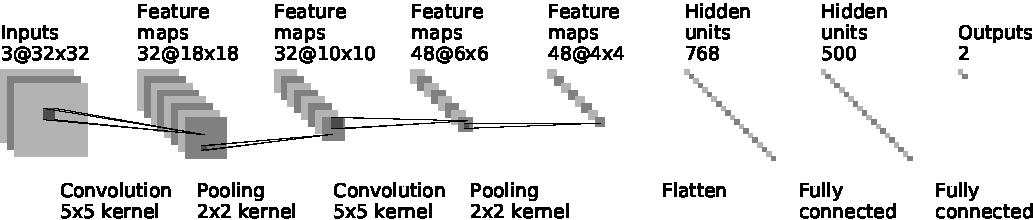
\includegraphics[width=1\textwidth]{figures/convnet_fig_cropped.pdf}
    \caption{卷积神经网络结构示意图 \cite{github.com}}\label{figure:figure1}
\end{figure}

图\ref{figure:figure1}展示了一个卷积神经网络结构案例,其由三个基本层组成,即卷积层、池化层和全连接层。简单来说,每一个卷积层通过多个卷积核将前一层低级别特征转换成高级别特征。池化层用于捕捉一些不变性,如平移、旋转或缩放后的图像经卷积层处理后的输出结果是不变的。最后,全连接层聚合提取出的高级别特征以进行进一步的分类任务。除了这三种基本层外,输入数据在经过卷积层或池化层或全连接层之后还可能再附加一层激活层,其主要使得模型具备非线性,以解决非线性分类等问题。接下来的章节将详细这些层的含义与作用。

\subsection{卷积层}
\subsubsection{卷积操作}
卷积层从字面上来看必定执行卷积操作,其作用就是通过将多个滤波器作用在输入图像上以提取不同的特征。这些滤波器被称作卷积核,且被卷积的图像叫做特征图。下面以图\ref{figure:figure2}表示的图像数据和卷积核为例详细介绍卷积操作的整个过程。

\begin{figure}[htbp]
    \begin{center}
    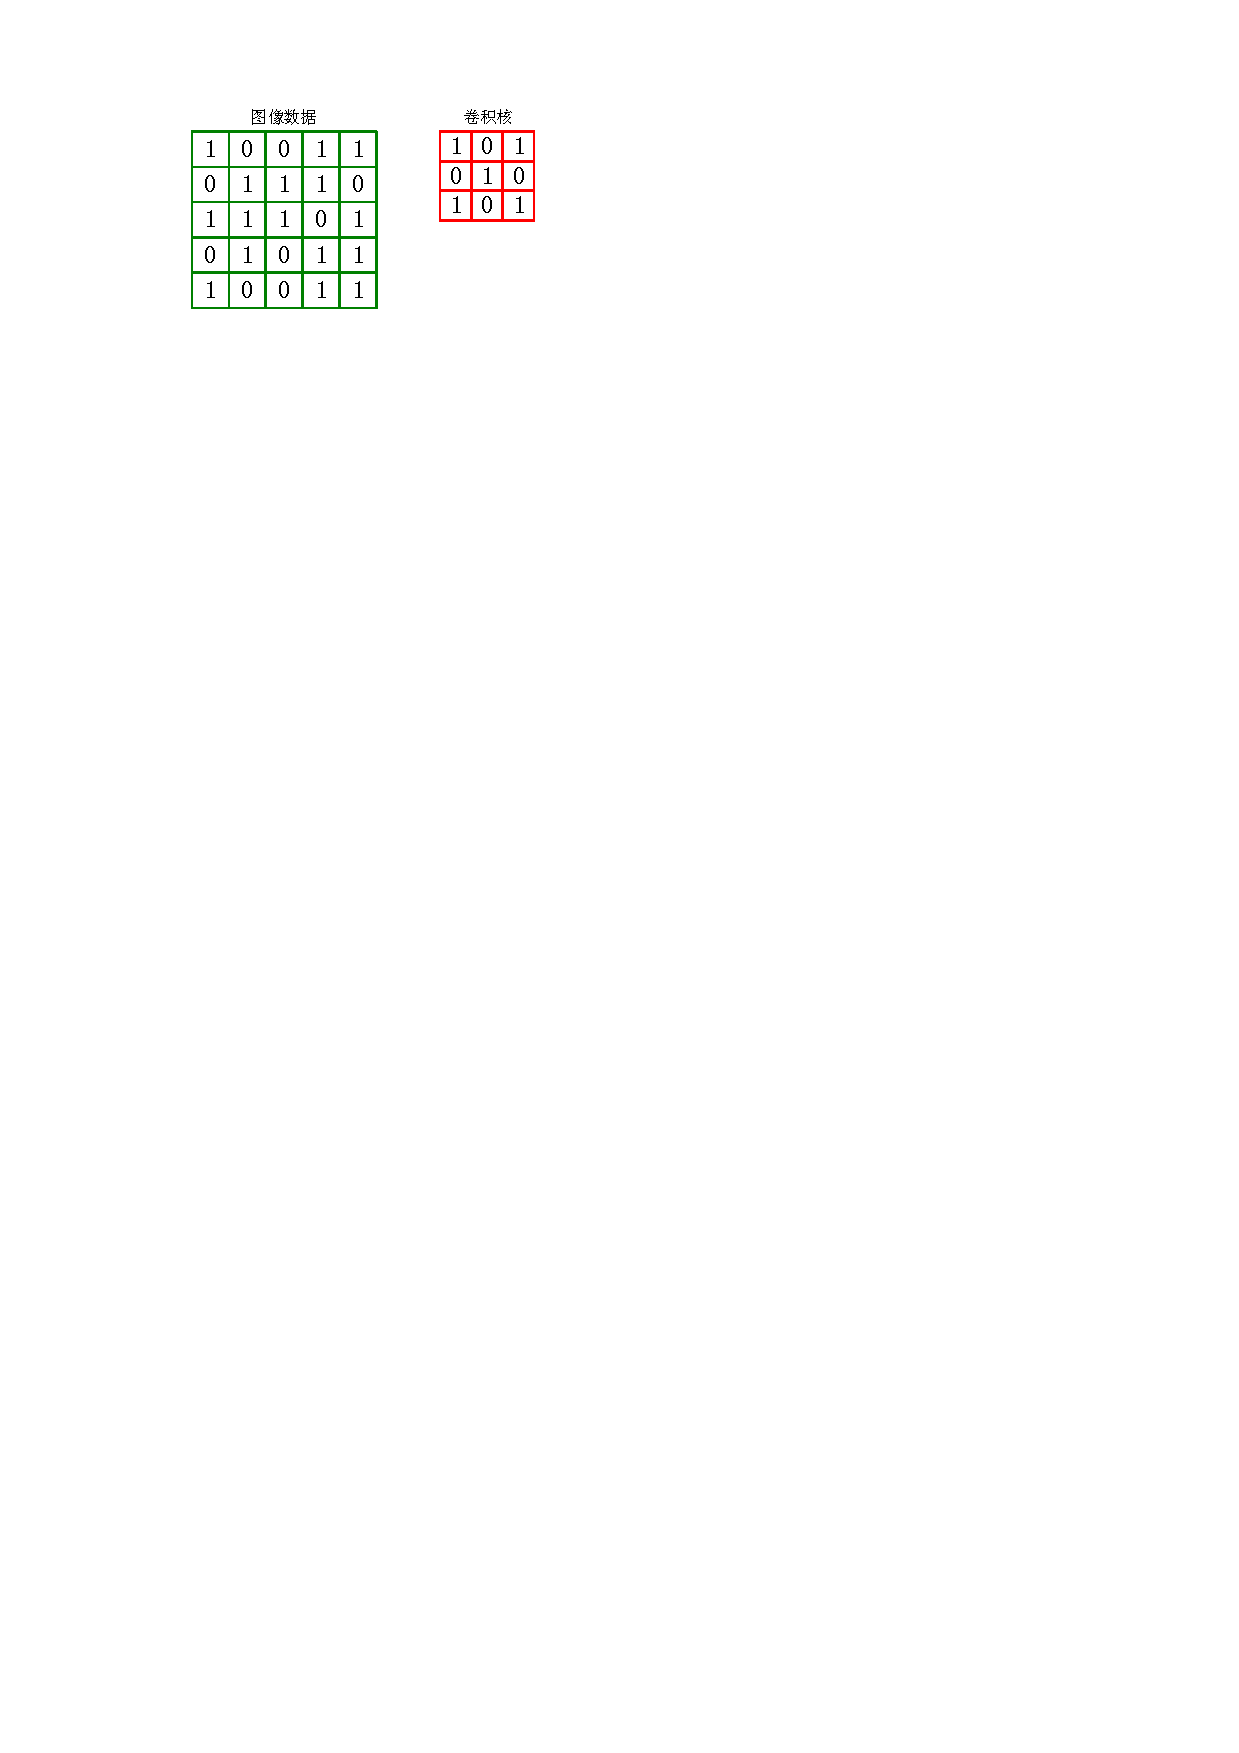
\includegraphics{figures/conv.pdf}
    \end{center}
    \caption{图像数据和卷积核}\label{figure:figure2}
\end{figure}


如图\ref{figure:figure3}所示,卷积核沿着图像从左到右、从上到下按一定步长滑过,并返回卷积核内区域图像像素值与卷积核对应值的乘积之和。通过改变卷积核的值,卷积操作就可以提取到输入图像的不同种类特征。例如,一个中间值为8而其他所有值均为-1的3$\times$3卷积核可以提取图像的边缘特征,因为它强调了颜色的差异;一个包含所有值均为0.1的3$\times$3卷积核会使得图像变得模糊不清,因为它降低了原始图像像素值。卷积神经网络的强大之处在于卷积层的卷积核权值不需要进行手工设计。卷积神经网络一经初始化后,其自身就可以通过一定的学习算法学习到合适的卷积核权重值。

\begin{figure}[htbp]
    \begin{center}
    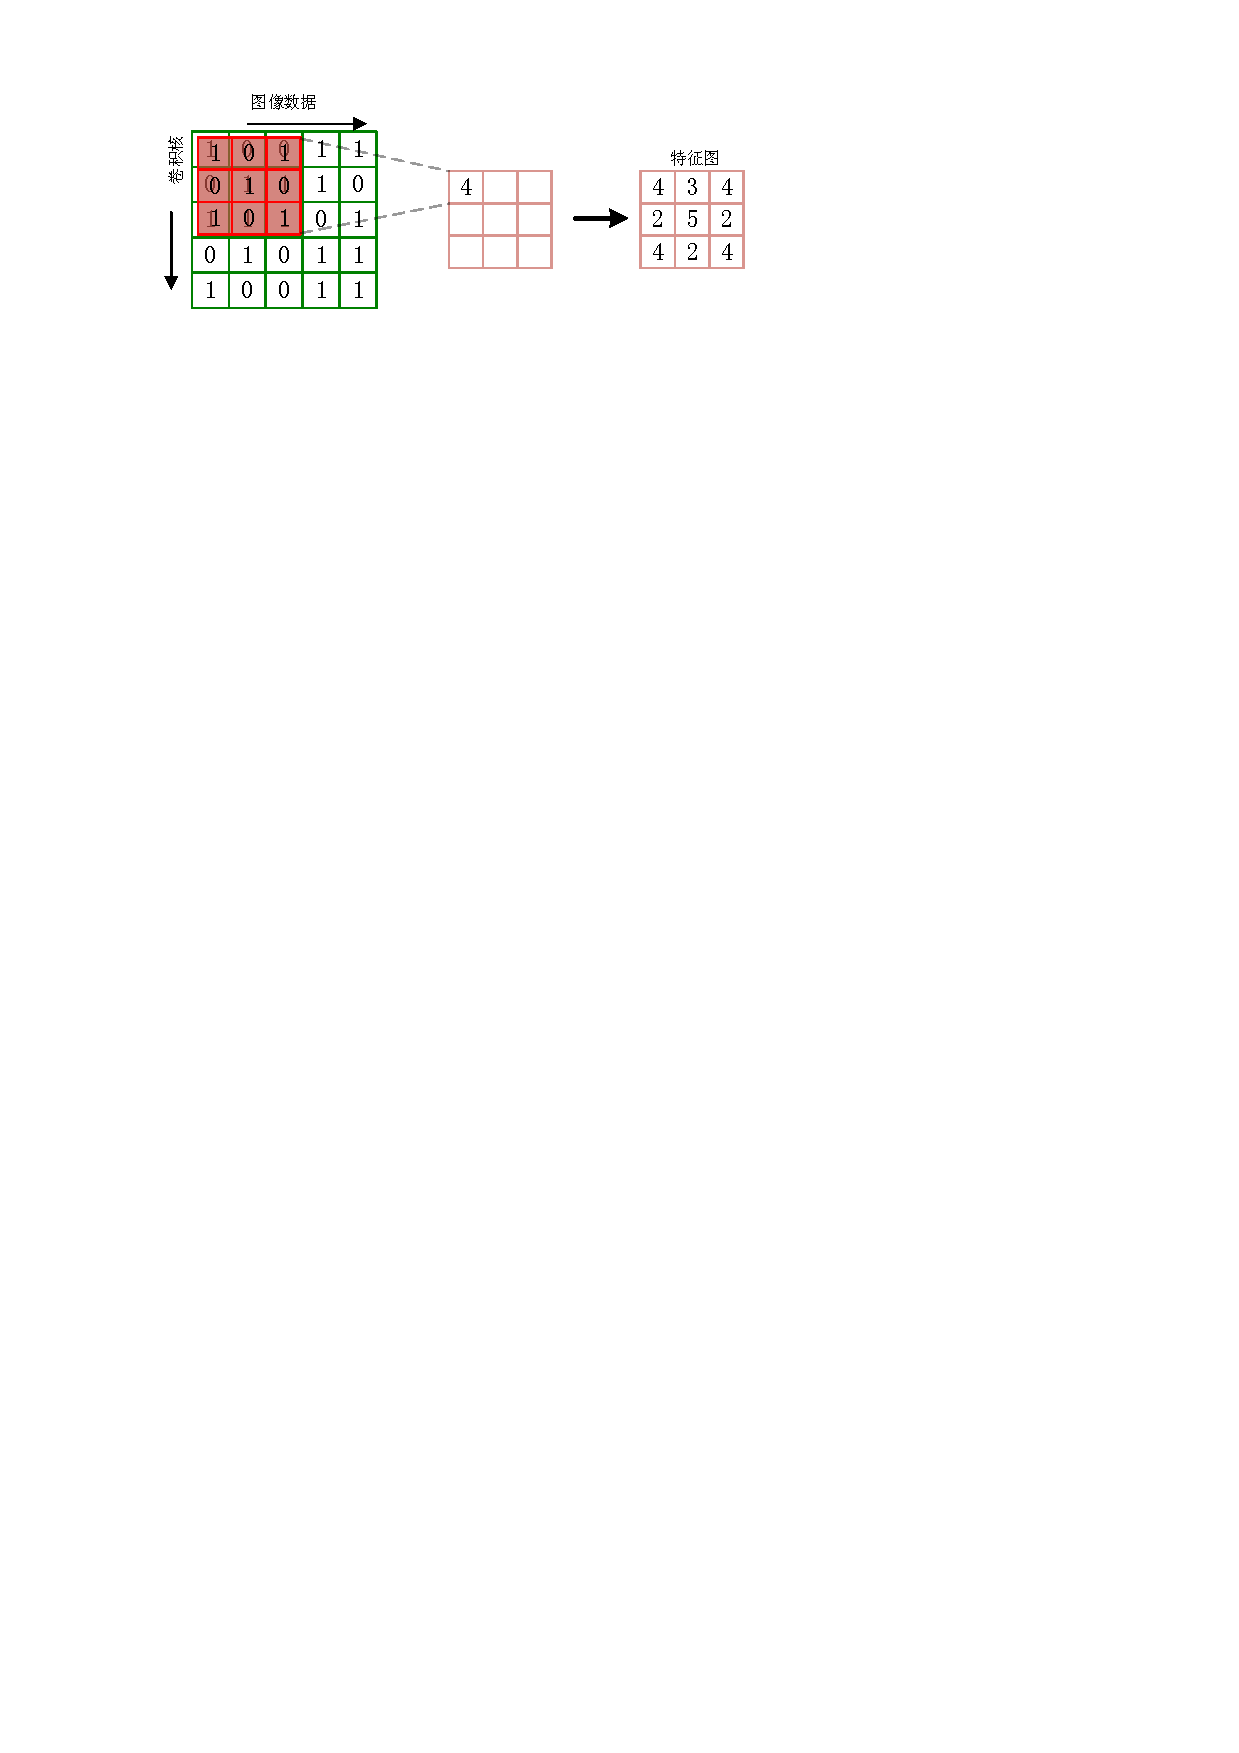
\includegraphics{figures/conv_process.pdf}
    \caption{卷积过程示意图}\label{figure:figure3}
    \end{center}
\end{figure}

\subsubsection{卷积的动机}
带有卷积层的神经网络之所以可得到很高的预测精度,是因为卷积操作利用了三个重要的思想:稀疏交互、参数共享和等变化表示。更进一步来说,卷积很好地模拟了人类视觉上的局部感受野。下面详述这三个重要思想:

\begin{itemize}
  \item \textbf{稀疏交互}:传统的神经网络层通过一个将每一输入与每一个输出相连接的矩阵参数与输入数据进行矩阵乘法运算来得到该层的输出结果。这意味着每一个输出节点与每一个输入节点都是相交互的。然而,卷积网络具有典型的稀疏交互性,也可称为稀疏连接或稀疏权重。这主要是通过将卷积核设置成远小于输入尺寸的方式实现的。例如,在处理一张图像时,输入图像可能拥有成千上百万的像素,但是我们可以使用一个每次只覆盖几十个像素点的卷积核来检测出小的、有意义的特征(如图像边沿等)。通过此种方式,网络只需要存储很少的参数,这不仅降低了模型的内存占用开销、减少了计算输出时所需的操作,还改善了模型的统计性能。
  \item  \textbf{参数共享}:这意味着对于模型中不同的功能单元可以使用相同的参数。在传统的神经网络中,计算一层的输出时权重矩阵的每一个元素只能够被使用一次,其用来与输入的一个元素相乘且不会被复用。在卷积神经网络中,卷积核的每一个元素在输入的每一个位置上都会被使用。这依赖于一个合理的假设:如果一块特征的计算在某个空间位置上是有用的,那么它在其他位置上的计算也应该是有用的。
  \item \textbf{等变化表示}:卷积操作的参数共享进一步为卷积网络附加了一个属性,即对不同变换的等变化表示。如果对一个函数的输入施加了某种变换,其输出也会响应相同的改变,那么该函数就是等变化的。特别地,一个函数$f(x)$是等变化的当且仅当$f(g(x))=g(f(x))$。对于卷积来说,如果$g$是对输入进行的任意一种平移变换,那么卷积函数对$g$来说就是等变化的。然而,卷积对于一些其他的变换(如缩放、旋转等)并不是自然等变化的,因此还需要其他的数学机制去处理这些类型的变换。
\end{itemize}

\subsection{池化层}
\label{chapter:chapter2-1-2}
与卷积层相比,池化层就相对比较简单。池化层并不直接参与训练学习,其仅仅是对卷积层传来的图像进行非线性下采样操作。最大池化(max pooling)是目前所有非线性池化操作中最为常用的。它将输入图片划分成一系列非重叠的矩形区域,对于每一个子区域将其最大值作为输出。池化层可以有效地降低数据表示的空间大小、减少网络模型的参数量和计算量,因此它也可以控制过拟合。在一个CNN模型结构中,池化层通常被周期性的插入到紧挨卷积层之后。另外,池化操作也提供了另外一种形式的平移不变性。

池化层独立地作用在输入数据的每一个通道上以调整它的空间尺寸。如图\ref{figure:figure4}所示,使用$2\times2$的滤波器在输入数据的每一个通道上沿宽和高两个方向进行步长为2的下采样操作是池化层中一个最为常用的形式,其可以丢弃$75\%$的激活结果。在该示例中,最大化操作一次作用在4个数字上,即将4个数字中的最大值作为其输出值。经池化操作后,输入数据的深度维度是保持不变的。

除了最大池化外,池化单元也可以使用其他函数,如平均池化或L2-正则池化等。平均池化在之前的研究中使用较多,但在近几年越来越多对被最大池化所代替,最大池化已被实践验证效果更佳。

\begin{figure}[htbp]
    \begin{center}
    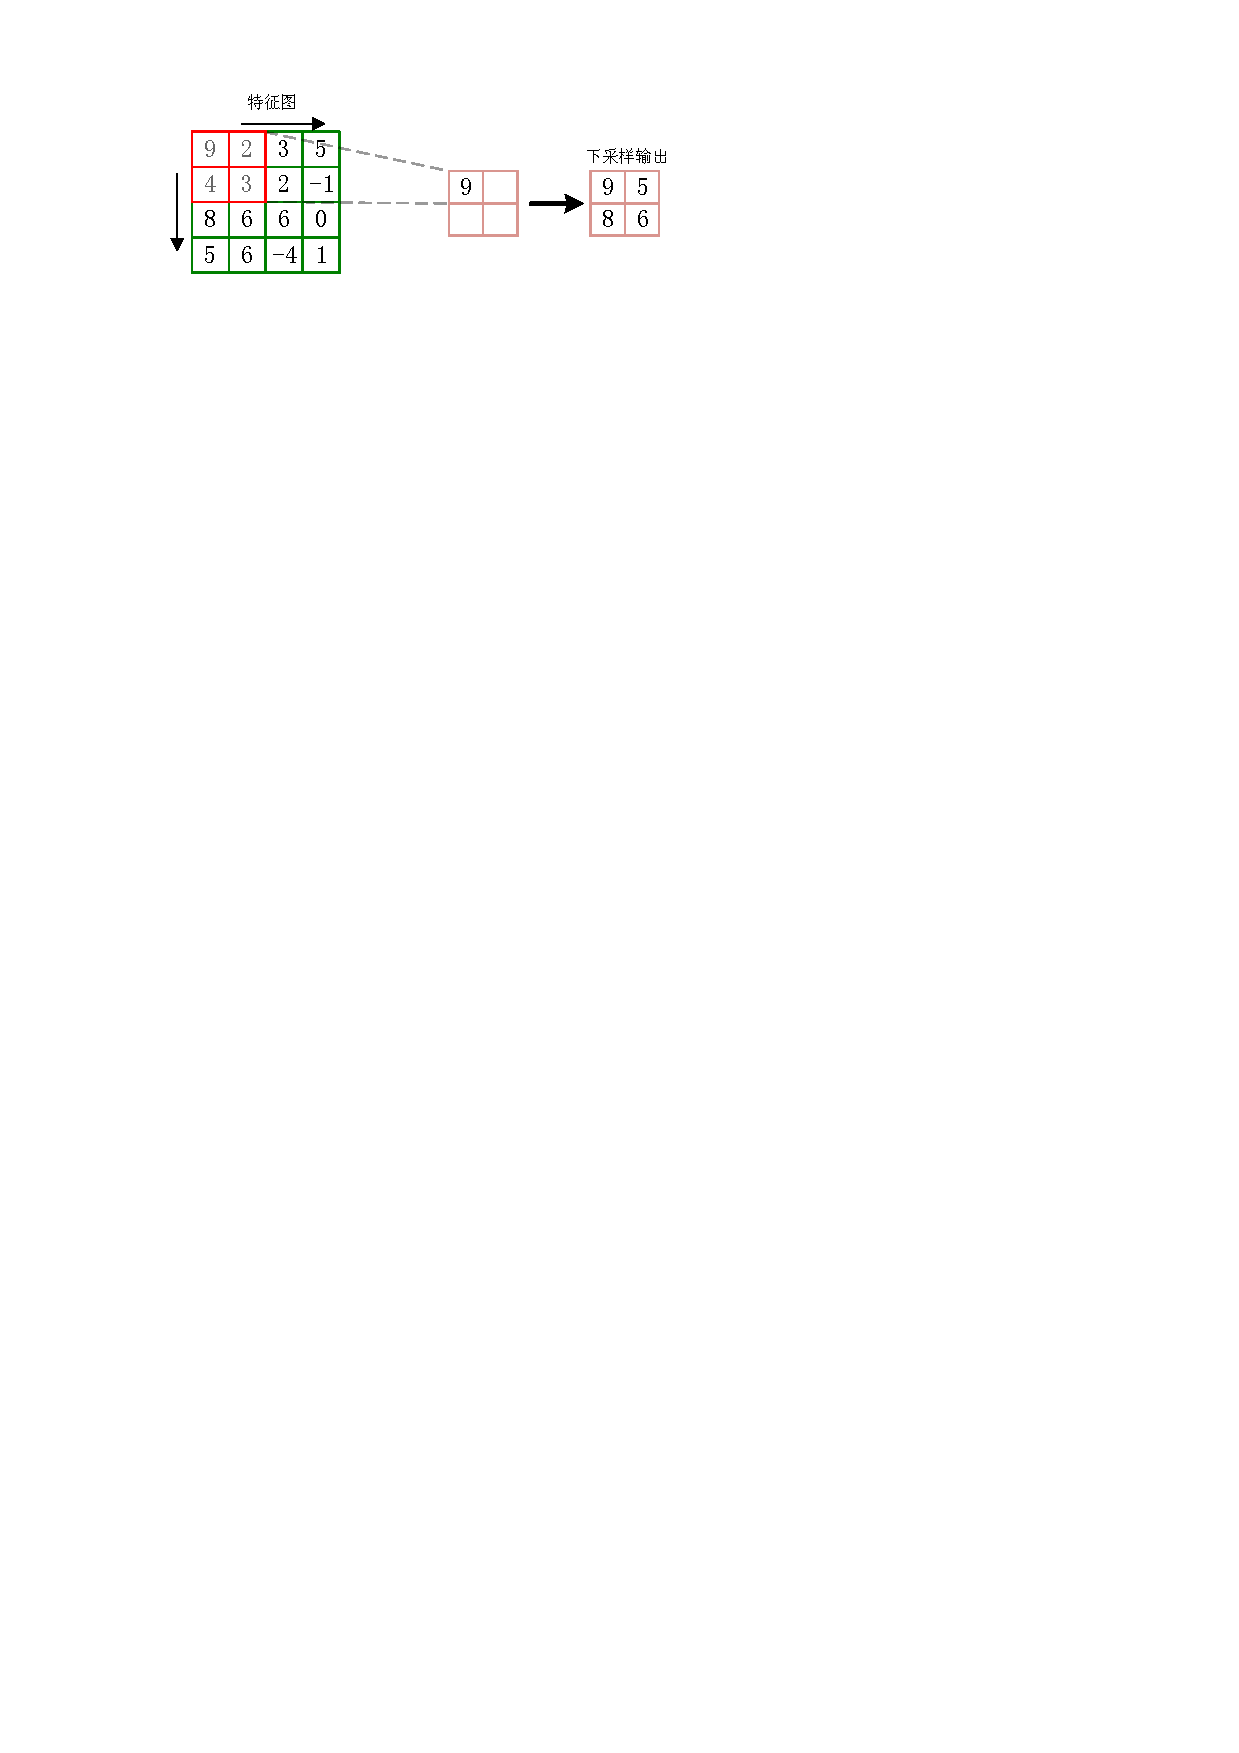
\includegraphics{figures/pool.pdf}
    \end{center}
    \caption{最大池化过程示意图}\label{figure:figure4}
\end{figure}

\subsection{全连接层}

在若干个卷积层和池化层之后,更高级别的逻辑分类是由全连接层完成的。如图\ref{figure:figure5}所示,全连接层的神经元与前一层的所有激活值进行全连接,其输出值是由输入神经元与权值矩阵进行内积操作并加上偏置矩阵(如果存在的话)而得到的。

\begin{figure}[htbp]
    \begin{center}
    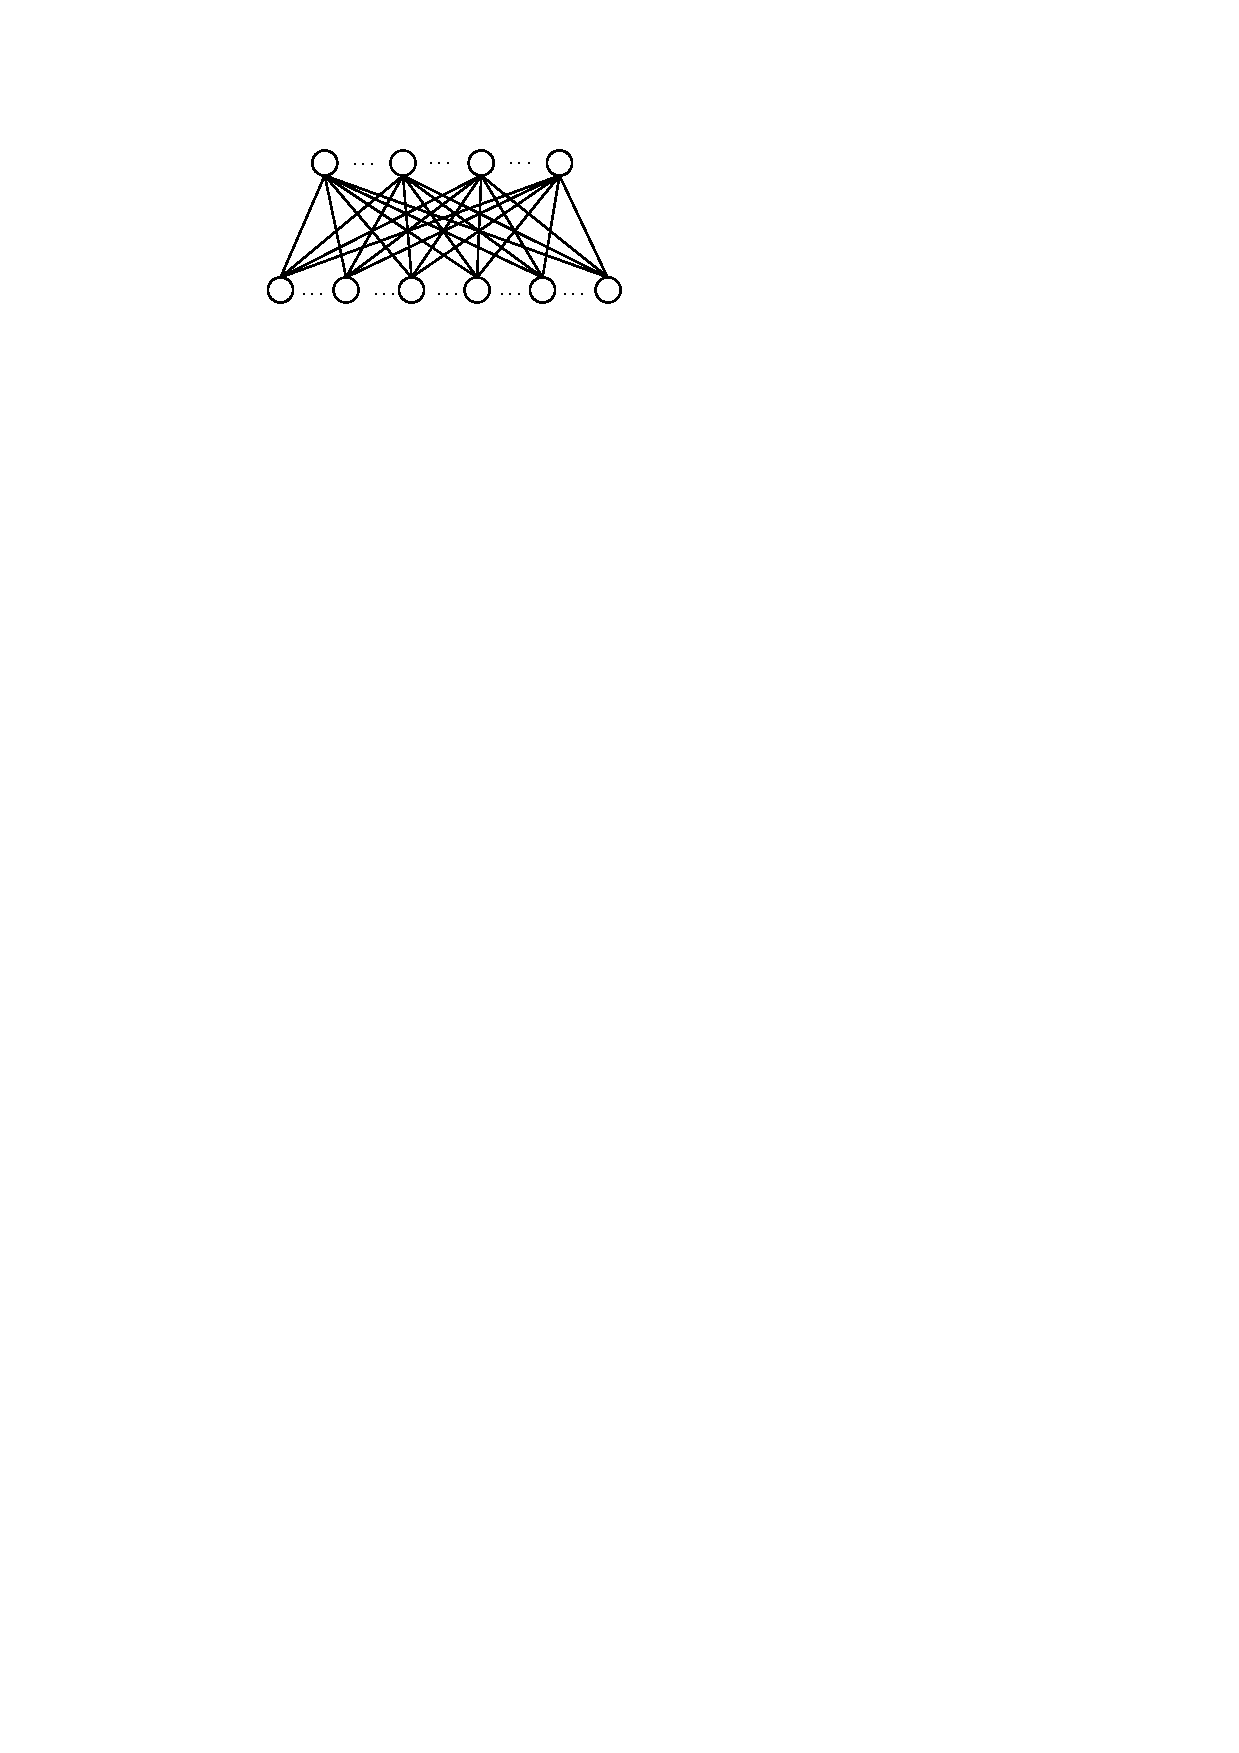
\includegraphics{figures/fc.pdf}
    \end{center}
    \caption{全连接层示意图}\label{figure:figure5}
\end{figure}

\subsection{激活层}
\label{chapter:chapter2-1-4}
激活层主要使用非线性激活函数来增强决策函数和整个网络模型的非线性属性,同时其不会影响卷积层的感受野。常用的非线性激活函数包括Relu函数($f(x)=max(0,x)$)、Sigmod函数($f(x)=(1+e^{-x})^{-1}$)和双曲正切函数($f(x)=\tanh(x)$),它们的函数图像如图\ref{figure:figure6}所示。其中,Relu函数是近年来被研究人员所青睐的非线性激活函数,因为它不仅更接近生物神经激活函数还可以在一定程度上抑制梯度消失问题的出现,而且相对于其他激活函数,使用Relu函数的模型训练速度会更快。

\begin{figure}[htbp]
    \begin{center}
    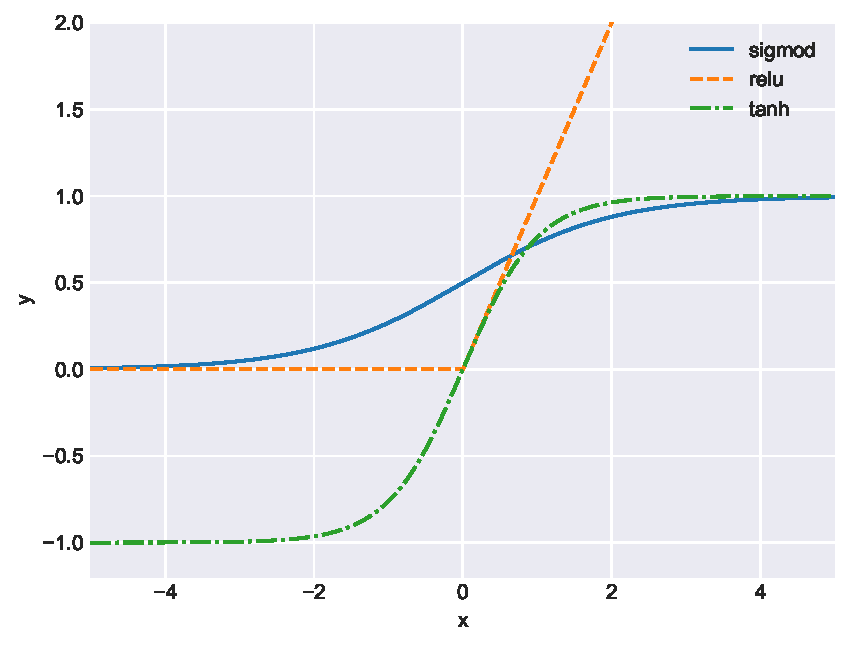
\includegraphics[height=0.4\textwidth]{figures/relu.pdf}
    \end{center}
    \caption{三种非线性激活函数}\label{figure:figure6}
\end{figure}

\section{反向传播算法}

当设计好CNN的结构,且有了训练样本,再给出损失函数的定义,接下来就可以通过反向传播算法求出CNN中的参数权重值。反向传播算法是“误差反向传播”的简称,其本质是一种利用最优化方法(如梯度下降法)训练人工神经网络的方法。该方法通过预定义的损失函数计算网络模型中所有权重的梯度,并使用这些梯度来更新权值以最小化损失函数。下面首先介绍梯度下降法,然后详细描述反向传播的计算过程。

\subsection{梯度下降}
在机器学习任务中,需要最小化损失函数$L(\theta)$,其中$\theta$是要求解的模型参数。梯度下降法常用来求解这种无约束最优化问题,它是一种迭代方法:选取初值$\theta^0$,不断迭代,更新$\theta$的值,进行损失函数的极小化。梯度下降的迭代公式为$\theta^t=\theta^{t-1}-\alpha L^{'}(\theta^{t-1})$,其详细推导过程描述如下:

\begin{itemize}
  \item 参数更新的迭代公式:$\theta^t=\theta^{t-1}+\Delta\theta$
  \item 将$L(\theta^t)$在$\theta^{t-1}$处进行一阶泰勒展开:
  $$
  L(\theta^t)=L(\theta^{t-1}+\Delta\theta) \\
  \approx L(\theta^{t-1}) + L^{'}(\theta^{t-1})\Delta\theta
  $$
  \item 要使得$L(\theta^t) < L(\theta^{t-1})$,可取:$\Delta\theta=-\alpha L^{'}(\theta^{t-1})$,则:$\theta^t=\theta^{t-1}-\alpha L^{'}(\theta^{t-1})$。此处$\alpha$是步长,一般取一个较小的数值。
\end{itemize}


\subsection{反向传播}

反向传播算法主要使用链式求导法则和梯度下降法将损失函数对于每一层的误差沿层回传以更新每层参数的权重值,其主要包括两个阶段:\textbf{传播}和\textbf{权重更新}。

每一次传播涉及如下步骤:

\begin{itemize}
  \item 通过网络进行前向传播以生成输出值。
  \item 通过损失函数计算损失(即推断误差)。
  \item 沿网络回传所有输出神经元和隐层神经元的增量,即目标值和实际输出值的差值。
\end{itemize}

每一次权值更新必须遵循如下步骤:

\begin{itemize}
  \item 将权重的输出增量和输入激活值相乘以得到权重的梯度。
  \item 一定比重($\alpha$)的权重梯度要从当前权重值中减掉。
\end{itemize}


比重$\alpha$影响着学习速度和学习质量,它也被称为学习率。学习率越高,神经网络的训练速度越快,但是较低的学习率可以使得模型训练更加精确。权重梯度的正负号表示误差是正误差还是负误差,其决定了权重变化方向(增大或减小)。从梯度下降法的推导过程可知,权重必须沿着逆梯度方向增长。上述两个阶段在整个网络模型的学习过程中将不断在不同的批次数据上重复进行直到网络达到预设的性能。

\section{OpenCL异构编程框架}

OpenCL(Open Computing Language)是一个编写跨异构平台可执行程序的编程框架,这些异构平台包括中央处理器(CPUs)、图形显示器(GPUs)、数字信号处理器(DSPs)、现场可编程门阵列(FPGAs)以及一些其他处理器或硬件加速器。OpenCL使用基于C99的编程语言为异构设备编写程序,并使用C/C++语言编写主机程序以控制设备程序在计算设备上的运行。OpenCL为基于任务并行或数据并行的并行计算提供了一个开放的标准接口,并由非盈利技术团队Khronos Group维护。OpenCL的主要优点有三个,即可移植性、标准向量处理和并行编程。

\subsection{可移植性}
Java因其“一次编写,处处运行”的理念而广受青睐,而OpenCL可能比java更具可移植性,可以说OpenCL是“一次编写,万物运行”。每一个厂商在提供OpenCL兼容设备的同时也会提供一些工具链去编译OpenCL代码以使得这些代码可以运行在其设备上。这意味着你只需要编写你的OpenCL例程一次,就可以在任何兼容OpenCL的设备上进行编译并运行,无论该设备是一个多核处理器还是一个图形显卡。这对于常规的高性能计算来说是一个极大的便利,因为在没有OpenCL之前,高性能计算程序设计人员不得不针对不同厂商的硬件设备学习该厂商指定的编程语言。

OpenCL应用针对多种设备只需编写一次,而且这些设备不需要拥有相同的体系结构或来自同一厂商。只要所有的设备是OpenCL兼容的,编写的函数就可以运行。这对于常规的C/C++编程来说是不可实现的,因为常规C/C++编程一次只能针对一种设备编写可执行程序。

\subsection{标准向量处理}

标准向量处理是OpenCL的一个巨大优点。与物理或数学上的向量含义不同,这里的向量指的是一种数据结构,其包含多个相同数据类型的元素。在进行向量计算时,对向量中每个元素的操作是在同一个时钟周期内完成的,可完成这种类型操作的处理器包括超标量处理器或向量处理器等。当然,几乎所有现代处理器都可以进行向量处理操作,但是标准C/C++并没有定义任何基本的向量数据类型。这主要是因为向量指令通常是由厂商指定的。例如,Intel处理器使用SSE扩展,英伟达设备使用PTX指令,而IBM设备依赖于AltiVec指令处理向量。这些不同的指令集几乎没有任何共性可言。

然而,程序设计人员可以利用OpenCL一次编写向量例程,并将它们运行在不同的兼容设备上。这些OpenCL程序在不同的平台上会产生不同的编译结果:英伟达的OpenCL编译器将会生成PTX指令,而IBM的编译器会将OpenCL程序编译成AltiVec指令。由此可见,如希望编写的高性能计算程序可运行在不同的平台上,使用OpenCL编码将会节约大量的时间。

\subsection{并行编程}

并行编程可将计算任务分配到不同的处理单元上以使得这些任务可以同时执行。在OpenCL术语中,这些任务被称为核函数(\emph{kernels})。一个核函数是一段特殊的函数代码,其可以被一个或多个OpenCL兼容设备执行。核函数被主机应用(\emph{host applications})发送到一个或多个选定的设备上执行。一个主机应用是使用常规C/C++语言编写的程序,其可以运行在用户使用的主机系统上。主机应用不仅可以将核函数分发到从设备(如GPUs)上,还可以让核函数直接在主机应用正在使用的CPU上运行。

主机应用使用一个被称为上下文(\emph{context})的容器管理者与其相连的从设备。图\ref{figure:figure7}显示了主机与核函数以及设备之间的交互。

\begin{figure}[htbp]
    \begin{center}
    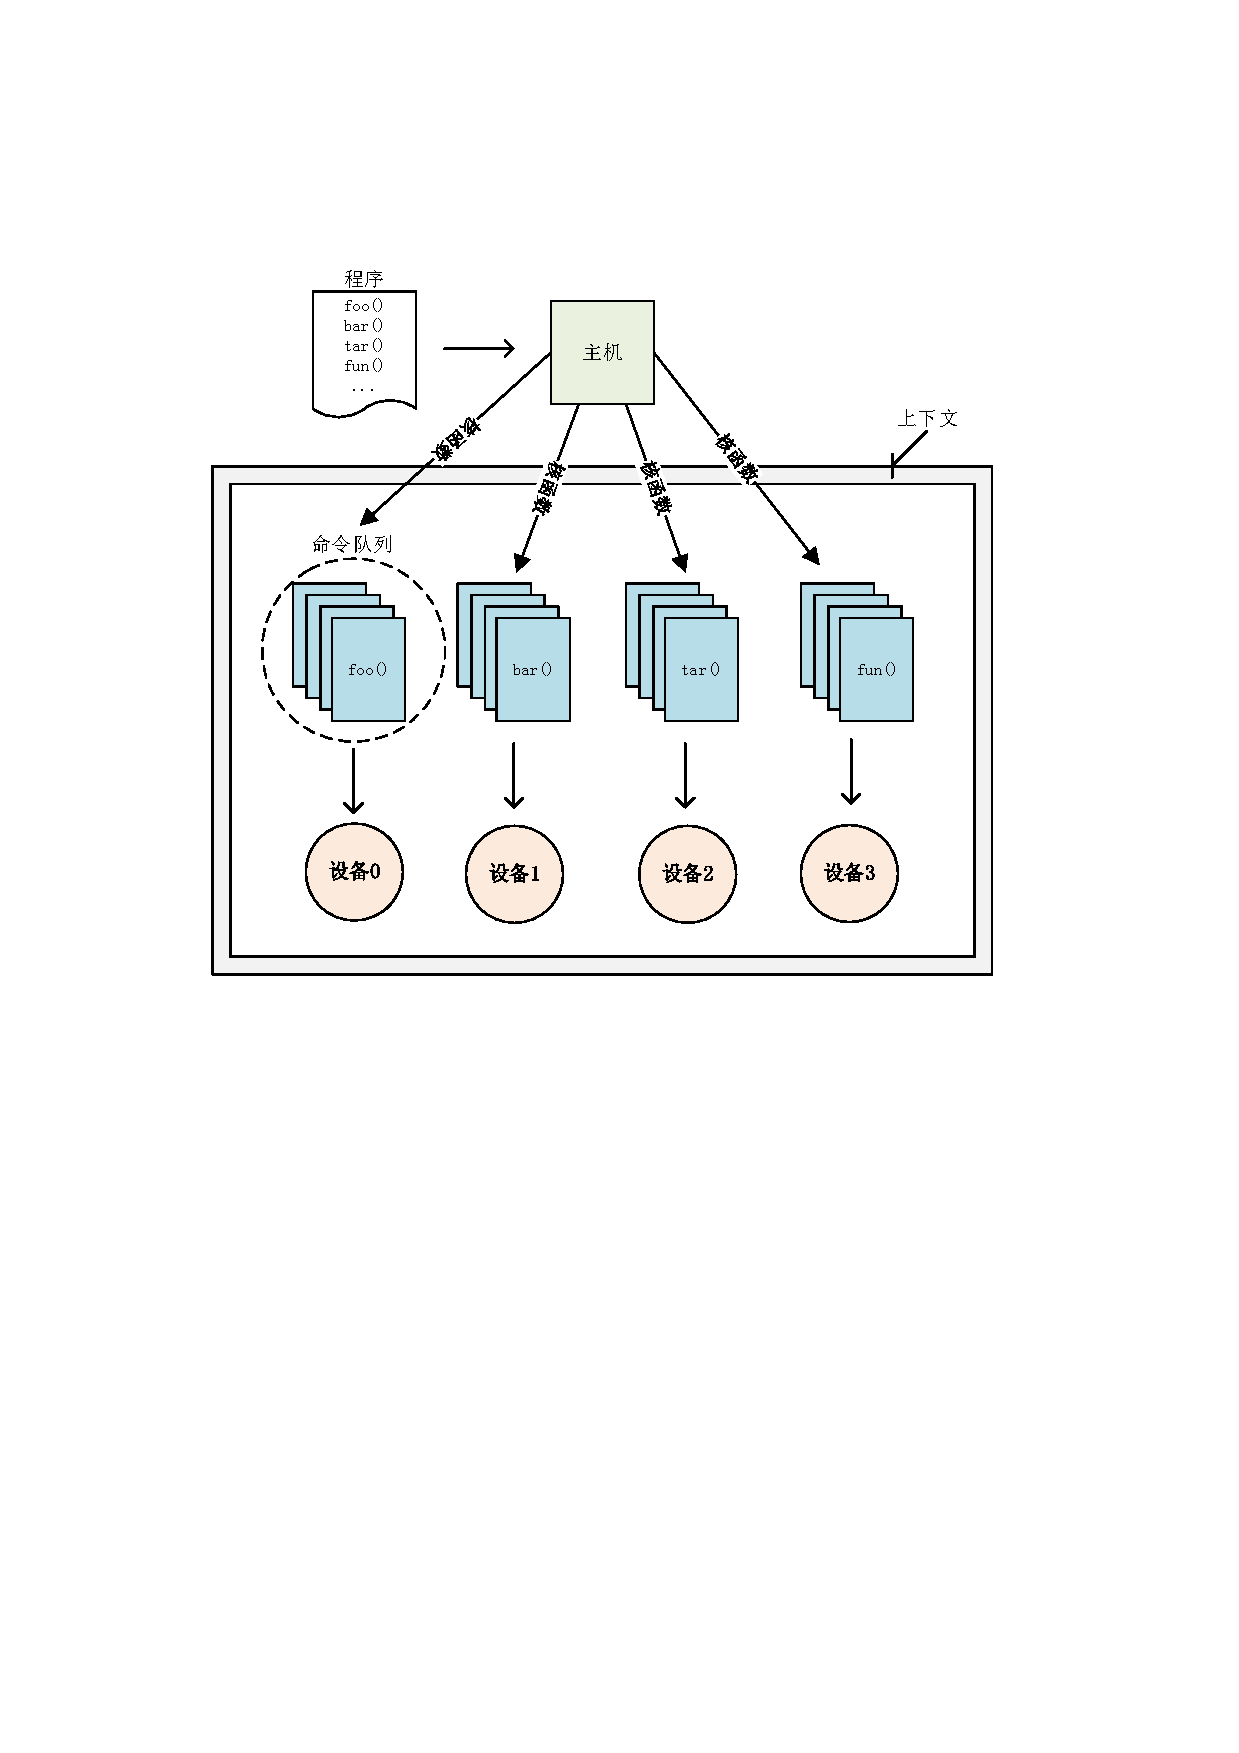
\includegraphics[width=0.8\textwidth, height=0.75\textwidth]{figures/opencl.pdf}
    \end{center}
    \caption{核函数在不同OpenCL兼容设备上的分发过程}\label{figure:figure7}
\end{figure}

为了创建一个核函数,主机从一个被称为核函数容器的程序(\emph{program})中选择一个函数。然后,主机应用设置好该核函数的参数数据并将其分派到一个被称为命令队列的结构中(\emph{command queue})。通过命令队列,主机可以告诉设备需要做的事情。当核函数入列后,设备将执行对应的函数逻辑。

一个OpenCL应用可以配置成在不同的设备上执行不同的任务,并且每一个任务也可以操作不同的数据。换言之,OpenCL提供完整的任务并行(\emph{task-parallelism})。这有别于其他许多的并行编程工具,因为它们只支持数据并行(\emph{data-parallelism})。在数据并行系统中,每一个设备接收相同的指令只是所操作的数据不同。

图\ref{figure:figure7}描述了OpenCL如何在不同的设备上完成任务并行逻辑。大多数的OpenCL设备拥有着不止一个的处理单元,这意味着在每个设备的内部还可以进行进一步的并行计算。

\subsection{OpenCL基本编程流程}

可移植性、向量处理以及并行编程使得OpenCL比常规的C/C++更加强大,但是使用OpenCL编写程序也比较复杂。在许多现实中的OpenCL应用中,程序设计者不得不创建大量的数据结构并协调好它们之间的操作。下面给出OpenCL编程的基本流程:

\begin{enumerate}
  \item 访问OpenCL平台(\emph{platform})并选择所需平台。平台是由硬件厂商提供的OpenCL框架的具体实现,不同的异构硬件生产商(如Intel、AMD、Nvidia等)可以在一个系统上分别定义自己的OpenCL框架。故而在开发OpenCL程序前,程序设计者需要查询系统中可用的OpenCL框架实现。这就需要用到\emph{platform},其对应的数据结构是cl\_platform\_id。OpenCL框架定义的\texttt{clGetPlatformIDs()} API可以用来访问并获取可用的平台,通过API \texttt{clGetPlatformInfo()}可以查看与指定平台相关的信息。
  \item 访问指定平台上的设备并选择所需设备。通过厂商提供的平台,程序设计者可以访问每一个与之相连的设备。在OpenCL应用中,设备收到的任务和数据来源于主机。在代码中,设备由cl\_device\_id数据结构表示。查询并获得设备以及查看与特定设备相关的信息可分别通过OpenCL框架定义的\texttt{clGetDeviceIDs()}和\texttt{clGetDeviceInfo()}这两个API实现。
  \item 创建上下文并通过上下文管理设备。如前所述,OpenCL的上下文主要用来标识并管理一个设备集合。目前,一个上下文只能包含来自同一平台的设备,换言之,AMD和英伟达提供的设备不能放在同一个平台上。但是,主机应用可以通过创建多个上下文来管理不同厂商提供的设备,并且同一个平台上也可以创建多个上下文。创建上下文主要由\texttt{clCreateContext()}和\texttt{clCreateContextFromType()}两个API完成。
  \item 通过上下文创建命令队列。每个命令队列与特定的某个设备一一对应,主机应用可以通过命令队列对设备进行操作,如执行核函数、设置核函数参数以及读写设备内存等。默认地,命令队列按接收顺序执行命令,但是在创建命令时也可以改变这种默认行为。\texttt{clCreateCommandQueue()} API可完成命令队列的创建工作。
  \item 使用程序(\emph{program})存储设备代码。一个程序包含了许多核函数的实现代码,由数据结构cl\_program表示。程序设计人员可以将一个文本字符串通过 \texttt{clCreateProgramWithSource()} API转换为程序这种数据结构,并可使用API \texttt{clBuildProgram()}对创建的程序进行编译。因为OpenCL使用厂商提供的编译器对设备代码进行编译,所以编译信息需要使用API \texttt{clGetProgramBuildInfo()}得到。
  \item 从程序中提取核函数(\emph{kernels})。对程序进行编译、链接后,可以使用核函数这种数据结构(cl\_kernel)将每个函数功能进行封装。核函数可以被分发到一个命令队列,进而可被与该命令队列所关联的设备执行。通过API \texttt{clCreateKernel()}可对程序中的每一个函数进行核函数封装,而API \texttt{clGetKernelInfo()}可以用来查询指定核函数的相关信息。
  \item 设置核函数参数并执行核函数。程序设计人员可以使用\texttt{clEnqueueTask()}和\texttt{clEnqueueNDRangeKernel()}这两个API将核函数入列执行,而核函数的参数可以使用API \texttt{clSetKernelArg()}进行设置。核函数入列后并不意味着马上执行,其必须要在相应的命令队列中排队等待。
  \item 读取执行结果并释放OpenCL资源。OpenCL提供了许多以clEnqueue开头的API,每一个这种函数都是通过命令队列对设备发送命令。其中,可用来读取核函数执行结果的API包括\texttt{clEnqueueReadBuffer()} 和\texttt{clEnqueueMapBuffer()}。另外,凡是通过以clCreate开头的API创建的数据结构必须通过以clRelease开头的对应API进行资源的释放。
\end{enumerate}

\section{能效度量标准}
\label{chapter:edp}

\texttt{Energy Delay Product(EDP)}是由Horowitz\cite{horowitz1994low}提出并用于评估数字电路设计领域中电路级功耗节约技术产生的能效,之后又被Brooks\cite{brooks2000power}推广使用。现在,\texttt{EDP}也经常被用来评估给定某一程序的执行能效。本文主要使用\texttt{EDP}评估一个计算过程(如CNN前向推断)使用不同优化方法所达到的能效值,它反映了该计算过程的计算延迟时间和电池电量消耗之间的折中。因此,本文中\texttt{EDP}被定义为一个计算过程的所需执行时间与所消耗电量之积,用公式形式化如下:

\begin{equation}
     \label{equation:equation1}
     \begin{aligned}
        EDP = E \times T
     \end{aligned}
\end{equation}

公式中,\texttt{E}代表能耗,\texttt{T}代表执行时间。很明显,\texttt{EDP}是一个值越小越好的度量标准。

\section{实验平台}

本文其他章节涉及到的实验都是基于ODROID-XU3\cite{hardkernel.com}和Open-Q™ 820开发套件\cite{intrinsyc.com}两个平台进行的,故而有必要在此处对它们进行详细介绍。

\subsection{ODROID-XU3}
图\ref{figure:figureodroid}所示即为Hardkernel公司生产的ODROID-XU3开发平台,其采用三星\texttt{Exynos5422}作为SoC芯片(内部集成2GB内存和\texttt{ARM Mali-T628 MP6} GPU)。实验中,ODROID-XU3运行的操作系统为Android 5.1.1版本(内核版本号为3.10.9)。\texttt{Exynos5422}的处理器使用了ARM的big.LITTLE技术,并由四个\texttt{ARM Cortex-A15}大核(频率最高可达2.0GHz)和四个\texttt{ARM Cortex-A7}小核(频率最高可达1.4GHz)组成。由于使用了\texttt{big.LITTLE™ HMP}解决方案,\texttt{Exynos5422}最多可以使用8个核去处理计算密集型的任务。\texttt{ARM Mali-T628 MP6} GPU拥有两个GPU簇,即GPU簇0包含4个\texttt{ARM Mali-T628}核而GPU簇1包含2个\texttt{ARM Mali-T628}核\cite{lokhmotov2015gemmbench}。故而,对于ODROID-XU3来说,所有可获得的本地设备处理器包括一个CPU设备和两个GPU设备\label{chapter:chapter1-1}。

\begin{figure}[htbp]
    \begin{center}
    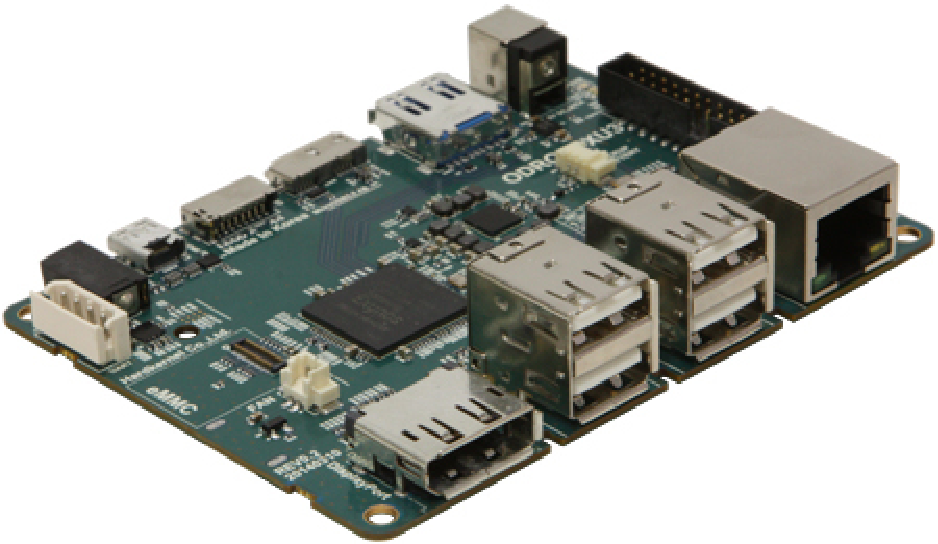
\includegraphics[width=0.4\textwidth, height=0.4\textwidth]{figures/odroid.pdf}
    \end{center}
    \caption{ODROID-XU3}\label{figure:figureodroid}
\end{figure}

为了方便研究人员测量功耗和能耗,ODROID-XU3开发平台集成了4路电流/电压传感器,它们可以独立地测量大核A15、小核A7、GPU和内存(DRAMs)的实时功耗。因为Hardkernel公司官网并未提供使用传感器测量不同部件功耗或能耗的Android APP,而本文的实验部分却都是基于Android平台的,所以本工作基于Android NDK开发了两个APP用来分别测量给定程序某段运行过程的功耗(Power Monitor)和能耗(Energy Update Service)。
\begin{itemize}
  \item \textbf{Power Monitor功能概述}:后台服务每隔50毫秒读取四路传感器的更新值,并将这些更新值追加到SD卡的Power.csv文件中;前端浮动窗每隔50毫秒进行一次界面刷新,并利用后台服务不断传回的四个传感器值绘制大核A15、小核A7、GPU和内存的实时功耗曲线。另外,可以选择关闭前端的浮动窗口以排除其在实验中的干扰。浮动窗口关闭后,后台服务会继续运行以不断更新Power.csv的文件内容。之后,可以通过离线分析Power.csv的内容来得到给定APP的功耗特征。Power Monitor的运行界面如图\ref{subfig:subfigpower}所示。
  \item \textbf{Energy Update Service功能概述}:后台服务每隔50毫秒读取四路传感器的更新值,并利用这些更新值求取自Energy Update Service应用启动以来大核A15、小核A7、GPU和内存的累积能耗。实验中使用的内核经过修改加入了两个系统调用功能:380号系统调用用于将4个最新的累积能耗值更新到指定的内核空间,而381号系统调用用于随时读取该指定内核空间的四个累积能耗值。因此,后台服务每隔50毫秒也会通过380号系统调用将4个更新后的能耗值于内核空间中进行相应更新。这样,其他的Android应用只需在待测量功耗的代码段前后打上两个桩通过两次调用381号系统调用就可以得到两个累积能耗值,两值之差即为运行该段代码所需的能耗值。Energy Update Service应用的前端浮动窗口用于实时显示四个当前累积能耗值,其也可以被关闭且不会影响后台服务的正常运行。Energy Update Service的运行界面如图\ref{subfig:subfigenergy}所示。
\end{itemize}

\begin{figure*}[htbp]
\centering
\subfigure[Power Monitor运行界面]{\label{subfig:subfigpower}
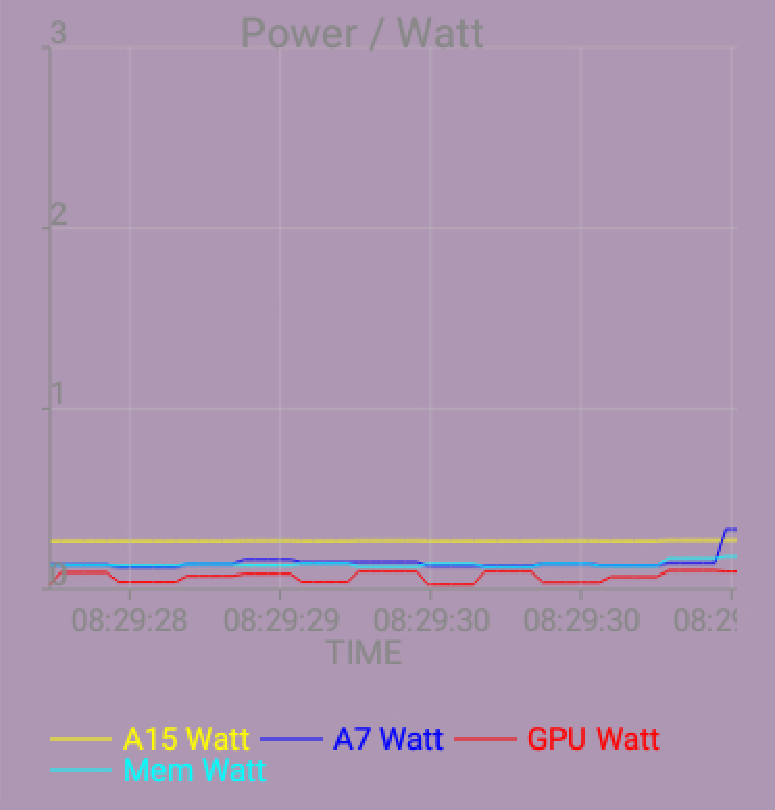
\includegraphics[scale=0.451]{figures/power.pdf}}
\subfigure[Energy Update Service运行界面]{\label{subfig:subfigenergy}
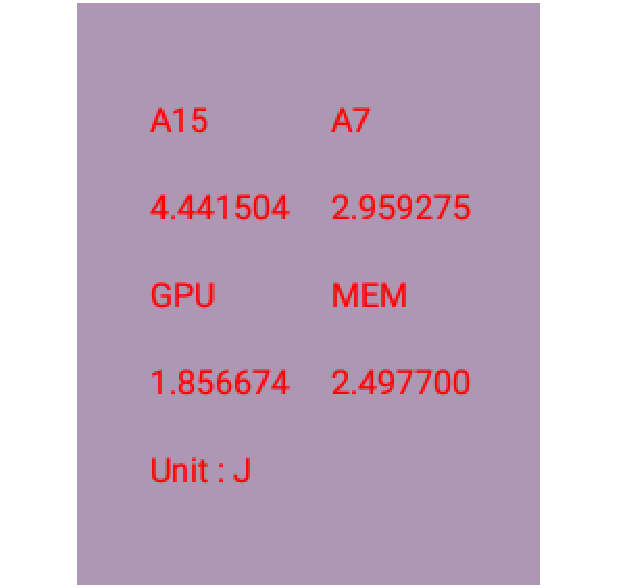
\includegraphics[scale=0.627]{figures/energy.pdf}}
\caption{功耗和能耗测量APP界面显示图}
\label{fig:subfig}
\end{figure*}

\subsection{Open-Q™ 820开发套件}

如图\ref{figure:figureopenQ}所示,Open-Q™ 820是Intrinsyc公司推出的一款基于骁龙820芯片的开发套件。骁龙820芯片不仅使用四个主频可达2.2GHz的64位元ARMv8核(\texttt{Kryo}),还配备了高通\texttt{Adreno 530} GPU和\texttt{Hexagon 680} DSP。其中,\texttt{Adreno 530} GPU虽然只包含了4个核心,但性能要比\texttt{ARM Mali-T628 MP6} GPU强大许多。另外,Open-Q™ 820还配有3GB的\texttt{LPDDR4}板载内存。实验中,Open-Q™ 820运行的Android系统版本为7.0(代号为Android N),内核版本号为3.18.31。

\begin{figure}[htbp]
    \begin{center}
    \includegraphics[width=0.4\textwidth, height=0.4\textwidth]{figures/openQ.pdf}
    \end{center}
    \caption{Open-Q™ 820开发套件}\label{figure:figureopenQ}
\end{figure}


\section{本章小结}

本章首先介绍了卷积神经网络的概念和其中一些基本层的含义与作用,这为下一章分解卷积神经网络前向推断过程中的基本算子做了准备。因为本研究工作中使用“剪枝-重训”方法对卷积神经网络的权重进行压缩,故而本章对反向传播算法中的梯度下降法以及反向传播过程进行了描述。接着,本章详细介绍了本研究中所使用的异构编程框架OpenCL的基本概念及其具备的三个主要优点,并描述了开发基于OpenCL的异构程序基本编程流程。在本章的最后,给出了评估能效的一种度量标准和实验平台的详细介绍。
\chapter{基于手机GPU加速和离线层压缩的能效优化}
\label{chapter:chapter3}
%表格模式设置左对齐:
%第一行用\multicolumn{1}{|c|}{文本内容}

本章详细分析了卷积神经网络前向推断过程中所使用基本算子,并对每一个基本算子分别给出了基于手机GPU和CPU的实现方式。基于这些基本算子,本章实现了卷积神经网络所需的层结构。然后,利用这些层结构和已训练好的CNN模型权重在手机平台上重构了LeNet-5和AlexNet,并分析比较了CPU版本和GPU版本两种实现方式的能效。最后,本章描述了基于“剪枝-重训”的权重压缩方法,并使用该方法对卷积神经网络中占存储量主要部分的全连接层权重进行了压缩。对于压缩后的CNN模型,本章进一步使用稀疏矩阵向量乘(SpMV)代替密集矩阵的内积运算,并分析了使用SpMV所带来的性能提升。

\section{CNN前向推断基本算子的分解与实现}
\label{chapter:chapter3-1}
卷积神经网络的前向推断过程主要涉及卷积层、池化层、全连接层和激活层等的前向传播,故而对CNN前向推断基本算子的分解即需剖析实现这些层所需的基本算子。下面针对每层的基本算子,详细介绍其作用机理并分析比较基于手机GPU和CPU实现版本的能效。

\subsection{全连接层基本算子}

\begin{figure}[htbp]
    \begin{center}
    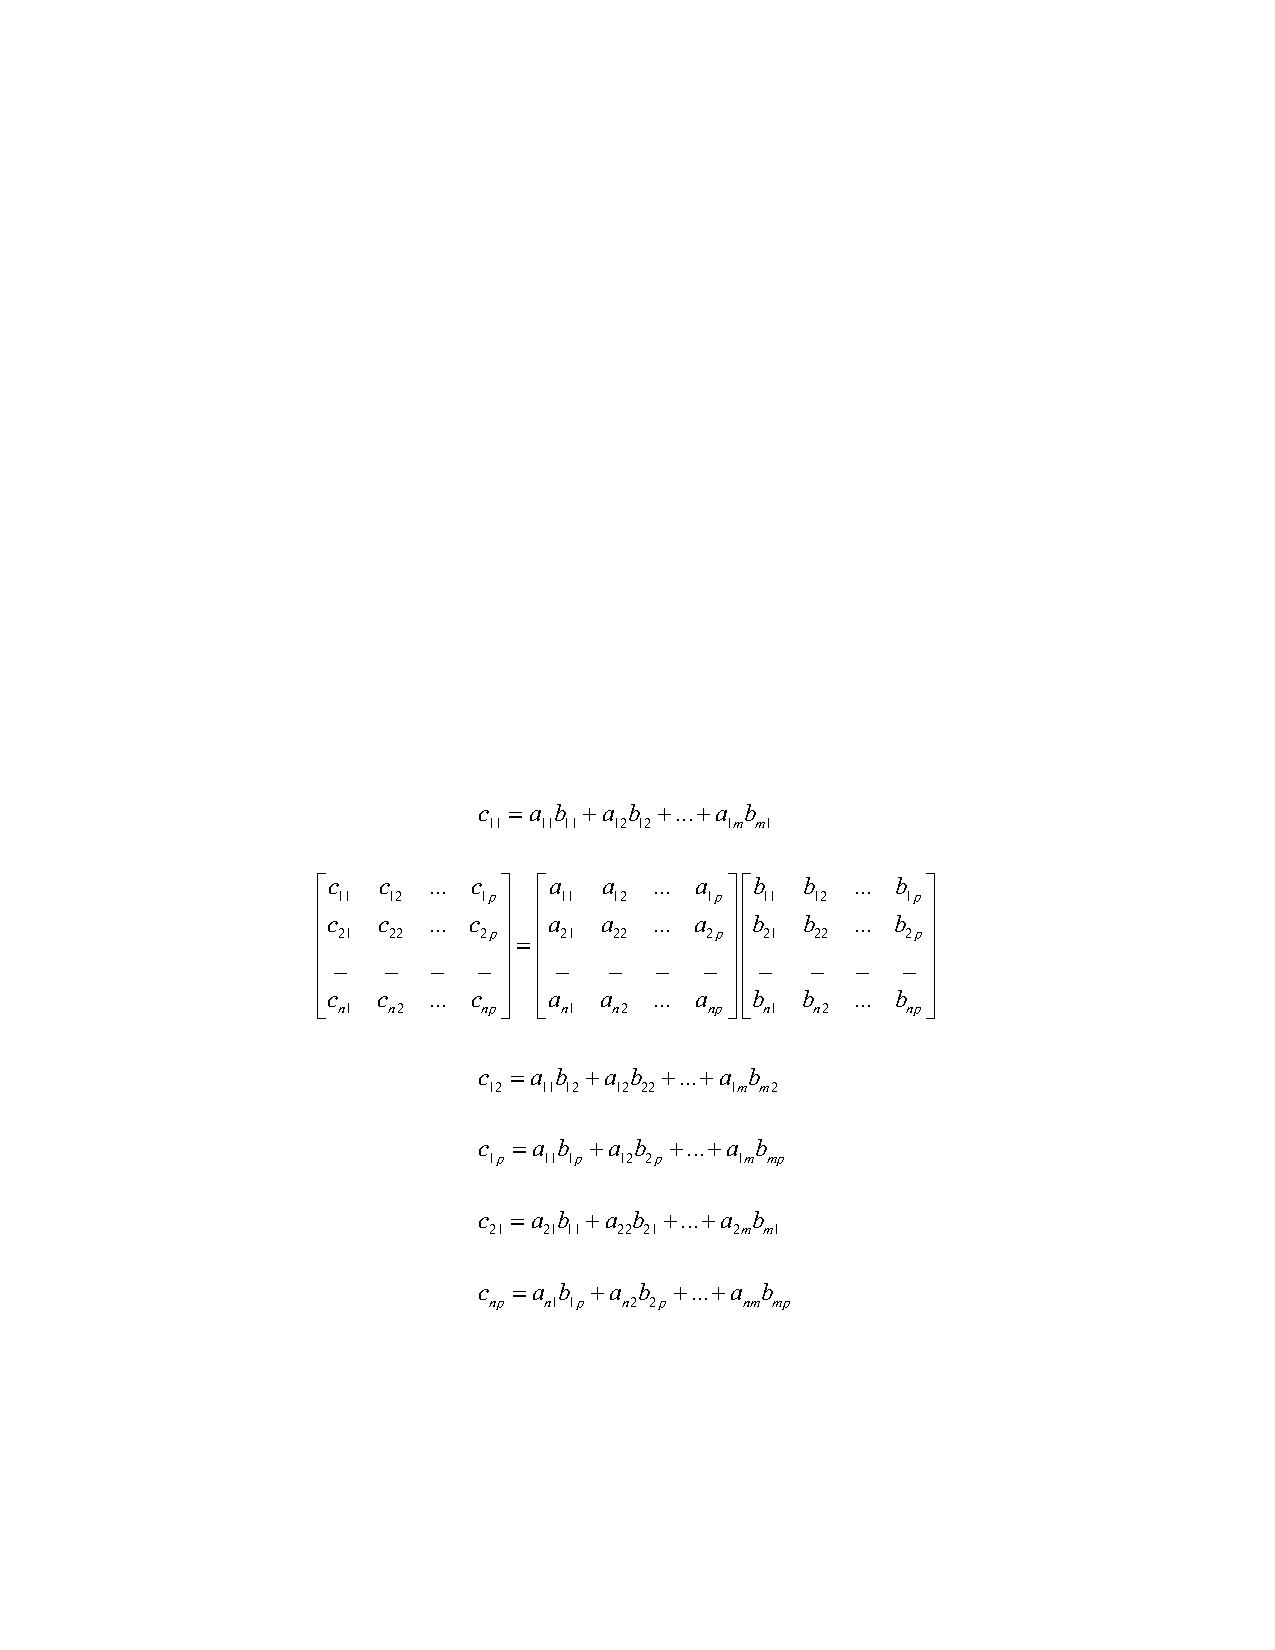
\includegraphics[height=0.5\textwidth]{figures/mat.pdf}
    \end{center}
    \caption{矩阵乘法定义}\label{figure:figure8}
\end{figure}

矩阵乘法操作是全连接层用到的主要基本算子,而在本工作的卷积层实现中其也被涉及,所以在此先介绍矩阵乘法于手机GPU和CPU上的实现。图\ref{figure:figure8}给出了矩阵乘法的定义。

根据矩阵乘法的定义可得CPU版本实现的伪代码如下:

\begin{algorithm}[htbp]
  \small
  \SetAlgoLined
  \KwData{mat\_left, row\_left, col\_left, mat\_right, row\_right, col\_right, bias, result}
    \begin{spacing}{0.9}
  \For{i in 0 ... row\_left-1}{
    \For{j in 0 ... col\_right-1}{
            res = 0\;
      \For{k in 0 ... col\_left-1}{
        res +=
        mat\_left[i * col\_left + k] *
        mat\_right[k * col\_right + j]\;
      }
    res += bias[i]\;
        result[i * col\_right + j] = res;
    }
  }
    \end{spacing}
  \caption{CPU版本矩阵乘法}
  \label{algo:algorithm1}
\end{algorithm}

基于OpenCL异构编程框架,下面给出GPU版本的矩阵乘法实现。将CPU版本中第一重和第二重循环的次数分别设置为核函数的全局工作空间大小,可将CPU版本代码直接改成GPU版本的标量形式,伪代码表示如下:

\begin{algorithm}[htbp]
  \small
  \SetAlgoLined
  \KwData{mat\_left, mat\_right, col\_left, bias, result}
    \begin{spacing}{0.9}
    初始化res的值为0\;
  i = get\_global\_id(0)\;
  j = get\_global\_id(1)\;
  col\_right = get\_global\_size(1)\;
  \For{k in 0 ... col\_left-1}{
    res += mat\_left[i * col\_left + k] * mat\_right[k * col\_right + j]\;
  }
    res += bias[i]\;
  result[i * col\_right + j] = res\;
    \end{spacing}
  \caption{GPU版本矩阵乘法(标量形式)}
  \label{algo:algorithm2}
\end{algorithm}

上述伪代码中\texttt{get\_global\_id(dim)}用于获得第\texttt{dim}维上的工作项全局ID,\texttt{get\_global\_size(dim)}用于获得第\texttt{dim}维上的全局工作项个数。GPU版本矩阵乘法的标量形式没有充分利用OpenCL的向量处理能力,这会造成一定的GPU计算性能损失。算法\ref{algo:algorithm3}给出了GPU版本矩阵乘法向量形式的核心伪代码实现。在向量形式实现中使用了\texttt{float4}向量数据类型,并通过API \texttt{dot()}完成对两个\texttt{float4}类型数据的一次内积操作。此处需要注意一点:因为对右矩阵不能使用\texttt{vload4()} API连续读4个数据,所以需要先读取所需的4个数据再将它们转换为一个\texttt{float4}向量类型,这样才能使得两个包含四个元素的向量内积操作可以在一个时钟周期内完成。

\begin{algorithm}[htbp]
  \small
  \SetAlgoLined
  \KwData{mat\_left, mat\_right, col\_left, bias, result}
    \begin{spacing}{0.9}
    初始化res的值为0\;
    remain表示核函数剩余未处理的数据量\;
    \While{remain >= 4}{
        从mat\_left中使用vload函数取出四个数据组成float4向量类型tmp1\;
        从mat\_right中取出与tmp1对应的四个数据组成float4向量类型tmp2\;
        使用dot函数计算res的当前值:res += dot(tmp1, tmp2)\;
        设置mat\_left和mat\_right的下标偏移量\;
        更新剩余未处理的数据量:remain -= 4\;
    }
    \While{remain > 0} {
        从mat\_left中取出一个float数据tmp1\;
        从mat\_right中取出一个float数据tmp2\;
        更新res的当前值:res += tmp1 * tmp2\;
        设置mat\_left和mat\_right的下标偏移量\;
        更新剩余未处理的数据量:remain -= 1\;
    }
    将res加上对应偏置值并将结果赋值给result对应项\;
    \end{spacing}
  \caption{GPU版本矩阵乘法(向量形式)}
  \label{algo:algorithm3}
\end{algorithm}

基于ODROID-XU3实验平台,本文分析比较了上述三个矩阵乘法实现版本的能效。图\ref{figure:figure9}显示了$512\times1024$矩阵与$1024\times512$矩阵相乘的运行时间、能耗和功耗结果。

\begin{figure}[htbp]
    \begin{center}
    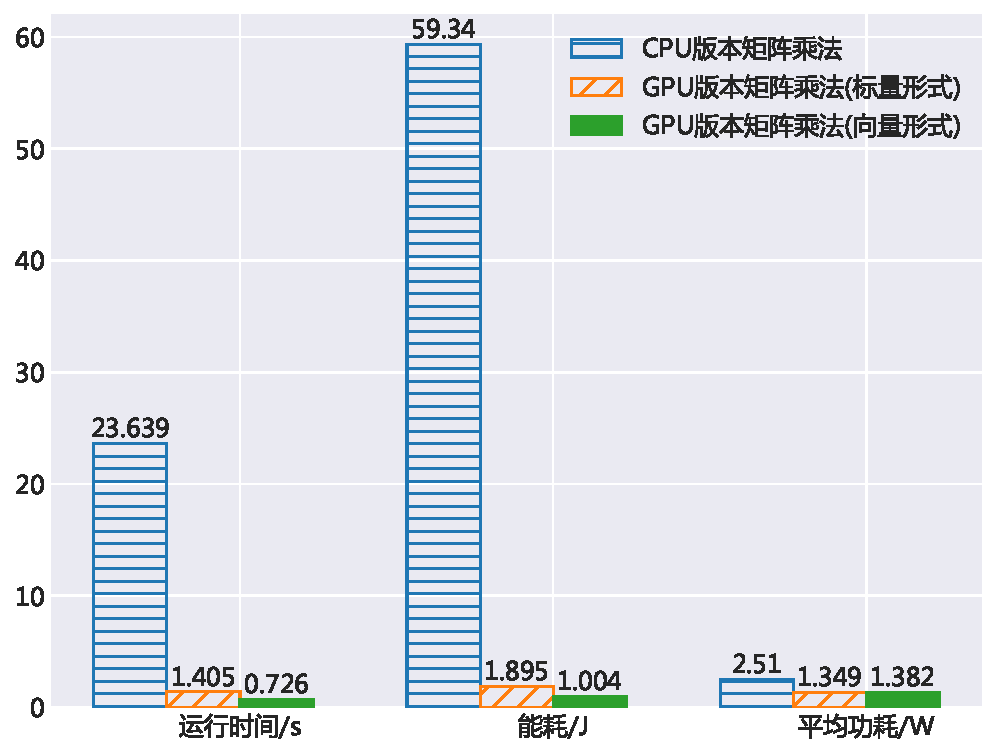
\includegraphics[height=0.4\textwidth]{figures/matmul.pdf}
    \end{center}
    \caption{矩阵乘法不同实现版本的运行时间、能耗和功耗对比}\label{figure:figure9}
\end{figure}

\begin{table}[htbp]
  \centering
  \caption{矩阵乘法不同实现版本的能效对比}
  \label{table:table1}
  \begin{tabular}{cc}
    \toprule
      实现版本 & EDP(Joules*seconds) \\
    \midrule
      CPU版本矩阵乘法 & 1402.763 \\
      GPU版本矩阵乘法(标量形式) & 2.663 \\
      GPU版本矩阵乘法(向量形式) & 0.729 \\
    \bottomrule
  \end{tabular}
\end{table}

由图\ref{figure:figure9}可知,使用手机GPU实现矩阵乘法可以明显提升运算性能并降低运行时能耗和功耗。对于$512\times1024$矩阵与$1024\times512$矩阵的乘积运算,相较于CPU实现版本,GPU的标量实现形式加速比为16.82。另一方面,通过比较GPU版本矩阵乘法的标量实现形式和向量实现形式,可以发现使用OpenCL的\texttt{float4}向量数据类型可以再获得约2倍的性能提升并可进一步降低运行时能耗。由表\ref{table:table1}可知,GPU版本矩阵乘法在能效方面远高于CPU版本矩阵乘法,尤其在使用OpenCL向量数据类型实现时GPU版本的能效提升了近两千倍(EDP的定义见\ref{chapter:edp},其值越小说明能效越高)。

\subsection{卷积层基本算子}

卷积层的基本算子即为卷积操作,这在第二章进行了相关介绍。然而,为了提高卷积操作的执行性能,本章中采用\texttt{img2col}和通用矩阵乘的方式实现卷积操作。

在介绍\texttt{img2col}之前,此处先回顾一下第二章介绍的卷积实现理论细节:卷积核是一个包含权重的小窗口,其在输入图像上按步长滑动,每次滑动会对输入图像上对应的小窗口区域进行操作,即将卷积核中的各个权值与输入图像上对应小窗口中的各个像素值相乘再求和,最后加上偏置得到特征图上的一个输出值。根据上述描述可知,卷积核对输入图的每一次运算与两个向量的内积非常类似。因此,卷积操作完全可以转化为矩阵乘法来实现。为了达到这一目的,需要进行两步操作:(1)使用\texttt{img2col}将输入特征图转换为通过矩阵乘法实现卷积操作时所需的矩阵形式;(2)使用矩阵乘法将权重矩阵与第一步转化而来的矩阵进行相乘以得到卷积输出结果。

\begin{figure}[htb]
    \begin{center}
    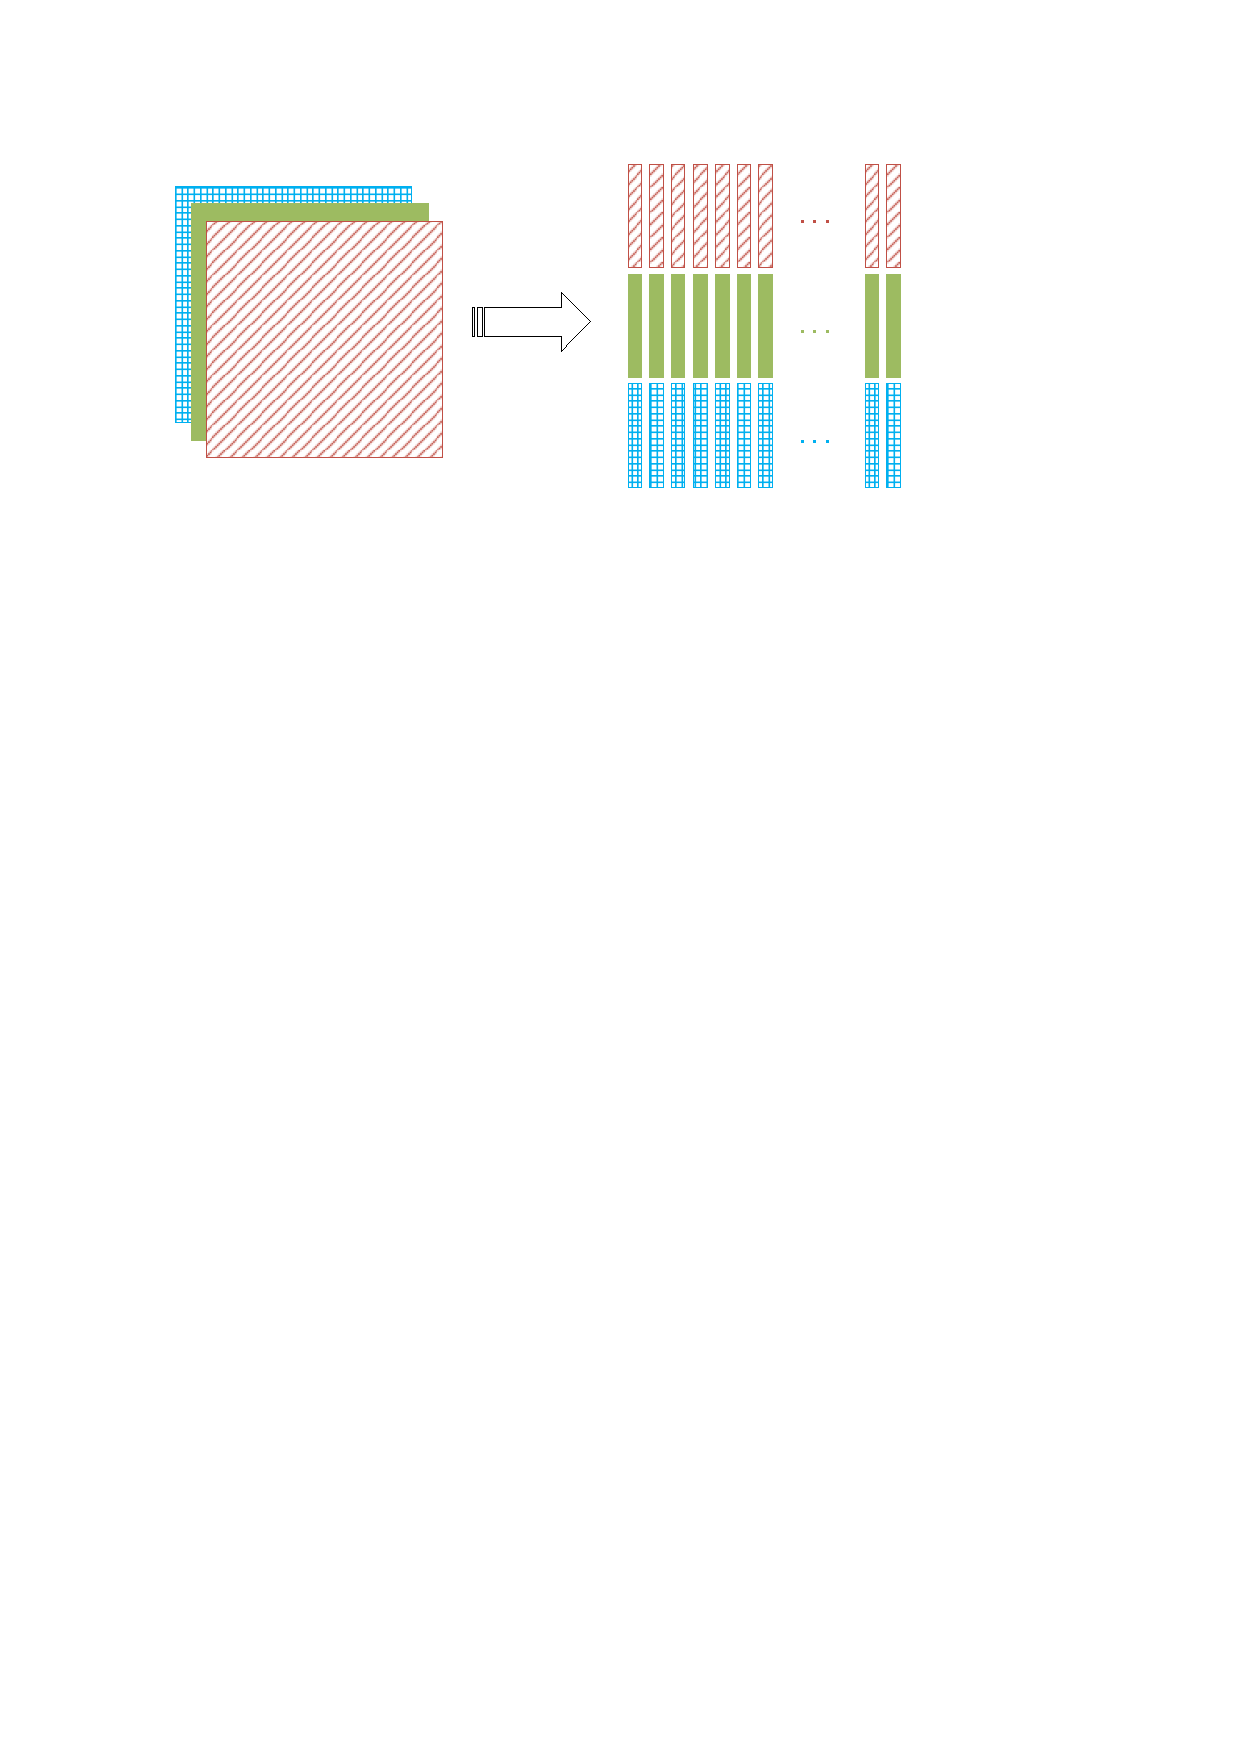
\includegraphics[height=0.3\textwidth]{figures/im2col.pdf}
    \end{center}
    \caption{\texttt{img2col}转换三通道输入特征图示例}\label{figure:figure10}
\end{figure}

图\ref{figure:figure10}给出了一个使用\texttt{img2col}将三通道输入特征图转换为所需输出矩阵的示例,而\texttt{img2col}的执行过程在算法\ref{algo:algorithm4}进行了详细描述。

\begin{algorithm}[htbp]
  \small
  \SetAlgoLined
    \begin{spacing}{0.8}
    \KwData{channels, channel\_size, kernel\_h,kernel\_w, output\_h,output\_w}
    channels,channel\_size分别表示输入通道数和一个通道的数据量\;
    kernel\_h,kernel\_w分别表示卷积核的高度和宽度\;
  output\_h,output\_w分别表示卷积层输出图像的高度和宽度\;
    \For{channel in 0 ... channels-1} {
        \For{kernel\_row in 0 ... kernel\_h-1} {
            \For{kernel\_col in 0 ... kernel\_w-1} {
                计算卷积核中第kernel\_row行在输入图像中的第一个操作区域的行索引\;
                \For{output\_rows in output\_h ... 1} {
                    \If{计算得到的输入图像的行值索引小于零或者大于输入图像的高} {
                        \For{output\_cols in output\_w ... 1} {
                            将该行在输出矩阵上的位置置为0\;
                        }
                    } \Else {
                        计算卷积核中的第kernel\_col列在输入图像中的第一个操作区域的列索引\;
                        \For{output\_col in output\_w ... 1} {
                            \If{输入图像的列值索引大于等于于零或者小于输入图像的宽} {
                                将输入特征图上对应的区域放到输出矩阵上;
                            } \Else {
                                将该行该列在输出矩阵上的位置置为0\;
                            }
                            将输出列坐标移动到下一个卷积窗口\;
                        }
                    }
                    将输出行坐标移动到下一个卷积窗口\;
                }
            }
        }
        将输出矩阵偏移channel\_size以操作下一个输入通道的图像数据\;
    }
    \end{spacing}
  \caption{\texttt{img2col}核心操作伪代码}
  \label{algo:algorithm4}
\end{algorithm}

根据算法\ref{algo:algorithm4}描述的伪代码,本文分别于手机GPU和CPU上实现了\texttt{img2col}操作。为了比较\texttt{img2col}在手机GPU和CPU上的执行性能,本文基于ODROID-XU3平台测量了\texttt{img2col}在处理高度和宽度均为256、通道数为100的输入特征图(步长为1,卷积核大小为$3 \times 3$并且无padding处理)的运行时间、能耗和功耗特征,测量结果如图\ref{figure:figure11}所示。

\begin{figure}[htbp]
    \begin{center}
    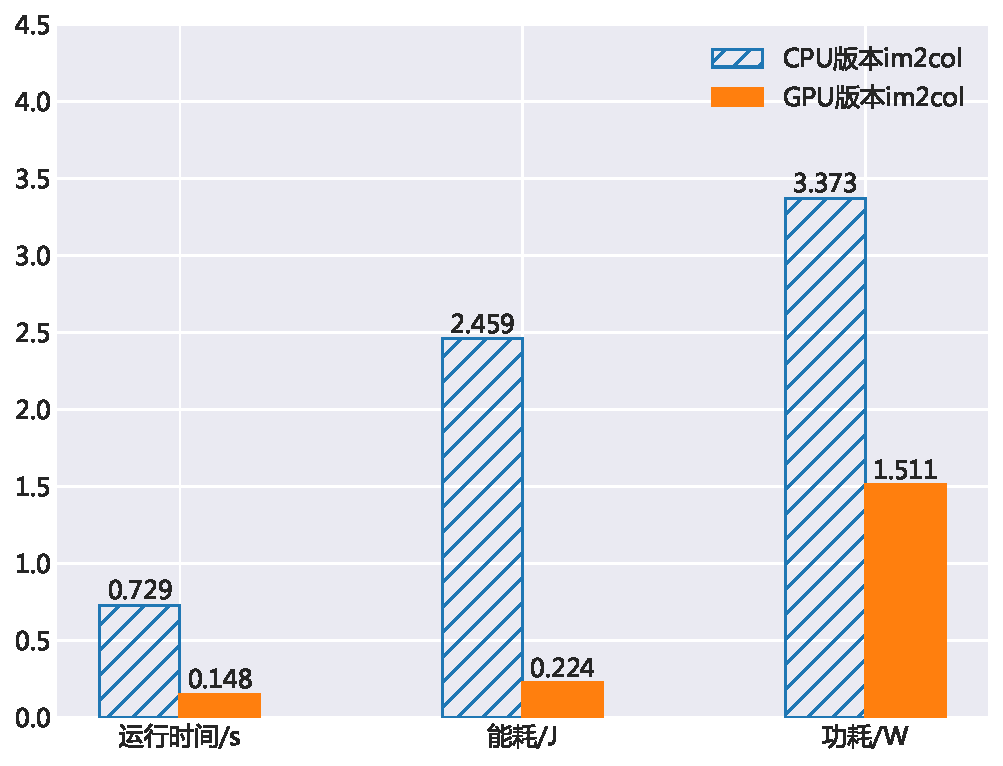
\includegraphics[height=0.4\textwidth]{figures/im2col_energy.pdf}
    \end{center}
    \caption{\texttt{img2col}不同实现版本的运行时间、能耗和功耗对比}\label{figure:figure11}
\end{figure}

由图\ref{figure:figure11}可知,在操作高度和宽度均为256、通道数为100的输入特征图时,相较于CPU版本的\texttt{img2col},GPU版本的\texttt{img2col}可使得执行速度提升5倍左右。与此同时,使用GPU执行\texttt{img2col}操作的能耗仅为使用CPU能耗的1/10,而功耗也降低为使用CPU时的1/2。表\ref{table:table2}显示了GPU版本\texttt{img2col}和CPU版本\texttt{img2col}的EDP值。对比两者的EDP值可知,基于GPU实现的\texttt{img2col}可以将能效提升50倍以上。

\begin{table}[htbp]
  \centering
  \caption{\texttt{img2col}不同实现版本的能效对比}
  \label{table:table2}
  \begin{tabular}{cc}
    \toprule
      实现版本 & EDP(Joules*seconds) \\
    \midrule
      CPU版本im2col & 1.792 \\
      GPU版本im2col & 0.033 \\
    \bottomrule
  \end{tabular}
\end{table}


\subsection{池化层基本算子}

显然,池化层的基本算子即为池化单元。由第\ref{chapter:chapter2-1-2}章节可知,最大池化是目前研究工作中最为常用的池化单元,因此本文主要实现了最大池化操作。根据第\ref{chapter:chapter2-1-2}章节中对最大池化操作的自然语言描述,可形成如算法\ref{algo:algorithm5}所示的最大池化操作伪代码。同样地,本文于手机GPU和CPU上分别实现了算法\ref{algo:algorithm5}所描述的伪代码。

\begin{algorithm}[htbp]
  \small
  \SetAlgoLined
    \begin{spacing}{0.8}
    \KwData{channels, pooled\_h, pooled\_w}
    channels表示输入通道数\;
    pooled\_h和pooled\_w分别表示池化输出矩阵的高度和宽度\;
    \For{c in 0 ... channels-1} {
        \For{ph 0 ... pooled\_h-1} {
            \For{pw in 0 ... pooled\_w-1} {
                计算本次池化窗口的行操作起始位置hstart和终止位置hend\;
                计算本次池化窗口的列操作起始位置wstart和终止位置wend\;
                确保本次行列操作起始位置hstart和wstart均为非负值\;
                计算本次池化操作输出矩阵的对应下标pool\_index\;
                将本次池化窗口左上角第一个值赋给输出矩阵下标为pool\_index的项\;

                \For{h in hstart ... hend-1} {
                    \For{w in wstart ... wend-1} {
                      利用上面两重循环遍历本次池化窗口中每一个值value\;
                        将value与输出矩阵下标为pool\_index的项做比较\;
                      将两者较大值重新赋值给输出矩阵下标为pool\_index的项\;
                    }
                }
            }
        }
        将输入特征图偏与输出矩阵均偏移到下一个通道\;
    }
    \end{spacing}
  \caption{最大池化核心操作伪代码}
  \label{algo:algorithm5}
\end{algorithm}

%\begin{figure}[htbp]
%\begin{minipage}[b]{.6\linewidth}
%    \begin{center}
%    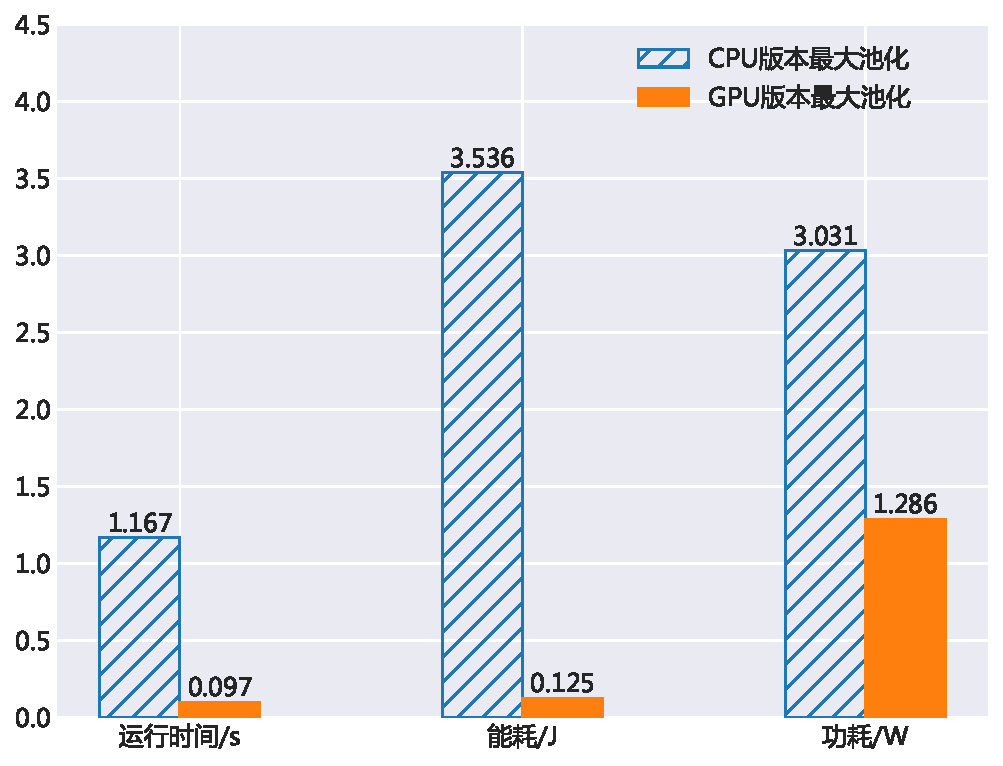
\includegraphics[height=0.65\textwidth]{figures/pool_energy.pdf}
%    \end{center}
%    \captionsetup{font={small}}
%    \caption{最大池化不同实现版本的运行时间、\\能耗和功耗对比}\label{figure:figure12}
%\end{minipage}
%\begin{minipage}[b]{.4\linewidth}
%\centering
%\resizebox{1.0\textwidth}{!}{
%\begin{tabular}{cc}
%    \toprule
%      实现版本 & EDP(Joules*seconds) \\
%    \midrule
%      CPU版本最大池化 & 4.125 \\
%      GPU版本最大池化 & 0.012 \\
%    \bottomrule
%\end{tabular}
%}
%\captionsetup{font={small}}
%\captionof{table}{最大池化不同实现版本的\\能效对比}\label{table:table3}
%\end{minipage}
%\end{figure}

对于一张高度和宽度均为256、通道数为100的输入特征图,本文测量了其在ODROID-XU3平台上进行最大池化操作所需的运行时间、能耗和功耗。实验中,池化操作的步长取为1、池化核大小取为$3 \times 3$,并且不进行padding处理。测量结果如图\ref{figure:figure12}所示。

\begin{figure}[htb]
    \begin{center}
    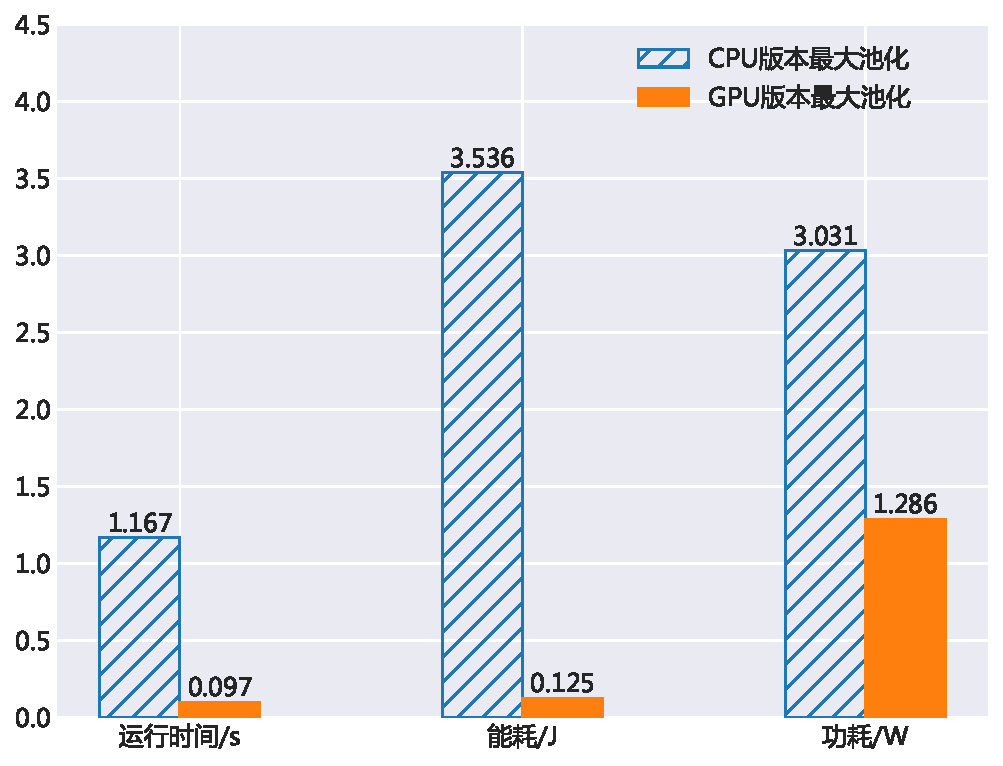
\includegraphics[height=0.4\textwidth]{figures/pool_energy.pdf}
    \end{center}
    \caption{最大池化不同实现版本的运行时间、能耗和功耗对比}\label{figure:figure12}
\end{figure}

由图\ref{figure:figure12}可知,使用GPU进行最大池化操作不仅可以将运算速度提升12倍还可以把能耗降为使用CPU时的1/28。最大池化在CPU和GPU上执行的功耗特征与\texttt{img2col}类似,即GPU版本最大池化功耗约为CPU版本最大池化功耗的一半。表\ref{table:table3}从能效的角度分析了最大池化在不同计算设备上的表现,即GPU版本最大池化的能效要高出CPU版本约300余倍。

\begin{table}[htbp]
  \centering
  \caption{最大池化不同实现版本的能效对比}
  \label{table:table3}
  \begin{tabular}{cc}
    \toprule
      实现版本 & EDP(Joules*seconds) \\
    \midrule
      CPU版本最大池化 & 4.125 \\
      GPU版本最大池化 & 0.012 \\
    \bottomrule
  \end{tabular}
\end{table}

\subsection{激活层基本算子}

正如第\ref{chapter:chapter2-1-4}章节所述,激活层主要使用非线性激活函数对输入数据进行处理,故而激活层的基本算子即为所使用的激活函数。在具体实现中,可选的激活函数主要有Relu函数、Sigmod函数以及双曲正切函数等。选定激活函数\texttt{activation\_fun()},激活层基本算子的实现伪代码可表示如下:

\begin{algorithm}[htbp]
  \small
  \SetAlgoLined
  \KwData{data, length}
  \For{i in 0 ... length-1}{
        data[i]=activation\_fun(data[i])\;
  }
  \caption{激活层基本算子实现伪代码}
  \label{algo:algorithm6}
\end{algorithm}

\begin{figure}[htb]
    \begin{center}
    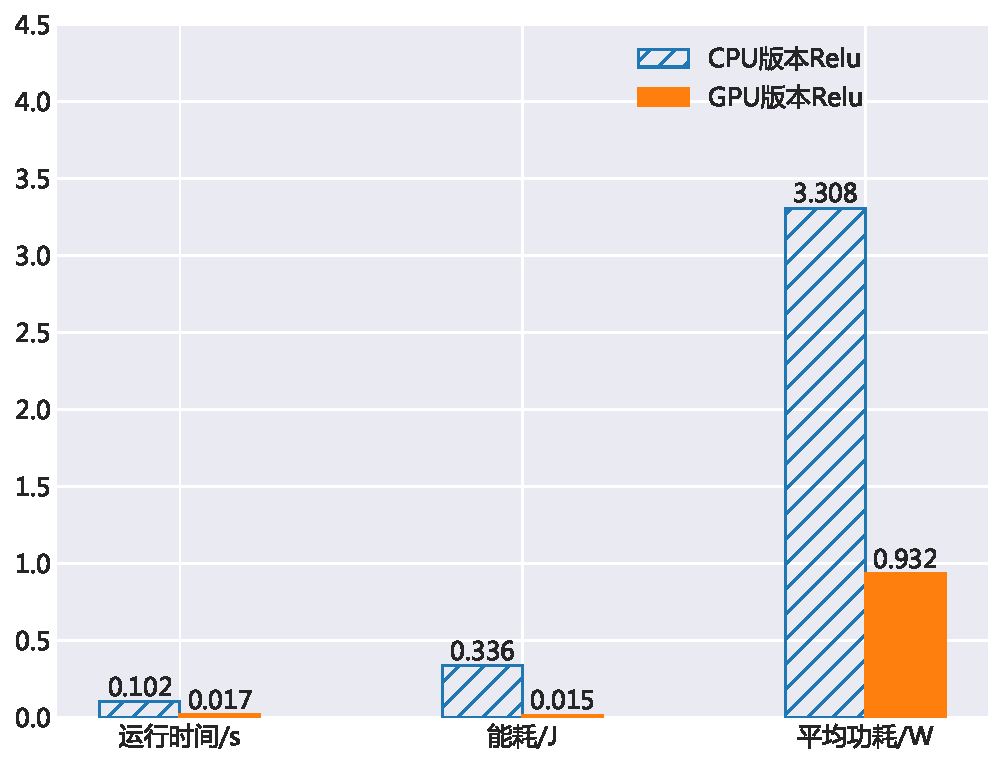
\includegraphics[height=0.4\textwidth]{figures/relu_energy.pdf}
    \end{center}
    \caption{Relu激活算子不同实现版本的运行时间、能耗和功耗对比}\label{figure:figure13}
\end{figure}

根据算法\ref{algo:algorithm6}所描述的实现逻辑,本文分别实现了基于手机GPU和CPU的激活操作。图\ref{figure:figure13}显示了Relu激活算子分别于手机GPU和CPU上处理$100 \times 256 \times 256 $个输入数据时的运行时间、能耗和功耗。可以看出,在输入数据量为$100 \times 256 \times 256 $时,GPU版本Relu激活算子的执行速度可比CPU版本的快6倍,并同时可降低22倍的能耗和3.5倍的功耗。表\ref{table:table4}给出Relu激活算子分别在CPU和GPU上运行时的能效。其中,CPU版本Relu激活算子的EDP为0.034,而GPU版本Relu激活算子的EDP仅为0.0003。根据EDP值越小能效越高的度量标准可知,在输入数据量为$100 \times 256 \times 256 $时,Relu激活算子在GPU上的运行时能效是其在CPU上运行时能效的100多倍。

\begin{table}[htbp]
  \centering
  \caption{Relu激活算子不同实现版本的能效对比}
  \label{table:table4}
  \begin{tabular}{cc}
    \toprule
      实现版本 & EDP(Joules*seconds) \\
    \midrule
      CPU版本Relu激活算子 & 0.034 \\
      GPU版本Relu激活算子 & 0.0003 \\
    \bottomrule
  \end{tabular}
\end{table}

%\begin{figure}[htbp]
%\begin{minipage}[b]{.6\linewidth}
%    \begin{center}
%    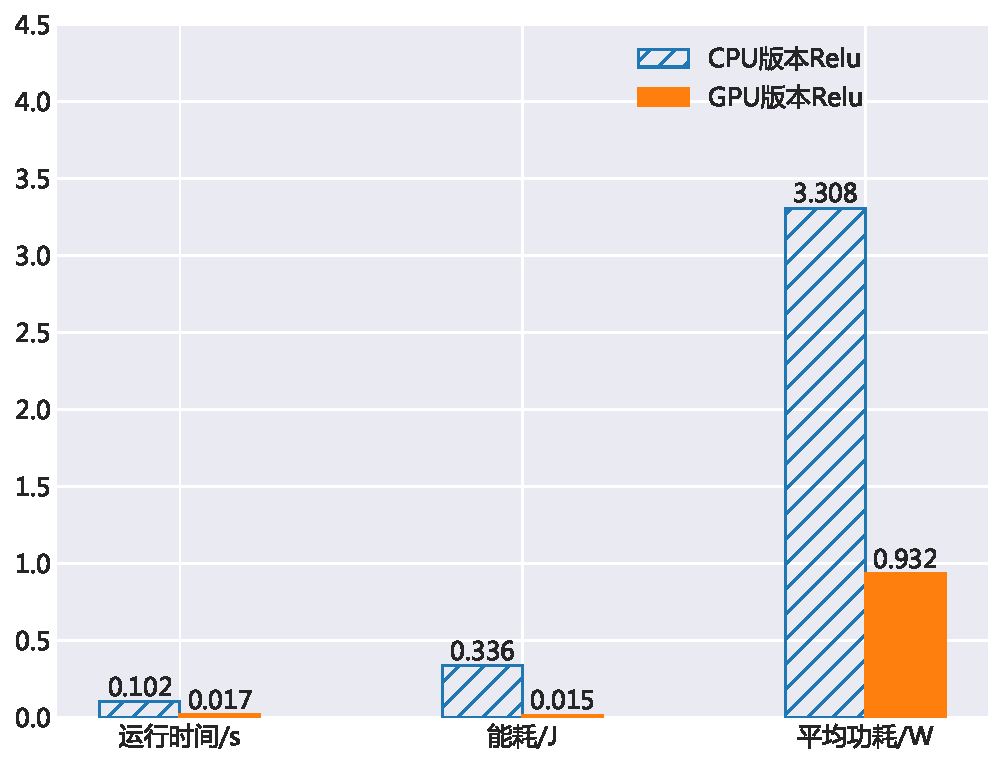
\includegraphics[height=0.65\textwidth]{figures/relu_energy.pdf}
%    \end{center}
%    \captionsetup{font={small}}
%    \caption{Relu激活算子不同实现版本的运行时间、\\ 能耗和功耗对比}\label{figure:figure13}
%\end{minipage}
%\begin{minipage}[b]{.4\linewidth}
%\centering
%\resizebox{1.0\textwidth}{!}{
%\begin{tabular}{cc}
%    \toprule
%      实现版本 & EDP(Joules*seconds) \\
%    \midrule
%      CPU版本Relu激活算子 & 0.034 \\
%      GPU版本Relu激活算子 & 0.0003 \\
%    \bottomrule
%\end{tabular}
%}
%\captionsetup{font={small}}
%\captionof{table}{Relu激活算子不同实现版本的能效对比}\label{table:table4}
%\end{minipage}
%\end{figure}

\section{基于手机GPU加速的CNN前向推断}

第\ref{chapter:chapter3-1}章节对卷积神经网络前向推断过程中所涉及的基本算子进行了分解与实现,而本章节即利用这些基本算子分别实现了基于手机GPU和CPU的CNN前向推断过程所需层结构,包括卷积层、池化层、全连接层和激活层等。利用所实现的各种层结构,本章节于手机端重构了LeNet-5和AlexNet模型,并分析比较了两个模型在手机GPU和CPU上运行时的能效特征。

\subsection{预训练CNN模型权重参数解析}
\label{chapter:chapter321}

\begin{figure}[htbp]
    \begin{center}
    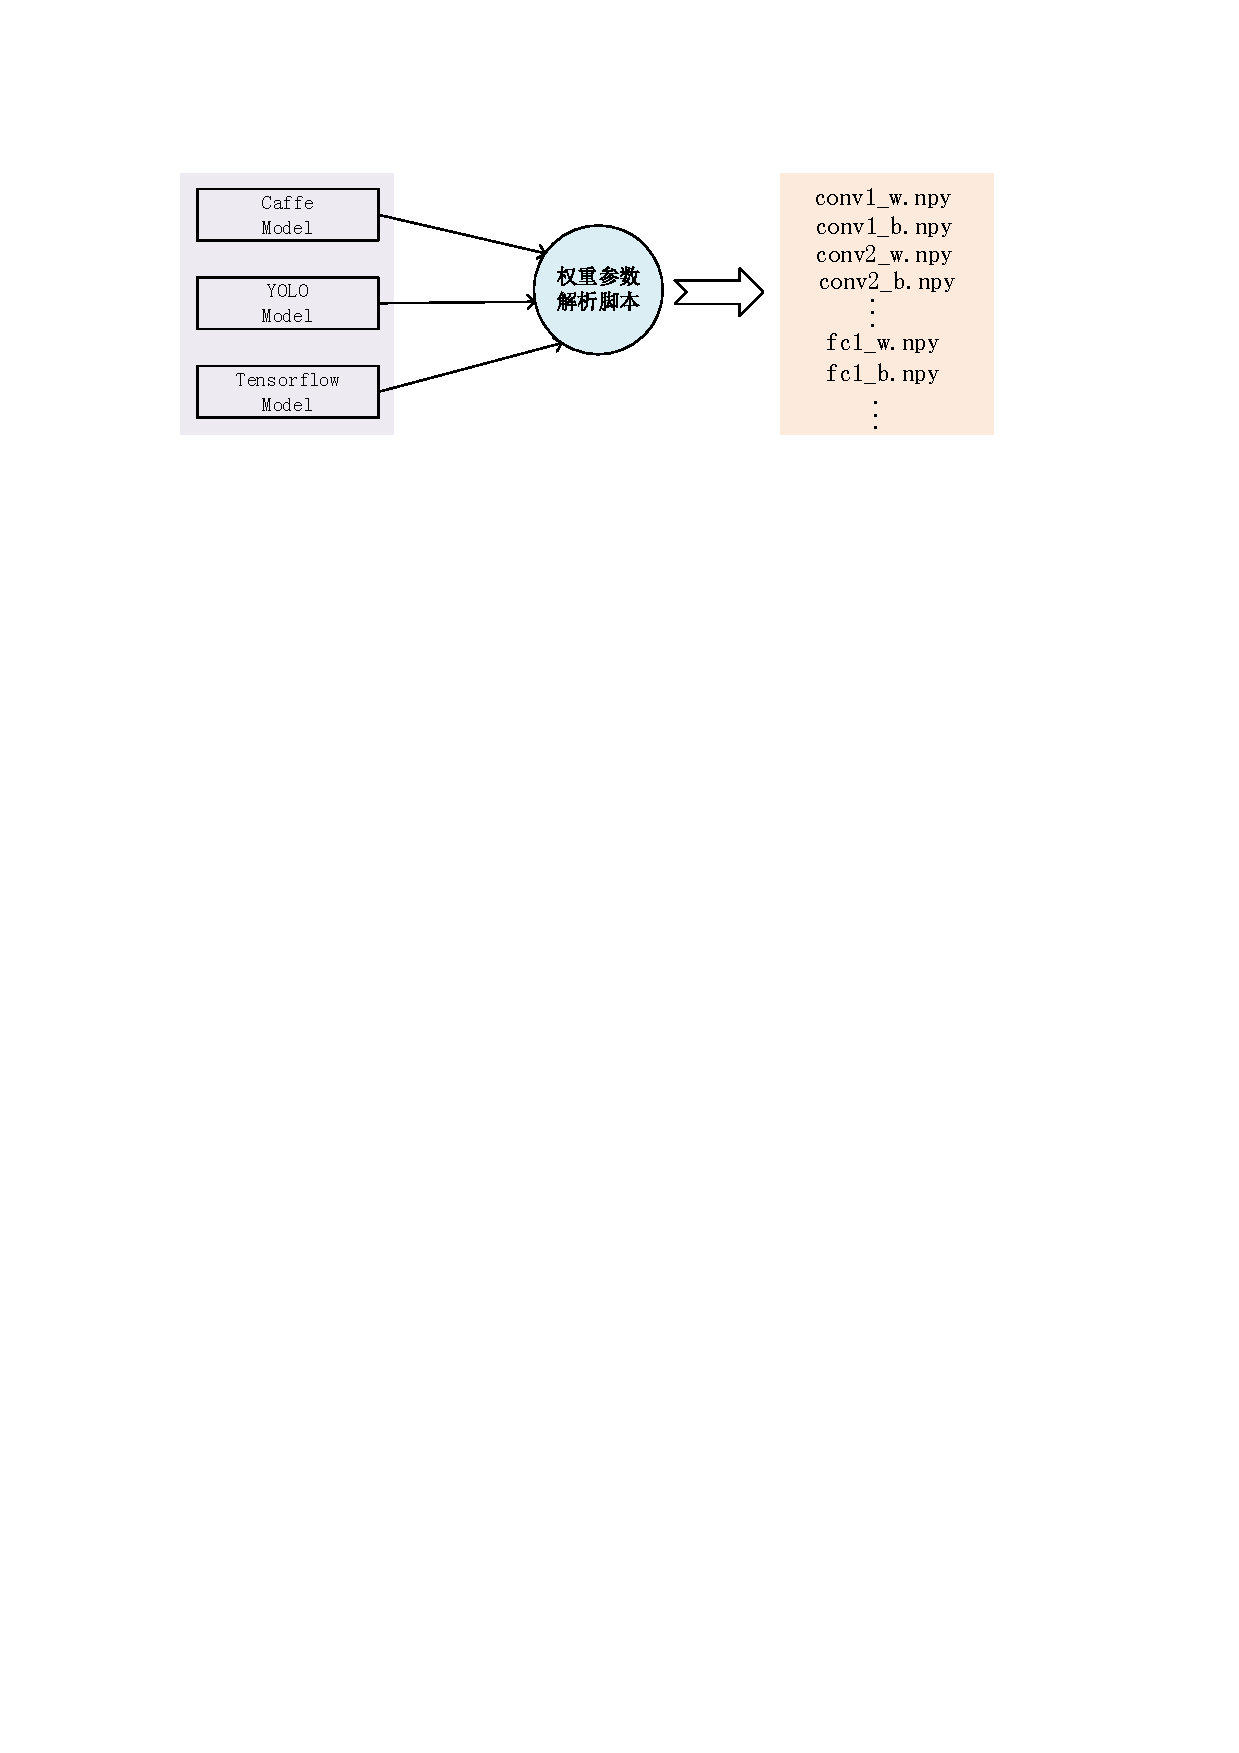
\includegraphics{figures/weight.pdf}
    \end{center}
    \caption{CNN模型权重参数解析流程概览}\label{figure:figure14}
\end{figure}

解析预训练CNN模型权重参数是在手机端重构卷积神经网络前向推断过程的首要条件,本文针对Caffe、YOLO和Tensorflow等深度学习框架所训练的CNN模型给出了权重解析的python脚本。该脚本可以提取预训练CNN模型的每层权重参数(权值矩阵和偏置矩阵等),并将这些权重参数分层保存为二进制npy文件格式,整个流程如图\ref{figure:figure14}所示。

\subsection{LeNet-5模型于手机端的重构}

\begin{figure}[htbp]
    \centering
    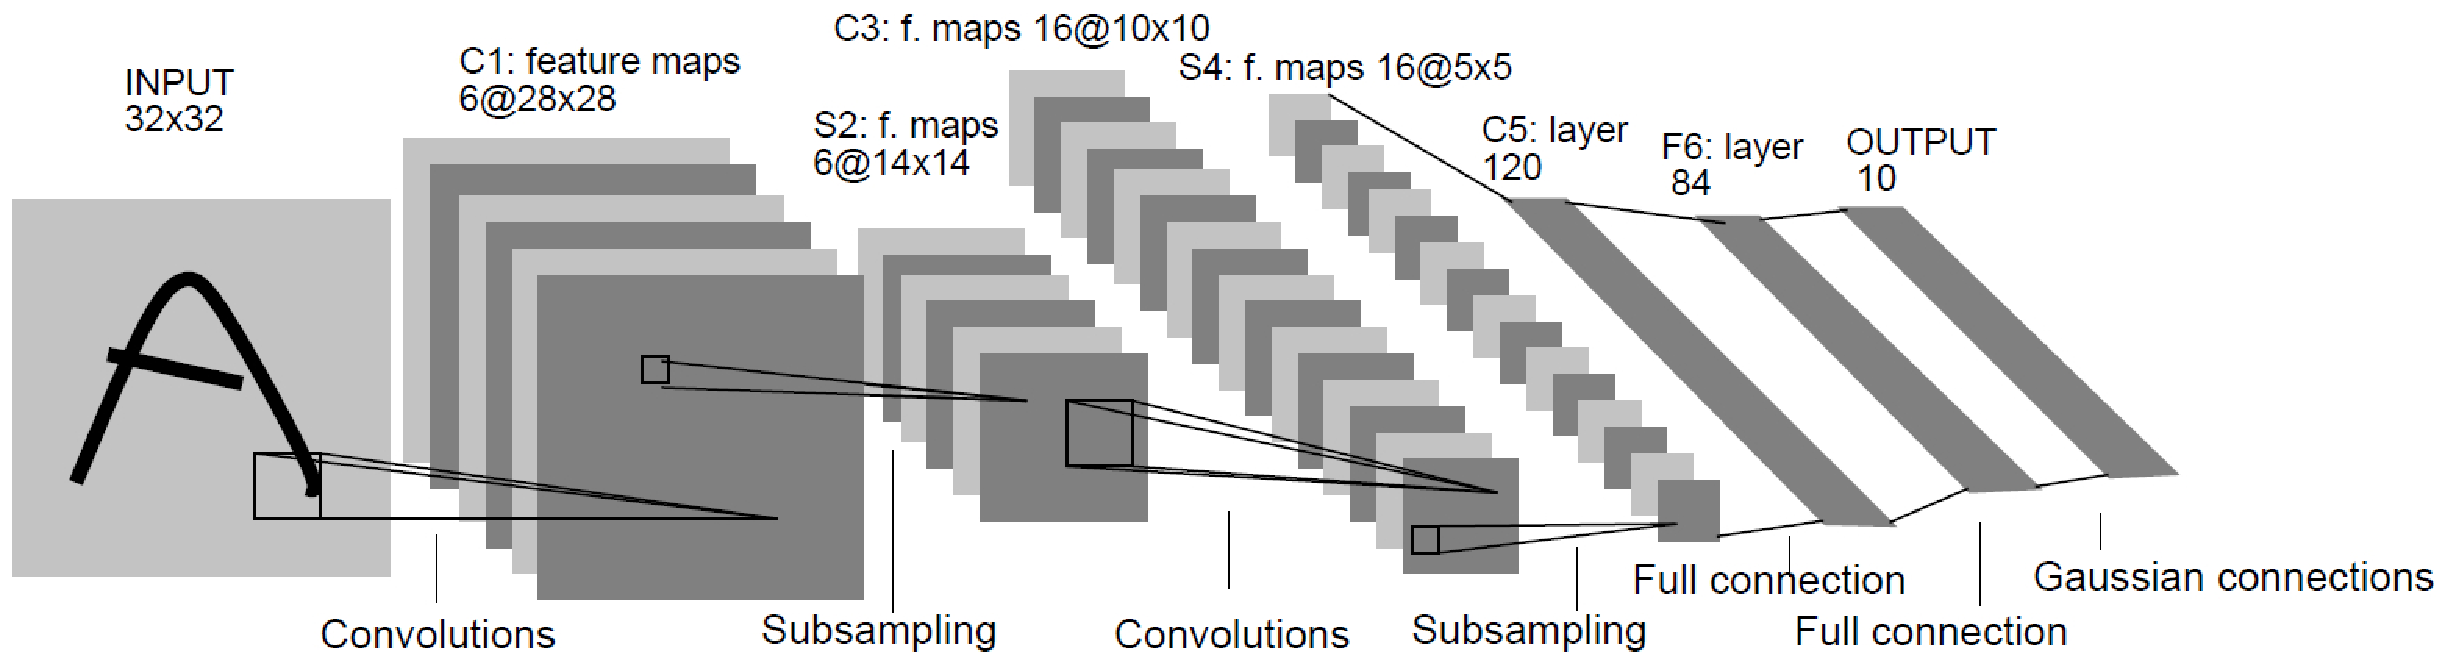
\includegraphics[width=1.0\textwidth]{figures/lenet.pdf}
    \caption{LeNet-5模型结构示意图 \cite{lecun1998gradient}}\label{figure:figure15}
\end{figure}

LeNet-5是由卷积神经网络之父Yan LeCun提出的,其主要用来进行手写字符的识别与分类。原始的LeNet-5模型主要由2个卷积层、2个池化层、1个全连接层以及1个高斯连接层组成,如图\ref{figure:figure15}所示。本文所采用的LeNet-5模型将最后一层高斯连接层替换为了全连接层,且在MNIST数据集\cite{lecun.com}上的预测精度可达99.1\%。表\ref{table:table5}描述了本文所采用的LeNet-5模型结构中卷积层和全连接层的参数信息。
\vspace{-1.5em}
\begin{table}[htbp]
  \centering
  \caption{LeNet-5模型结构中的卷积层和全连接层}
  \label{table:table5}
\resizebox{1.0\textwidth}{!}{
  \begin{tabular}{ccc}
    \toprule
      名称 & 类型 & 描述\\
    \midrule
      conv1 & 卷积层 & 输入:$1\times28\times28$,卷积核:$20\times1\times5\times5$,步长:1,padding:0,输出:$20\times24\times24$ \\
      conv2 & 卷积层 & 输入:$20\times12\times12$,卷积核:$50\times20\times5\times5$,步长:1,padding:0,输出:$50\times8\times8$\\
      ip1 & 全连接层 & 输入:800, 输出:500 \\
      ip2 & 全连接层 & 输入:500, 输出:10 \\
    \bottomrule
  \end{tabular}
}
\end{table}
\vspace{-0.5em}

利用第\ref{chapter:chapter321}章节的权重解析脚本,可获取到LeNet-5模型各层的权重参数矩阵。基于这些权值矩阵,本文分别于手机GPU和CPU上重构了LeNet-5模型,图\ref{figure:figure16}显示了LeNet-5模型在ODROID-XU3平台上进行单张图片前向推断所需的运行时间、能耗和功耗。

\begin{figure}[htbp]
    \centering
    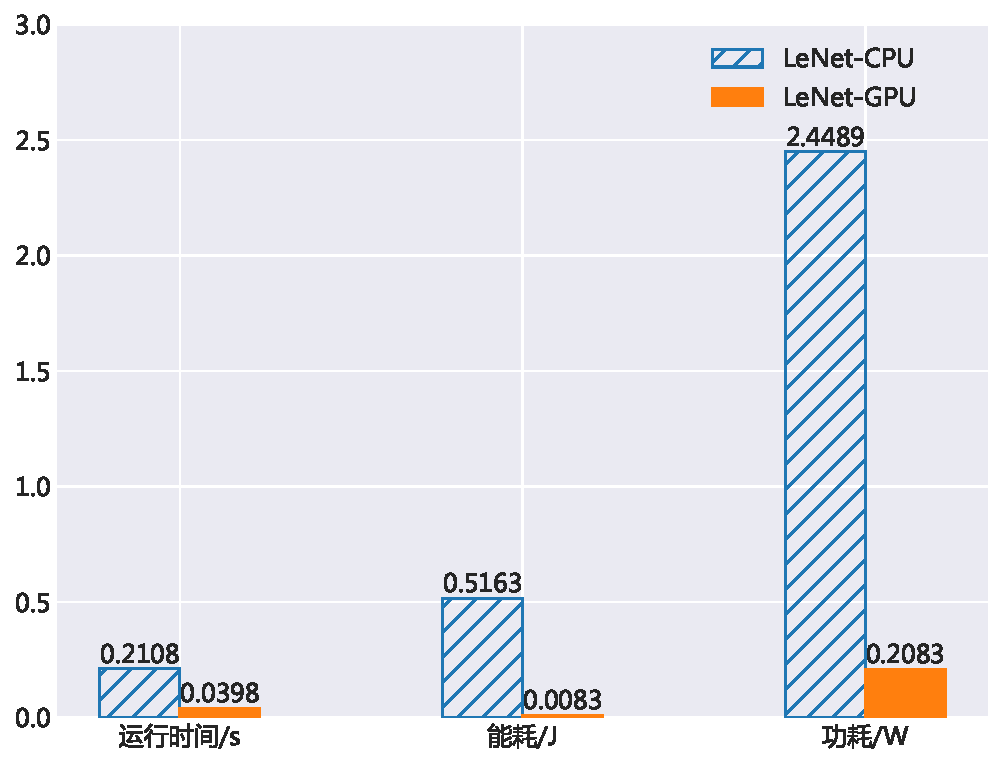
\includegraphics[height=0.4\textwidth]{figures/lenet_energy.pdf}
    \caption{ODROID-XU3平台上LeNet-5单张图片推断运行时间、能耗和功耗对比}\label{figure:figure16}
\end{figure}

由图\ref{figure:figure16}可知,LeNet-5模型在手机GPU上进行前向推断的执行速度是在手机CPU上的11倍以上,并且可以节省120多倍的能耗。根据表\ref{table:table6}显示的LeNet-5模型分别于手机GPU和CPU上运行时EDP值可知,使用手机GPU进行LeNet-5的前向推断可以将能效提升1350倍以上。

\begin{table}[htbp]
  \centering
  \caption{LeNet-5分别于手机GPU和CPU上运行时能效对比}
  \label{table:table6}
  \begin{tabular}{cc}
    \toprule
      运行处理器 & EDP(Joules*seconds) \\
    \midrule
      CPU & 0.0982 \\
      GPU & 0.00007 \\
    \bottomrule
  \end{tabular}
\end{table}

对比图\ref{figure:figure16}和图\ref{figure:figure11}中手机GPU功耗值,可以发现LeNet-5模型于手机GPU进行前向推断时并未充分利用GPU的计算性能。这是因为使用手机GPU进行\texttt{im2col}运算时其功耗为1.511瓦,而使用手机GPU进行LeNet-5前向推断时其功耗仅为0.2413瓦。这可能是因为LeNet-5模型太小,未能充分发挥GPU的并行计算能力。为了验证这一猜想,本文进一步于手机端重构了AlexNet模型。

\subsection{AlexNet模型于手机端的重构}

\begin{figure}[htbp]
    \centering
    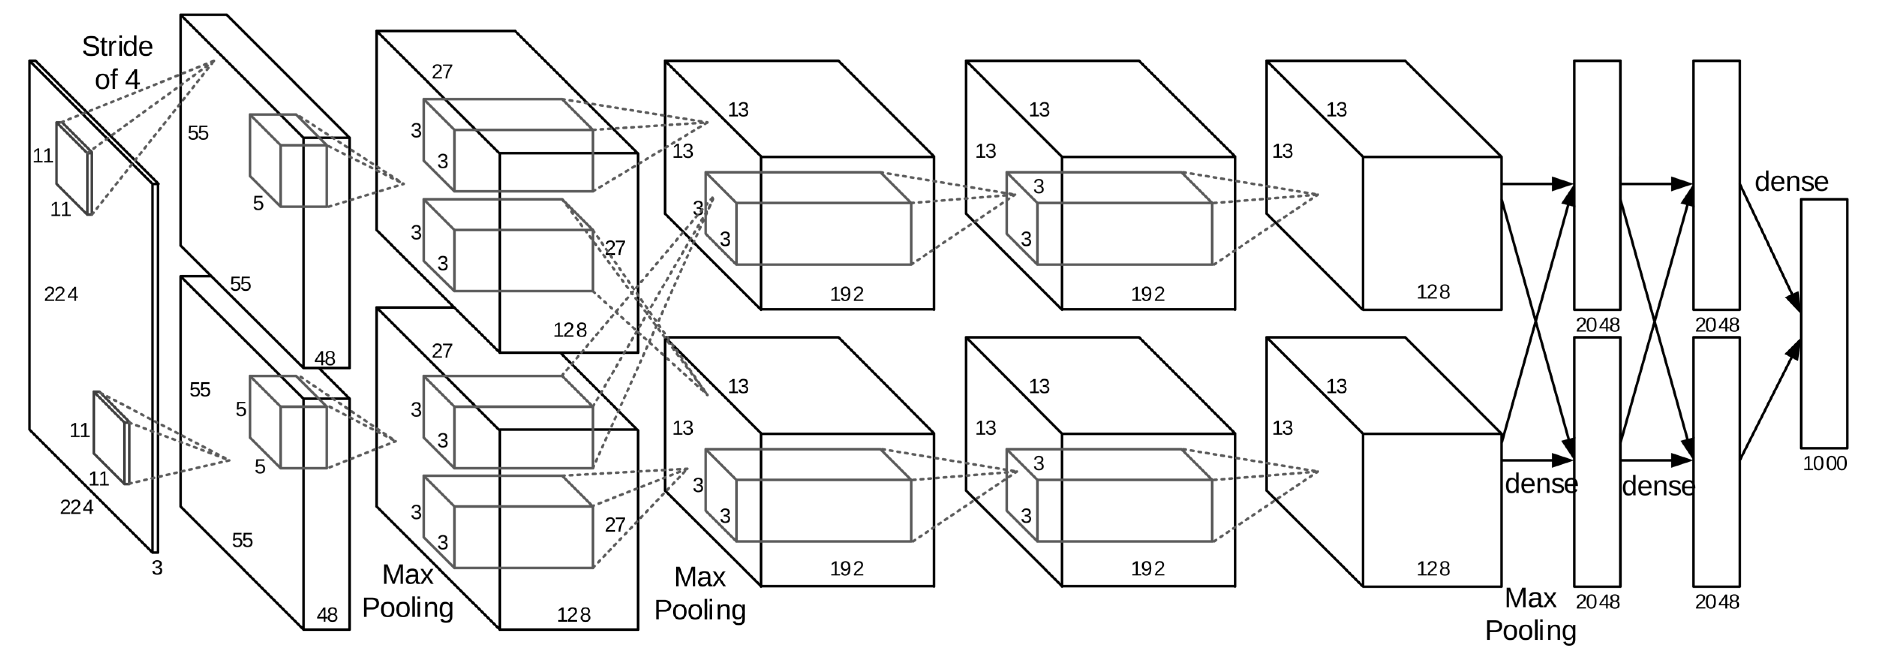
\includegraphics[width=1.0\textwidth]{figures/alexnet.pdf}
    \caption{AlexNet模型结构示意图 \cite{krizhevsky2012imagenet}}\label{figure:figure17}
\end{figure}

AlexNet模型在2012年ImageNet大赛上一举夺冠开启了深度学习的新时代,它也为后续的CNN模型研究奠定了基础,其模型结构如图\ref{figure:figure17}所示。AlexNet模型主要由5个卷积层、3个池化层和3个全连接层组成。其中,AlexNet模型的所有权重均包含在卷积层和全连接层,它们的参数信息见表\ref{table:table7}。

\begin{table}[htbp]
  \centering
  \caption{AlexNet模型结构中的卷积层和全连接层}
  \label{table:table7}
\resizebox{1.0\textwidth}{!}{
  \begin{tabular}{ccc}
    \toprule
      名称 & 类型 & 描述\\
    \midrule
      conv1 & 卷积层 & 输入:$3\times227\times227$,卷积核:$96\times3\times11\times11$,步长:4,padding:0,输出:$96\times55\times55$ \\
      conv2 & 卷积层 & 输入:$96\times27\times27$,卷积核:$256\times96\times5\times5$,步长:1,padding:2,输出:$256\times27\times27$\\
      conv3 & 卷积层 & 输入:$256\times13\times13$,卷积核:$384\times256\times3\times3$,步长:1,padding:1,输出:$384\times13\times13$ \\
      conv4 & 卷积层 & 输入:$384\times13\times13$,卷积核:$384\times384\times3\times3$,步长:1,padding:1,输出:$384\times13\times13$\\
      conv5 & 卷积层 & 输入:$384\times13\times13$,卷积核:$256\times384\times3\times3$,步长:1,padding:1,输出:$256\times13\times13$\\
      fc6 & 全连接层 & 输入:9216, 输出:4096 \\
      fc7 & 全连接层 & 输入:4096, 输出:4096 \\
      fc8 & 全连接层 & 输入:4096, 输出:1000 \\
    \bottomrule
  \end{tabular}
}
\end{table}

图\ref{figure:figure18}显示了AlexNet模型分别于ODROID-XU3平台CPU和GPU上进行单张图片推断的运行时间、能耗和功耗对比。与图\ref{figure:figure16}中LeNet-5模型的推断运行相比,AlexNet模型于手机GPU上执行前向推断相较于手机CPU而言加速比可达15。从功耗角度分析可知,AlexNet模型于手机GPU上执行前向推断时手机GPU的功耗(1.31瓦)接近其峰值,这也说明了使用手机GPU加速AlexNet这种较大的CNN模型效果更加明显。虽然AlexNet模型于手机GPU上执行前向推断时的功耗比LeNet-5模型使用GPU执行时的功耗增加了1瓦,但是其仍然只是使用CPU执行AlexNet模型时的一半,也因此其能耗只达到了使用CPU执行AlexNet模型时的1/30。由表\ref{table:table8}显示的EDP值可得使用GPU与CPU分别执行AlexNet模型的能效加速比为472,这充分显示了手机GPU在进行卷积神经网络计算时的优势。

\begin{figure}[htbp]
\begin{minipage}[b]{.6\linewidth}
    \begin{center}
    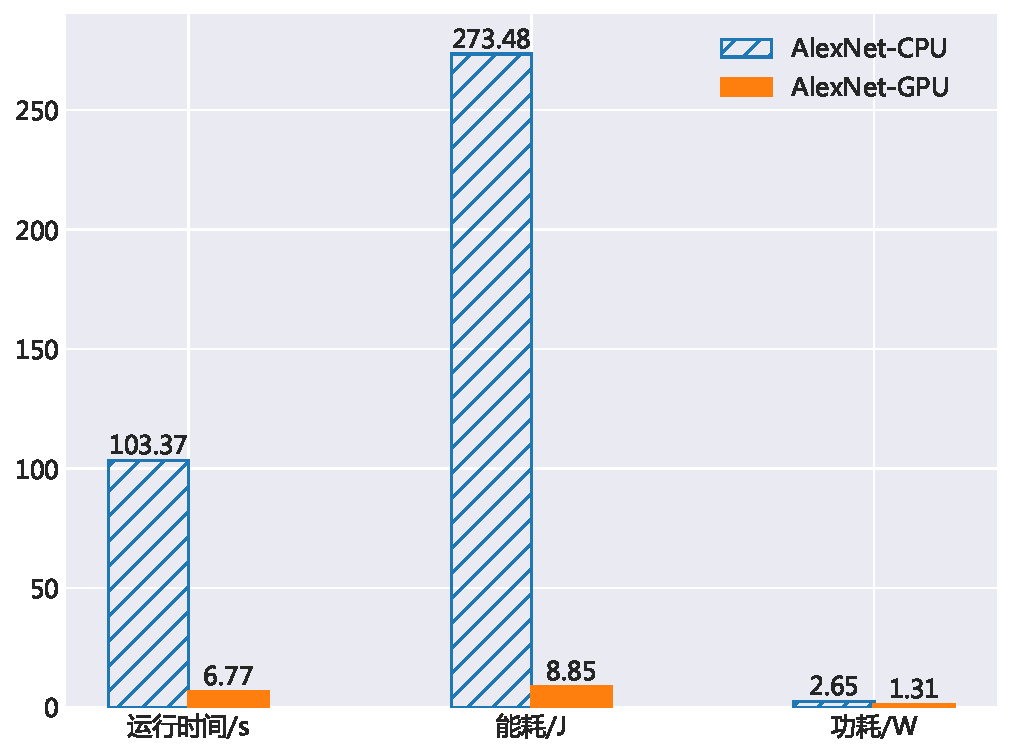
\includegraphics[height=0.65\textwidth]{figures/alexnet_energy.pdf}
    \end{center}
    \captionsetup{font={small}}
    \caption{ODROID-XU3平台上AlexNet单张图片 \\ 推断运行时间、能耗和功耗对比}\label{figure:figure18}
\end{minipage}
\begin{minipage}[b]{.4\linewidth}
\centering
\resizebox{1.0\textwidth}{!}{
\begin{tabular}{cc}
    \toprule
      运行处理器 & EDP(Joules*seconds) \\
    \midrule
      CPU & 28268.24 \\
      GPU & 59.84 \\
    \bottomrule
\end{tabular}
}
\captionsetup{font={small}}
\captionof{table}{AlexNet分别于手机GPU和CPU上运行时能效对比}\label{table:table8}
\end{minipage}
\end{figure}

%\begin{figure}[htbp]
%    \centering
%    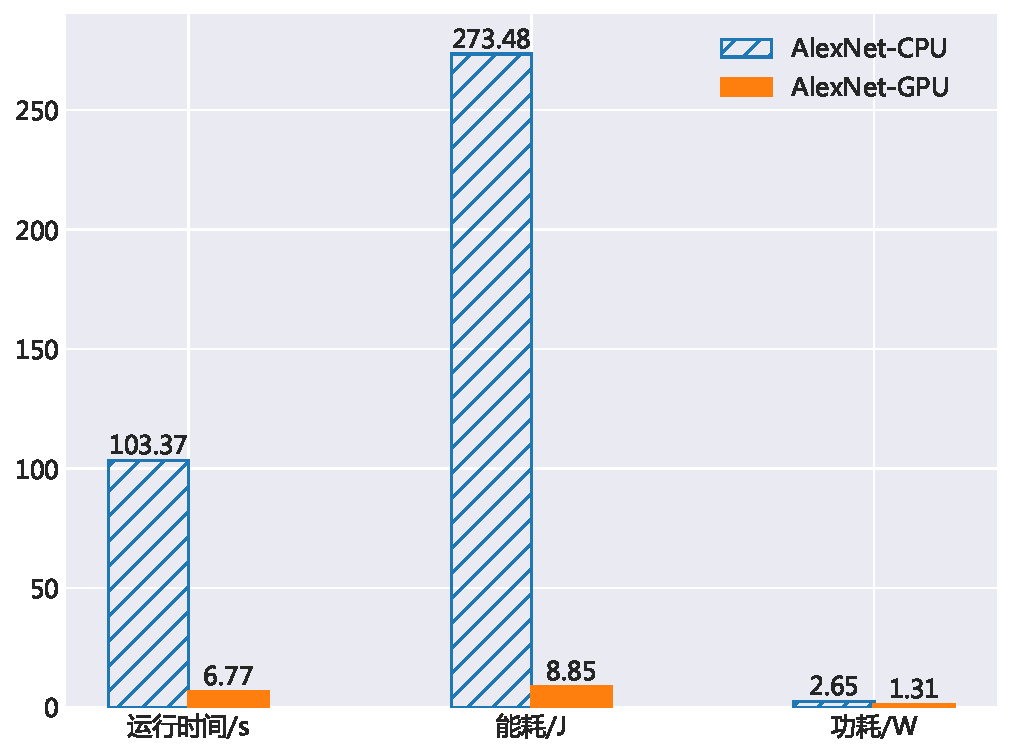
\includegraphics[height=0.45\textwidth]{figures/alexnet_energy.pdf}
%    \caption{ODROID-XU3平台上AlexNet单张图片推断运行时间、能耗和功耗对比}\label{figure:figure18}
%\end{figure}
%
%\begin{table}[htbp]
%  \centering
%  \caption{AlexNet分别于手机GPU和CPU上运行时能效对比}
%  \label{table:table8}
%  \begin{tabular}{cc}
%    \toprule
%      运行处理器 & EDP(Joules*seconds) \\
%    \midrule
%      CPU & 28268.24 \\
%      GPU & 59.84 \\
%    \bottomrule
%  \end{tabular}
%\end{table}

为了验证本文所开发的CNN运行时库的可移植性与兼容性,本文在Open-Q™ 820开发套件上也重构了AlexNet模型。图\ref{figure:figure19}显示了AlexNet模型分别于ODROID-XU3平台和Open-Q™ 820开发套件上进行单张图片推断的CPU运行时间和GPU运行时间。对比分析两个平台上使用CPU进行AlexNet前向推断的运行时间可知,骁龙820的CPU相较于三星Exynos5422的CPU在计算性能上提升了4倍多。对于使用GPU进行CNN前向推断,骁龙820的处理性能更是提升了近7倍,这使得于手机端完成一次完整的AlexNet前向推断仅需要580毫秒。可以看出,手机SoC芯片中的CPU和GPU处理性能都在日趋强大,这为深度学习模型(如卷积神经网络)于手机本地完成离线推断奠定了基础。

\begin{figure}[htbp]
    \centering
    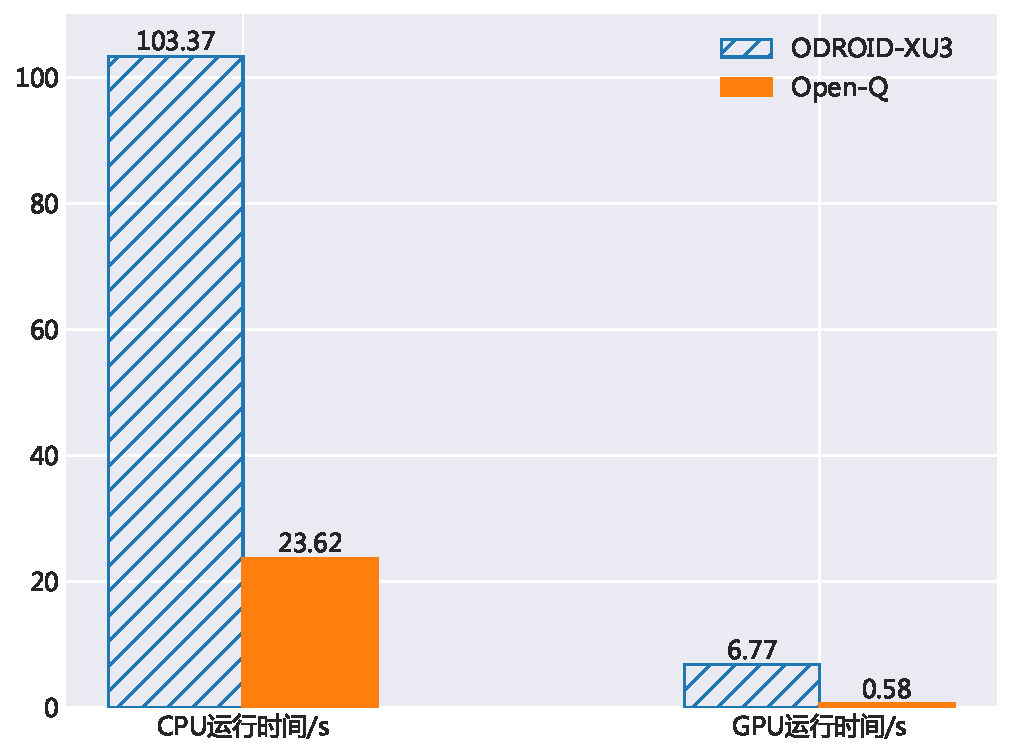
\includegraphics[height=0.4\textwidth]{figures/open_q.pdf}
    \caption{不同平台上AlexNet单张图片推断运行时间对比}\label{figure:figure19}
\end{figure}

\section{基于“剪枝-重训”的层压缩优化}

神经网络是一种典型的过参数化模型,其通常包含着大量的冗余参数(如AlexNet的模型大小约为250M),这会导致计算和内存占用两方面的浪费。然而,手机相较于桌面电脑而言,其往往配备着较低容量的内存,如华为Mate 9 Pro和三星 Galaxy S8的内存大小均为4G。另外需要注意的是,卷积神经网络模型中全连接层参数占了整个网络参数的绝大部分,如AlexNet模型中全连接层参数占整个网络参数的90\%以上。因此,为了降低CNN模型在手机端进行前向推断时的内存占用开销,本文采用“剪枝-重训”方法对CNN模型的全连接层参数进行压缩。

“剪枝”的主体思想就是将不重要的冗余权重连接删除,只保留网络模型中最重要的连接部分。本文参考《Learning both weights and connections for efficient neural network》\cite{han2015learning}一文中的通用剪枝思想将权值的绝对值大小低于某一阈值的连接视为不重要的冗余连接。“重训”即剪枝后重训训练,这主要是为了保证剪枝后网络模型的精确度不损失。很明显,如果直接删除网络模型中的部分连接而不做重新训练处理,那么模型的精确度肯定会下降。故而,为了保证网络模型的精确度不变,需要对剪枝后的网络进行重新训练。

在对网络模型进行剪枝时,必须要确定待剪枝层的权重连接保留率,即保留待剪枝层的权重连接量。一般来说,权重连接数越多的层则其需要剪枝掉的连接数也应该越多,即权重连接保留率越低。试错实验法是目前用来确定权重连接保留率的常用方法,即对每一个待剪枝层L进行如下操作:
\begin{enumerate}
  \item 除L层以外,将其他层的权重连接保留率都设置为1,即除L层外不剪枝;
  \item 以从高到低的方式设置L层权重连接保留率大小(如从0.95以步长0.05递减到0.05);
  \item 使用第二步设置的每一个权重连接保留率对L层进行剪枝,并对剪枝后的网络模型于测试集上进行推断以获取剪枝后的模型精确度;
  \item 根据模型精确度的变化确定L层的最低权重连接保留率。
\end{enumerate}


\subsection{模型剪枝流程}

\begin{figure}[htbp]
    \centering
    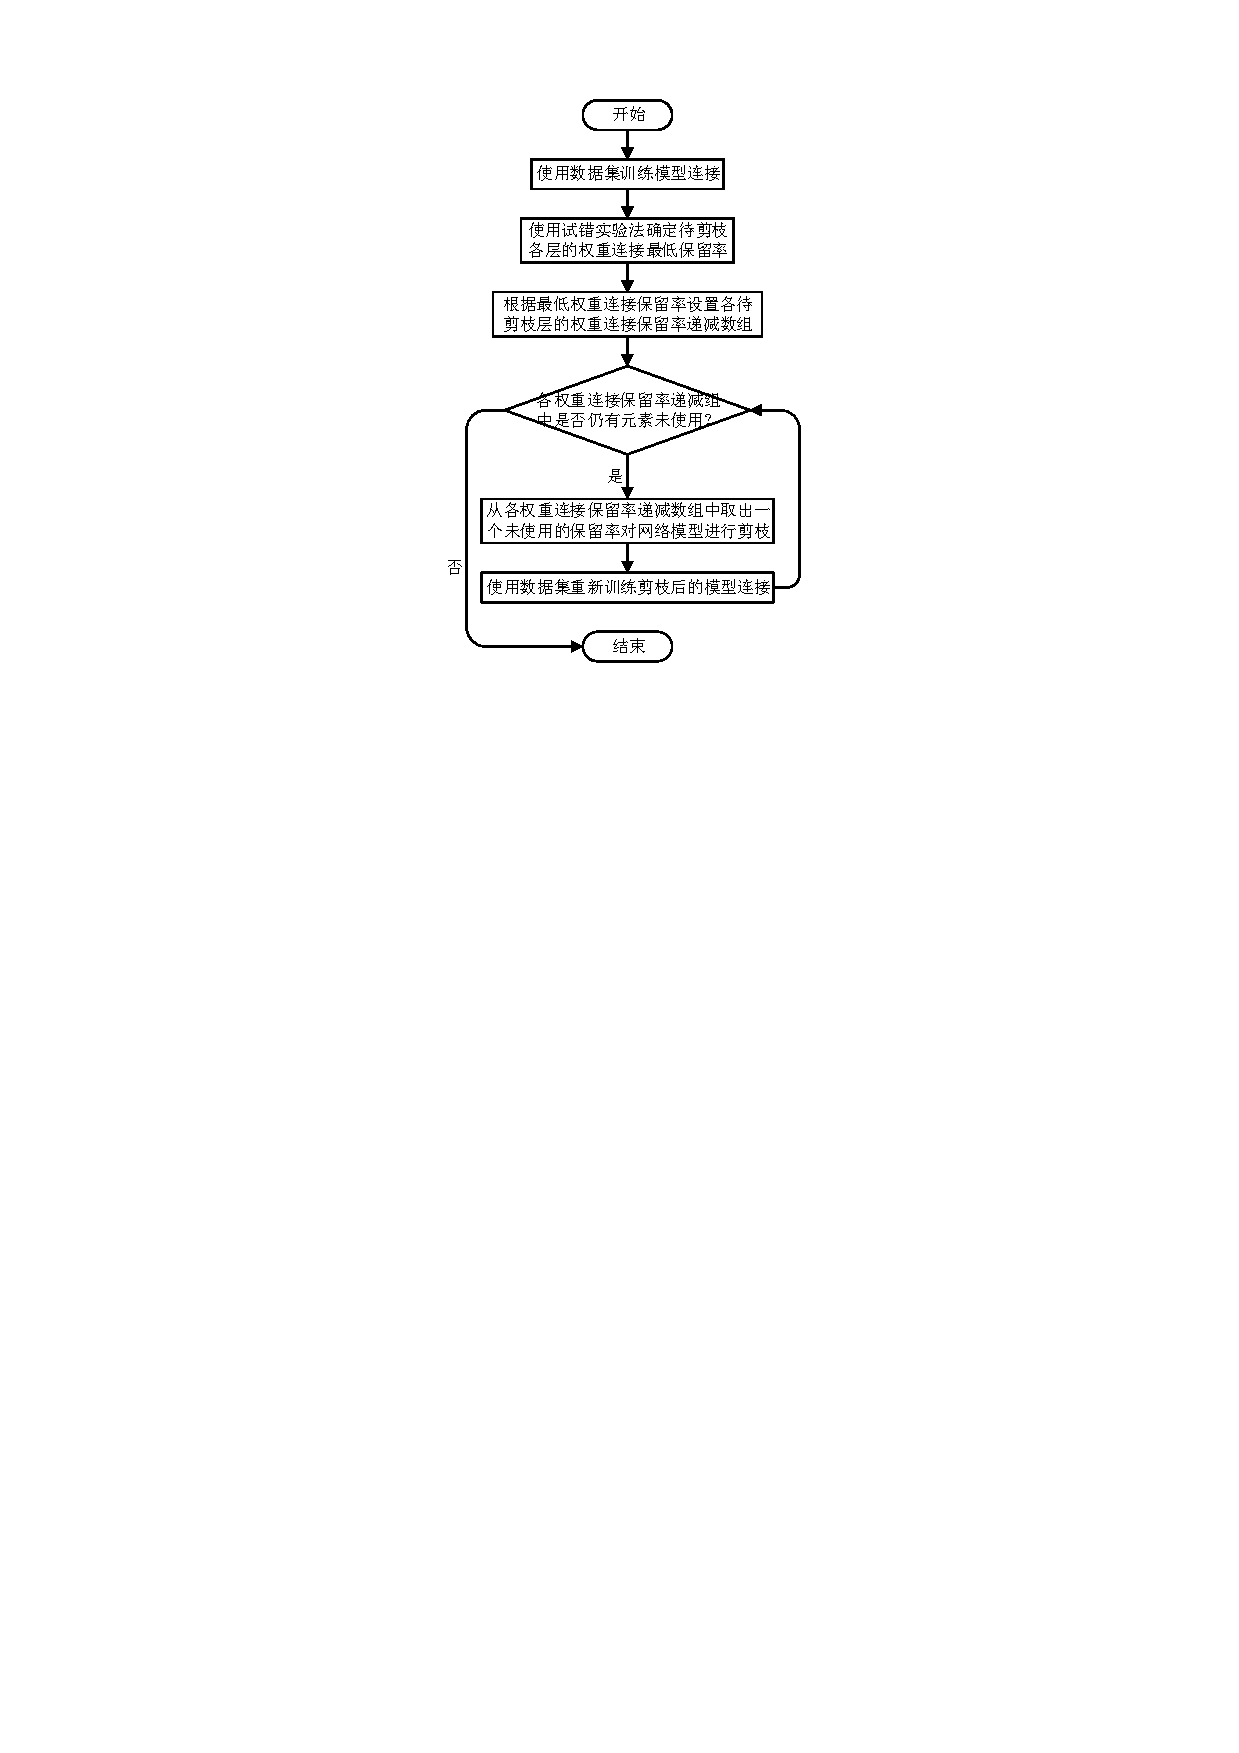
\includegraphics[height=0.8\textwidth]{figures/prune.pdf}
    \caption{“剪枝-重训”流程概览}\label{figure:figure20}
\end{figure}

图\ref{figure:figure20}描述了模型“剪枝-重训”的整体流程。首先,使用数据的训练集对CNN模型进行训练以获得稠密权重连接。接着,使用试错实验法确定各个待剪枝层的最低权重连接保留率。本文采用逐渐降低权重连接保留率的方式对网络模型进行迭代“剪枝-重训”,而不是使用最低权重连接保留率一次性对模型进行剪枝。因此,本文根据上一步得到的最低权重连接保留率来设置各待剪枝层的权重连接保留率递减数组。举例来说,对于某一层L,使用试错实验法发现将其保留率设为0.1对模型整体精度损失不大,则L层的权重连接保留率递减数组可设置成$[0.95,0.9,0.85,...,0.15,0.1]$。最后,对各待剪枝层的权重连接保留率递减数组进行迭代:每次取出一组保留率对模型进行“剪枝-重训”操作,直至各待剪枝层的权重连接达到目标保留量。

根据图\ref{figure:figure20}所描述的流程,本文对Caffe框架源码进行了改良,使其支持上述的“剪枝-重训”操作,并针对LeNet-5模型和AlexNet模型进行了实验。另外,对于稀疏矩阵,本文使用CSR格式对其进行存储,即只保存稀疏矩阵的非零值、行的范围以及非零值的列下标。

\subsection{LeNet-5模型剪枝}

图\ref{figure:figure21}显示了LeNet-5模型精确度随两个全连接层权重连接保留率的变化趋势。从趋势图上可以看出:全连接层ip1包含的冗余连接数过多,所以减少其权重连接对整个模型的前向推断精确度影响不大;而全连接层ip2受剪枝影响较大,当只保留其5\%的权重连接时会导致整个模型的推断精确度下降到82\%左右。因此,为了保证剪枝后LeNet-5模型的推断精确度仍在90\%以上,本文将全连接层ip1和ip2的最低权重连接保留率分别设为0.05和0.1。

\begin{figure}[htbp]
    \centering
    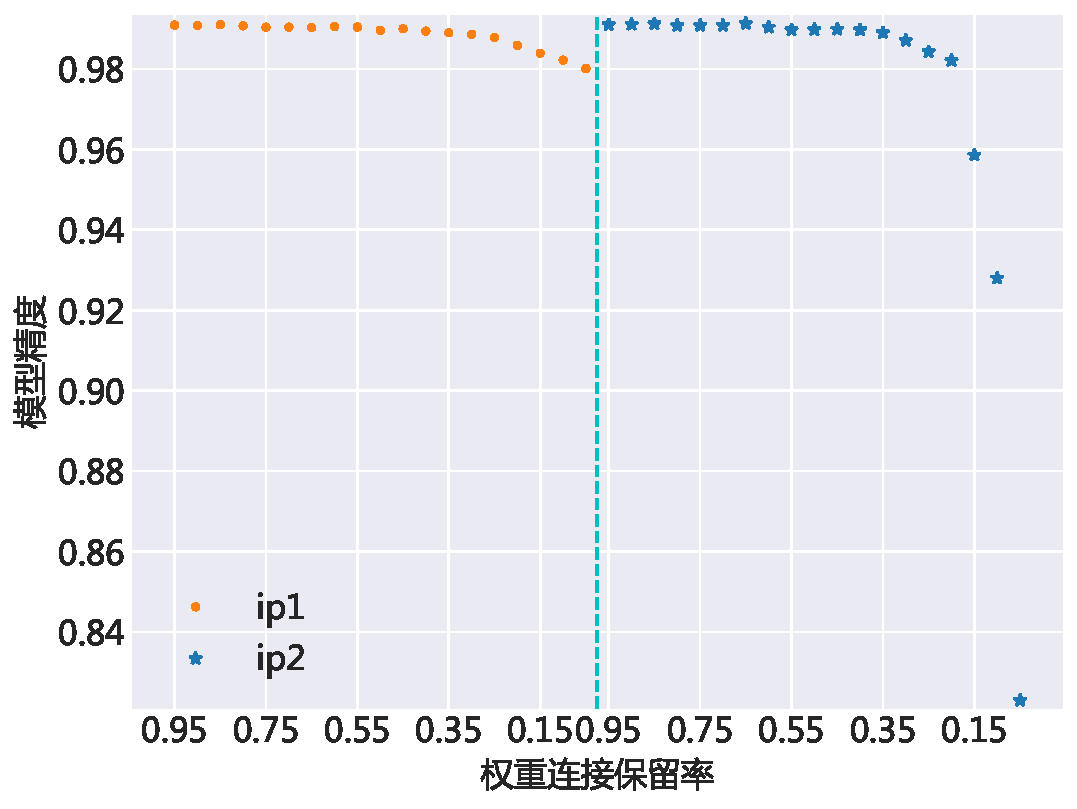
\includegraphics[height=0.45\textwidth]{figures/lenet_pruned_threshold.pdf}
    \caption{LeNet-5模型精确度随全连接层权重连接保留率的变化曲线}\label{figure:figure21}
\end{figure}

使用图\ref{figure:figure20}所示的“剪枝-重训”流程对LeNet-5模型剪枝后,可以发现其推断精确度仍可高达99.05\%,这几乎没有导致精度上任何损失。剪枝后的模型经CSR格式进行存储后,模型大小仅为原始模型的15.65\%。在此需要说明,虽然全连接层ip1和ip2的权重参数分别减少了95\%和90\%,但是CSR存储格式需要存储稀疏矩阵中所有非零值元素的两类信息(元素值和其对应的列下标),所以模型大小仅压缩到原始模型的15\%左右。由LeNet-5模型所有全连接层剪枝前后的权重分布对比图\ref{figure:figure22}可知,LeNet-5模型经剪枝后全连接层的权重只有很少一部分值为非零值,这说明剪枝操作确实将原有的稠密权重矩阵转换为了稀疏权重矩阵。

\begin{figure}[htbp]
    \centering
    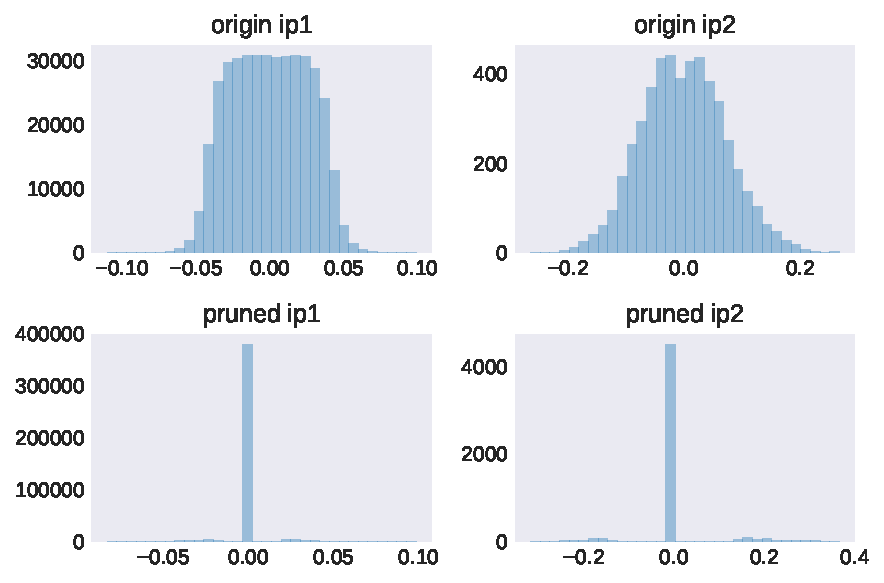
\includegraphics[height=0.45\textwidth]{figures/lenet_pruned_weights.pdf}
    \caption{LeNet-5模型全连接层剪枝前后权重分布对比}\label{figure:figure22}
\end{figure}

LeNet-5模型结构比较简单,因此其原始大小也仅1.7M,对其进行压缩意义并非很大。因此,接下来本文使用“剪枝-重训”方法对AlexNet模型进行压缩。


\subsection{AlexNet模型剪枝}

同样地,本文使用试错实验法确定AlexNet模型各全连接层的最低权重连接保留率,其模型精确度随不同层权重连接保留率的变化趋势如图\ref{figure:figure23}所示。通过对比可知,fc6层的剪枝对模型精确度影响最大,而fc8层的剪枝对模型精确度影响较小。为了保证剪枝后模型的top-1精确度仍在50\%以上,本文将全连接层fc6、fc7和fc8的最低权重连接保留率均设置成0.15。注意,本文所使用的AlexNet模型在ImageNet\cite{imagenet.org}数据集上的top-1精确度为55.78\%。

\begin{figure}[htbp]
    \centering
    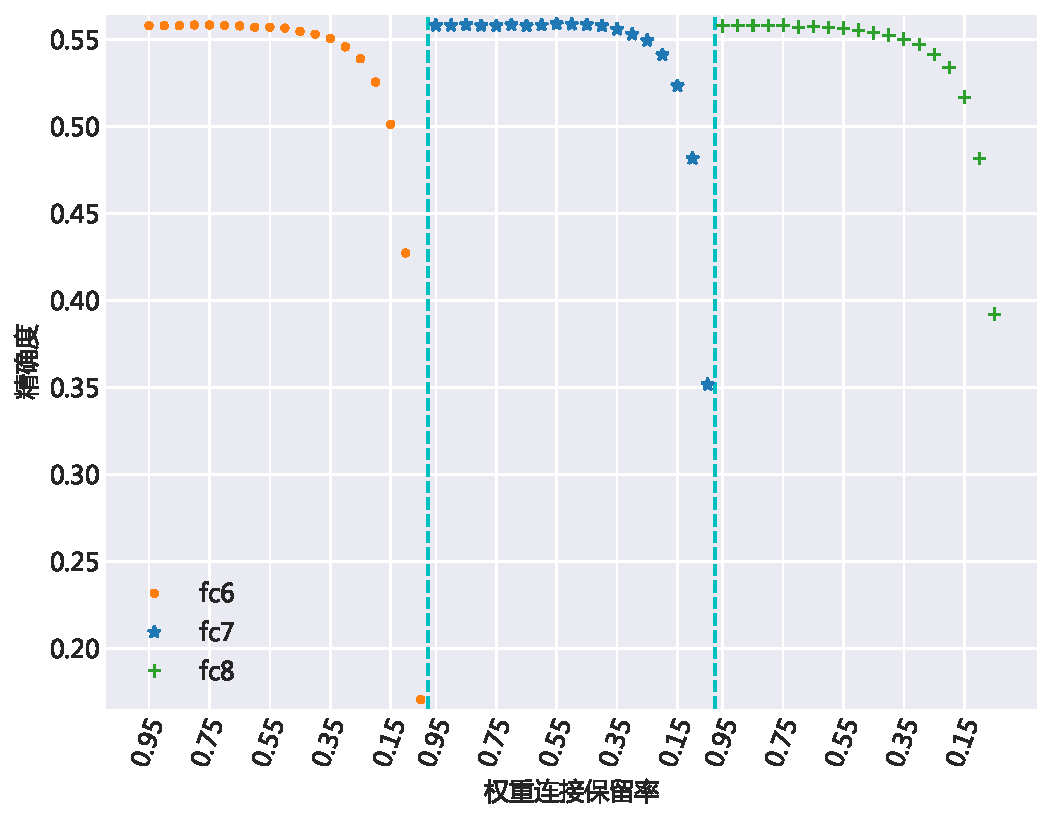
\includegraphics[height=0.45\textwidth]{figures/alexnet_pruned_threshold.pdf}
    \caption{AlexNet模型精确度随全连接层权重连接保留率的变化曲线}\label{figure:figure23}
\end{figure}

经多次“剪枝-重训”操作后,AlexNet模型的所有全连接层都仅保留了原有权重的15\%,而模型的top-1精确度变成了54.80\%,模型的精确度仅下降了0.98\%。因为实验中对每次剪枝后的模型仅仅重新训练了10000次,所以这可能造成了模型精确度0.98\%的损失。如果增加每次剪枝后模型的重新训练次数,模型的精确度损失就会减少。使用CSR格式对剪枝后的AlexNet模型进行存储,其模型大小约为85M,这比原始模型的250M减少了165M,仅占原始模型大小的34\%。图\ref{figure:figure24}显示了AlexNet模型的各个全连接层剪枝前后权重分布对比。从分布图中可以明显看出,经剪枝后,AlexNet模型的所有全连接层的权重值仅有很少一部分值不为0。

\begin{figure}[htbp]
    \centering
    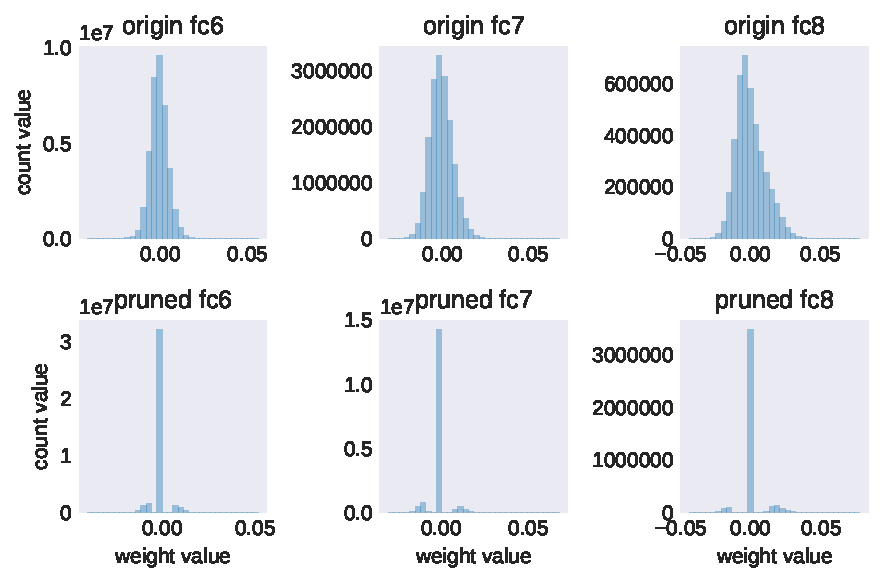
\includegraphics[height=0.45\textwidth]{figures/alexnet_pruned_weights.pdf}
    \caption{AlexNet模型全连接层剪枝前后权重分布对比}\label{figure:figure24}
\end{figure}

基于ODROID-XU3平台,本文分析比较了AlexNet模型在剪枝前后的首次加载时间、能耗和功耗变化,结果如图\ref{figure:figure27}所示。分析图\ref{figure:figure27}中的数据可知,对AlexNet模型的全连接层进行剪枝后(仅保留全连接层原有权重的15\%),模型的首次加载时间减少了60\%并且内存读取操作所产生的能耗也降为原来的一半。这说明,对神经网络模型进行剪枝操作不仅可以降低模型的内存占用还可以加快模型的加载速度并同时降低内存的能耗开销。

\begin{figure}[htbp]
    \centering
    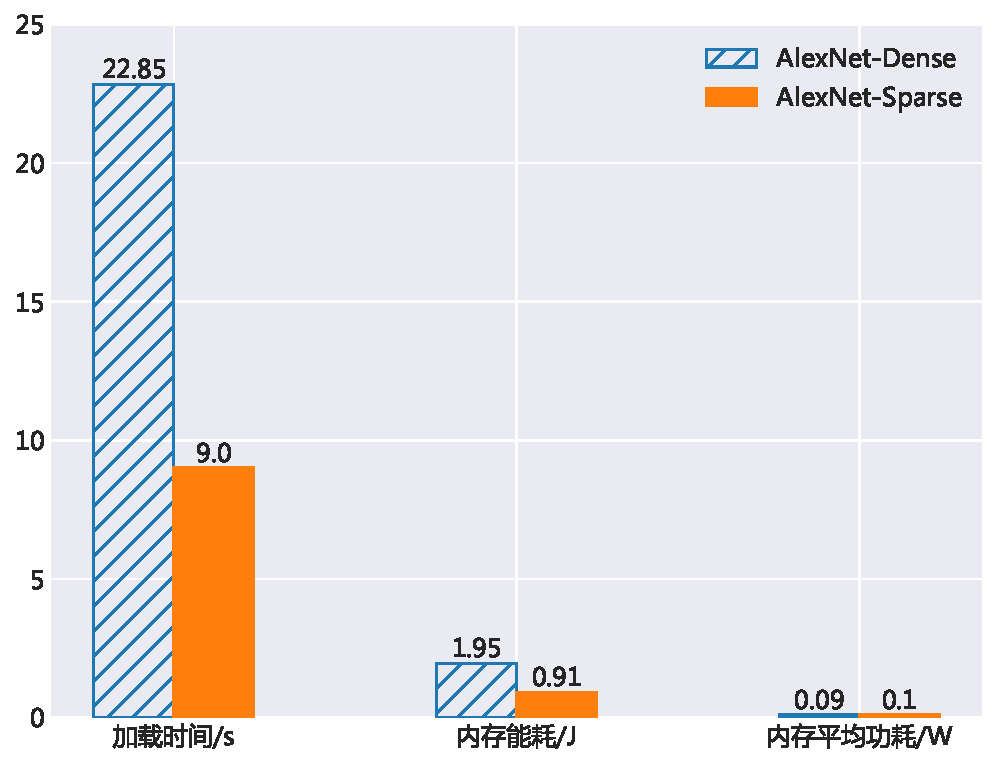
\includegraphics[height=0.4\textwidth]{figures/alexnet_init.pdf}
    \caption{剪枝前后AlexNet模型首次加载时间、能耗和功耗对比}\label{figure:figure27}
\end{figure}

\subsection{手机端SpMV的实现}

对于剪枝压缩后的卷积神经网络模型,本文使用稀疏矩阵向量乘(SpMV)代替原全连接层的稠密矩阵向量乘(内积操作),对于一个使用CSR格式存储的稀疏矩阵与一个向量相乘时,其实现伪代码如算法\ref{algo:algorithm7}所示。

\begin{algorithm}[htbp]
  \small
  \SetAlgoLined
  \KwData{num\_rows, ptr, indices, data, bias, vec, out}
    \begin{spacing}{0.9}
    num\_rows表示稀疏矩阵的总行数\;
    ptr, indices, data分别表示行的范围、非零值的列下标以及稀疏矩阵的非零值\;
    bias, vec, out分别表示偏置矩阵、乘数向量以及乘积结果\;
  \For{row in 0 ... num\_rows-1}{
        tmp = 0\;
        计算第row行的非零值下标范围[start\_row, end\_row)\;
        \For{j in start\_row ... end\_row-1}{
            temp += data[j] * vec[indices[j]];
        }
        out[row] = temp + bias[row];
  }
    \end{spacing}
  \caption{SpMV的实现伪代码}
  \label{algo:algorithm7}
\end{algorithm}

根据算法\ref{algo:algorithm7}所述过程,本文分别于手机GPU和CPU上实现了稀疏矩阵向量乘操作。图\ref{figure:figure25}显示了于ODROID-XU3平台的GPU和CPU上进行稀疏矩阵向量乘和使用内积进行稠密矩阵向量乘的运行时间、能耗和功耗对比。实验中,矩阵维度为$4096 \times 9216$,向量维度为$9216 \times 1$,矩阵的非零值比重为15\%。

\begin{figure}[htbp]
    \centering
    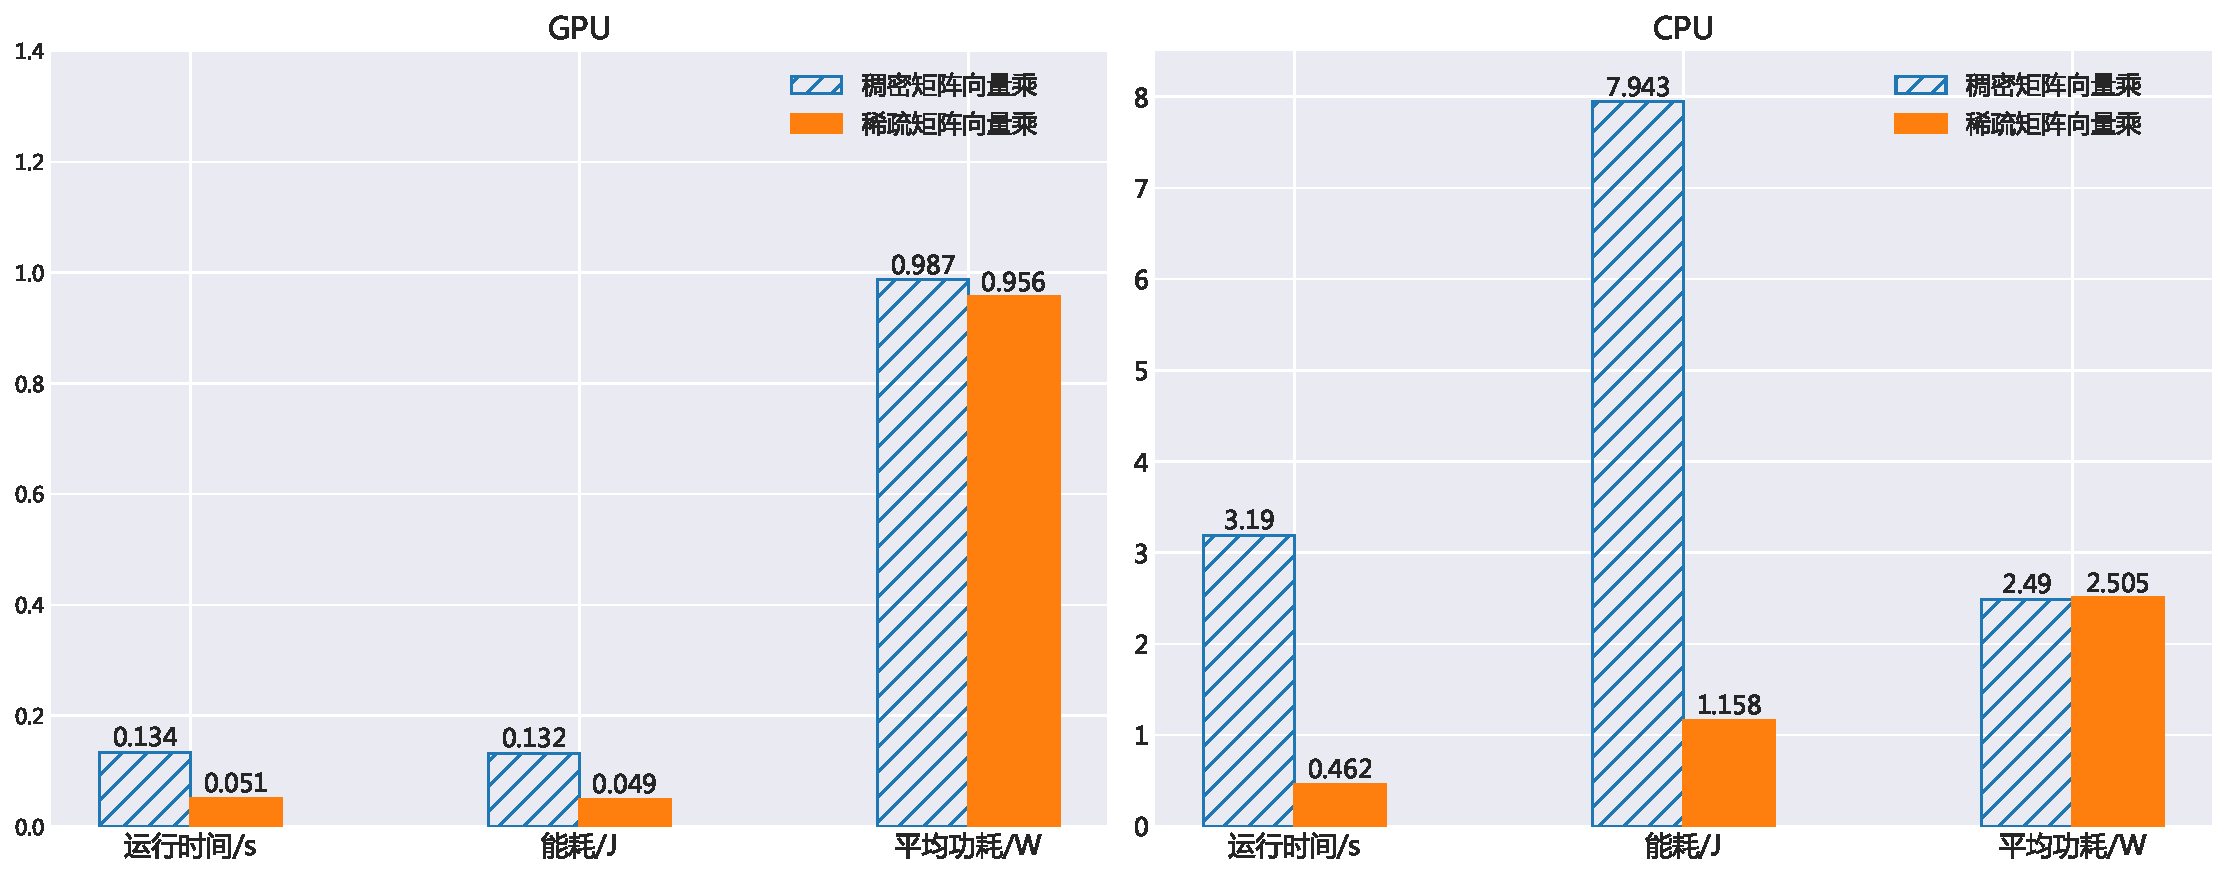
\includegraphics[width=1.0\textwidth]{figures/spmv.pdf}
    \caption{稠密矩阵向量乘和稀疏矩阵向量乘的运行时间、能耗和功耗对比}\label{figure:figure25}
\end{figure}

由图\ref{figure:figure25}可知,GPU上使用SpMV代替内积运算,可将矩阵向量乘操作的运行速度提升2.61倍,并且完成操作也只需原能耗的1/3左右。而在CPU上使用SpMV操作更可将运行时间和能耗均降为原来的1/7左右。这充分说明矩阵的压缩操作不仅可以带来内存占用的降低,更可以提升矩阵计算速度并同时降低能耗。


\begin{figure}[htbp]
    \centering
    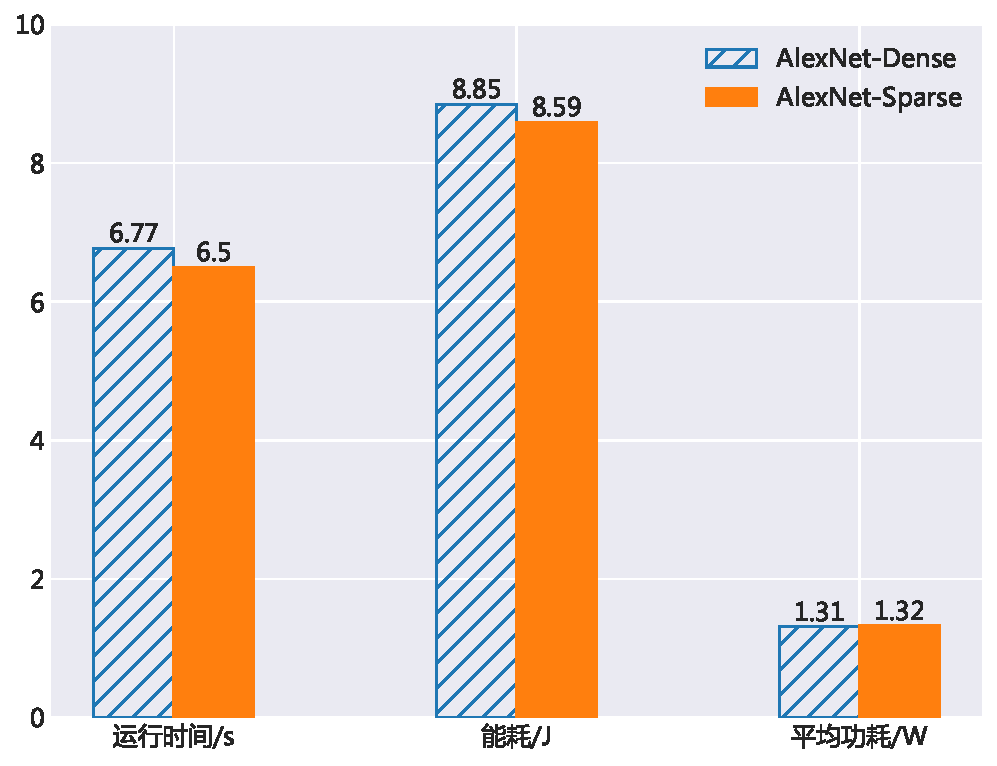
\includegraphics[height=0.4\textwidth]{figures/alexnet_sparse.pdf}
    \caption{AlexNet模型剪枝前后单张图片推断运行时间、能耗和功耗对比}\label{figure:figure26}
\end{figure}

对AlexNet模型全连接层进行剪枝并使用SpMV代替全连接层的内积算子后,再次测量其推断单张图片的运行时间、能耗和功耗如图\ref{figure:figure26}的AlexNet-Sparse数据系列所示。与剪枝前稠密的AlexNet模型相比,稀疏的AlexNet模型的前向推断时间、能耗都有所降低,但降低幅度不大。分析其原因可知,因为全连接层的计算时间占整个卷积神经网络模型的执行时间比重较小,所以使用SpMV带来的推断性能提升并不明显。

\section{本章小结}

本章主要介绍了基于手机GPU编程和模型压缩的卷积神经网络前向推断过程的能效优化方法。3.1节对CNN模型前向推断过程中所使用的基本算子进行了分解与手机端的实现,并基于ODROID-XU3平台分析比较了各个基本算子在手机GPU和CPU上的运行时能效。3.2节使用已实现的各种基本算子在手机端重构了LeNet-5模型和AlexNet模型,并分析了两个模型于手机GPU和CPU上进行单张图片推断时的能效。3.3节介绍了“剪枝-重训”的模型压缩方法,并实现了对卷积神经网络全连接层权重的压缩。通过对LeNet-5和AlexNet两个模型的剪枝操作,本文验证了使用压缩方法提升CNN模型于手机端运行时能效的有效性。最后,基于压缩后的稀疏网络模型,本文使用稀疏矩阵向量乘操作(SpMV)代替全连接层的内积操作,进一步分析了压缩所带来的性能提升。截至本章,本文已经开发了一套可以分别于手机GPU和CPU上运行的CNN推断时库,该库还通过SpMV操作支持经“剪枝-重训”压缩处理的稀疏CNN模型。

\cleardoublepage

\chapter{基于异构计算的自适应计算任务分配}
\label{chapter:chapter4}

本章首先探讨了移动端SoC的发展趋势及其对深度学习模型于移动端进行离线推断的影响。\ref{chapter:chapter4-2}节通过对比分析CNN前向推断于手机GPU和CPU上的执行能效详细阐述了使用移动设备上所有可获得的本地异构处理器运行CNN模型推断并非是一种高能效的方式。\ref{chapter:chapter4-3-1}节提出了一种无需人为干预、可自适应计算目标移动平台上所有本地处理器能效的算法。使用该算法可进一步获得目标移动平台上可用于执行CNN前向推断的高能效设备处理器组合。\ref{chapter:chapter4-3-2}节给出了一种为所选择设备处理器组合分配计算任务的方法。\ref{chapter:chapter4-4}节基于ODROID-XU3平台实现了本文所提出的算法,并验证了这些算法的有效性。

\section{移动端SoC的发展趋势}
\label{chapter:chapter4-1}
多核异构CPUs(如,ARM的big.LITTLE\cite{chung2012heterogeneous})已然成为当前移动设备处理器的主流架构,而GPUs也已集成到绝大部分的移动设备中。GPUs与生俱来的并行计算能力很适合用来处理深度模型中的常见计算类型。然而,处理能力较强的GPUs也会以惊人的速度消耗着移动设备电池电量。事实上,手机GPUs的设计过程中更加重视的是低功耗而不是高性能,所以当前商业上应用的大多数移动GPUs的计算能力并不是很强大,如Mali™-T628 MP6的频率仅为600MHz、核心数仅为6。因此,单独的GPUs解决方案也不能够满足移动平台上深度学习模型的运行条件。除GPUs外,我们还应该注意到,移动设备中也集成了一些低功耗处理器,如DSPs、LPUs、NPUs等。高通骁龙系列的SoC集成了Hexagon DSP;英伟达的Tegra K1 SoC除了提供了高性能的GPU(192核)、2.3Ghz的4核CPU外,还提供了一个第五代低功耗核LPC;华为的海思麒麟970还内置了神经网络处理单元(NPUs),使用NPU可进行高效的 AI相关计算。另外,英伟达如今已跟芯片设计公司ARM达成合作,将开源的NVIDIA深度学习加速器(NVDLA)架构集成到Arm的Project Trillium平台上,从而更好地实现移动端机器学习。在2018年的世界移动通信大会(MWC)上,联发科也宣布推出Helio P60芯片,该芯片使用的ARM Cortex™-A73大核心是专为手机端AI应用设计的处理器架构,可用于实现深度学习面部检测、物体与场景辨识等功能。可以看出,移动端SoC芯片将会越来越多地配备不同用途的专用处理器,并且每一种处理器都拥有着不同的资源特征。

根据层的类型和其他方面的模型特征,使用不同的处理器组合执行不同深度学习模型,这样便可以带来不同的性能-功耗折中。因此,如何高效地利用手机本地各种异构处理器将是移除深度学习模型被嵌入式平台所广泛采用之屏障的关键\cite{attia2015dynamic}。

\section{基于异构计算的CNN推断研究动机}
\label{chapter:chapter4-2}
之前的研究工作要么在CNN推断中没有很好地利用手机移动设备的异构计算能力(如仅使用CPU或GPU进行前向推断),要么总是试图利用所有可获得的本地设备进行模型推断,而本章主要探索如何高能效地使用手机移动设备的异构计算能力完成CNN模型的离线推断过程。

\begin{figure}[htbp]
    \centering
    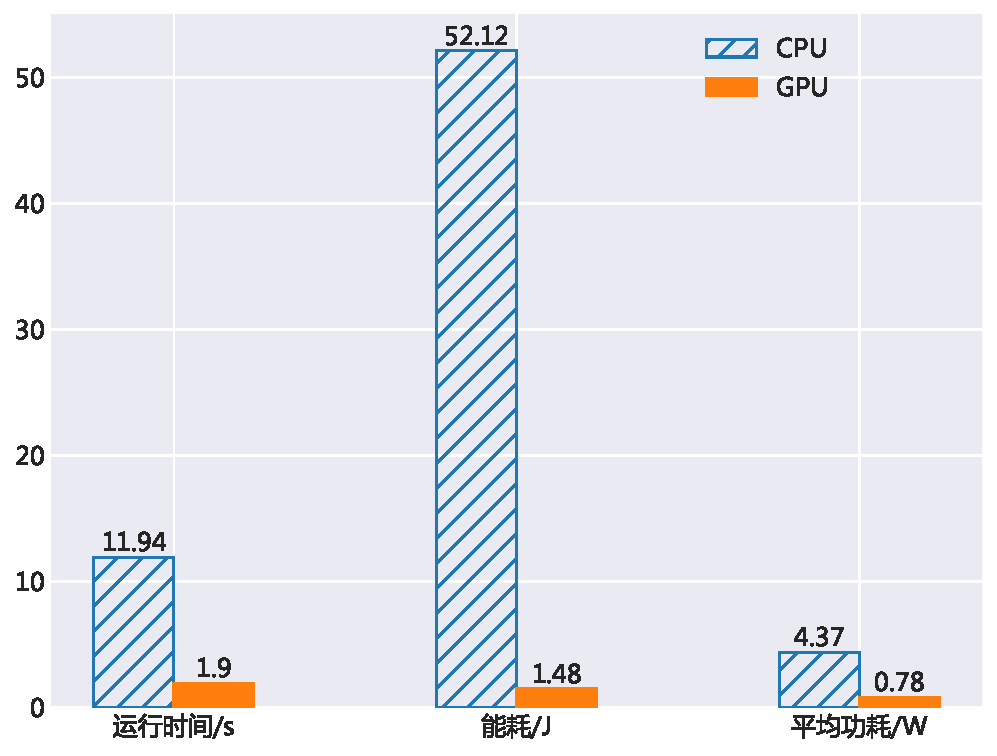
\includegraphics[height=0.4\textwidth]{figures/yolo_energy.pdf}
    \caption{手机GPU和CPU执行一次完整CNN推断的运行时间、能耗和功耗}\label{figure:figure28}
\end{figure}

图\ref{figure:figure28}显示了分别于手机GPU和CPU上运行一次完整CNN推断所需时间、能耗和功耗。为了充分利用手机CPU的计算性能,在CPU上执行CNN前向推断时使用了ARM处理器提供的NEON指令(一种单指令多数据流)并且启用了与处理器核心数相同的线程。由图\ref{figure:figure28}可知,即使利用了CPU所有的并行处理能力,CPU执行一次完整的CNN前向推断过程仍需要耗时11.94秒、耗能52.12焦。然而,当使用GPU去处理相同的一次推断时,平均运行时间和能耗仅为1.9秒和1.48焦。由此可见,若同时使用手机GPU和CPU并行地执行CNN的前向推断过程,其执行时间肯定会有所降低,但是其能效可能就会很低。原因可以由表\ref{table:table9}所示的EDP能效值得出,其中GPU的推断能效是CPU的221倍。因为手机的电池电量总是有限的,所以手机系统必须为计算过程维持一个较好的执行速度与能耗开销的折中。

\begin{table}[htbp]
  \centering
  \caption{分别于手机GPU和CPU上执行一次完整CNN推断的能效}
  \label{table:table9}
  \begin{tabular}{cc}
    \toprule
      运行处理器 & EDP(Joules*seconds) \\
    \midrule
      CPU & 622.31 \\
      GPU & 2.81 \\
    \bottomrule
  \end{tabular}
\end{table}

基于上述分析,本文得出结论:手机移动平台需要使用一个高能效的本地异构设备处理器组合而非简单地利用所有可获得的异构计算处理器去执行CNN的前向推断过程。

\section{基于异构计算的自适应计算任务分配策略}

图\ref{figure:figure29}显示了基于异构计算的自适应计算任务分配策略的基本流程。首先,为了在目标移动平台上寻找一个可高能效并行执行CNN前向推断的异构设备处理器组合,手机应用的CNN运行时库会根据第\ref{chapter:chapter4-3-1}章节提出的算法自动测量本地所有不同设备处理器的能效。然后,一旦寻找到所需的设备处理器组合,CNN运行时库会根据所选择的每一个处理器的性能对计算任务进行划分,划分方法详见第\ref{chapter:chapter4-3-2}章节。最后,所有的计算任务会被所选择的高能效设备处理器组合同时处理。

\begin{figure}[htbp]
    \centering
    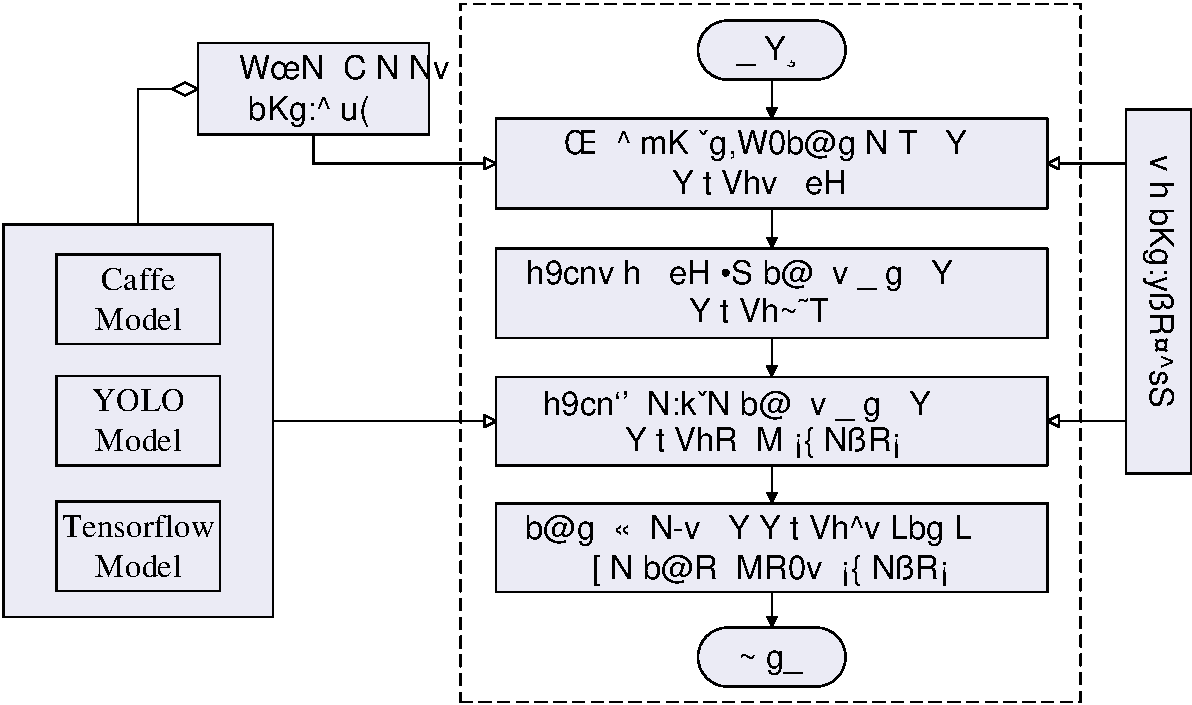
\includegraphics[height=0.4\textwidth]{figures/strategy_overview.pdf}
    \caption{基于异构计算的自适应计算任务分配策略概览}\label{figure:figure29}
\end{figure}

\subsection{高能效设备处理器组合的搜索}
\label{chapter:chapter4-3-1}

为了获得所期望的高能效设备处理器组合,首先需要了解目标手机移动平台上每一个可访问设备处理器的能效值。本文使用一种简单有效的方法来刻画目标平台上所有设备处理器的性能和能耗。简单来说,若目标平台上所有可访问的设备处理器数量为$n$,则在CNN推断时库的前$n$次运行中,每次都仅使用一个可访问的设备处理器执行完整的CNN推断。在每次执行完CNN推断后,推断过程在该设备上所需的执行时间、能耗、平均功耗以及EDP能效值会被记录下来。这一步会造成一些运行时开销,但是它仅仅发生在程序的前若干次运行中,因此这些开销会被程序的整个运行周期所均摊。接下来,为了给设备处理器选择操作做准备,每一个本地设备处理器的性能和功耗将会被正则化。最后,根据所期望的能效值不断剔除较低能效的设备处理器便可获得所需的高能效设备处理器组合。这里需要说明一点,对于同一应用,高能效设备处理器组合可被重复使用,因此整个搜索过程仅需执行一次。

\begin{algorithm}[htbp]
  \small
  \SetAlgoLined
    \begin{spacing}{0.8}
    \KwIn{(i) CNN模型结构参数和预训练的模型权重矩阵\;
          (ii) 能效阈值$EDP_{TH}$(默认值为1)。}
    \KwOut{所期望的高能效处理器组合$S_{HC}$以及组合中所有处理器的相对性能集$Perf$。}
    遍历目标平台上所有可访问的异构设备处理器(如GPUs,CPUs,NPUs等)并将它们放入设备集合$S_{HC}$中\;
    \For{$processor_i$ \textbf{in} $S_{HC}$} {
        使用处理器$processor_i$执行一次完整的CNN推断\;
        将本次推断的执行时间$t_i$, 能耗$e_i$以及平均功耗$p_i$分别存储到$T$,$E$和$P$三个数组中\;
        使用公式\ref{equation:equation1}计算本次推断的能效$EDP_i$并将其存储在$EDP$数组中\;
    }
    找出具有最小推断执行时间的处理器$processor_{min}$\;
    将$processor_{min}$的执行时间和平均功耗分别标记为$t_{min}$和$p_{ref}$\;
    \For{$(t_i$ \textbf{in} $T)$ \textbf{and} $(p_i$ \textbf{in} $P)$} {
    计算相对性能: $perf_{ri} = \frac{t_{min}}{t_i}$,将$perf_{ri}$添加到数组$Perf$中\;
    计算相对功耗:$p_{ri} = \frac{p_{i}}{p_{ref}}$,将$p_{ri}$添加到数组$P_r$中\;
    }
    \Repeat{$edp_r < EDP_{TH}$}{
        计算相对执行时间:$t_r=\frac{1}{\sum_{perf \in Perf}perf}$\;
        计算相对总功耗:$p_{tr}={\sum_{pr \in P_r}pr}$\;
        计算相对能效EDP值:$edp_r=(p_{tr}*t_r)*t_r$\;
        \If{$edp_r \geq EDP_{TH}$}{
            找出具有最大EDP值的处理器,并记录其下标$i$\;
            从$S_{HC}$中移除$processor_i$\;
            从$Perf$中移除$perf_{ri}$\;
            从$P_r$中移除$p_{ri}$\;
        }
    }
    \textbf{return} $S_{HC}$和$Perf$\;
   \end{spacing}
  \caption{高能效设备处理器组合的搜索过程}
  \label{algo:algorithm8}
\end{algorithm}

算法\ref{algo:algorithm8}描述了在目标手机移动平台上进行高能效设备处理器组合搜索的核心过程。为了在手机本地端完成CNN前向推断过程,模型结构参数和权重矩阵的获取是必须的,这可以通过第\ref{chapter:chapter321}章节提供的模型权重参数解析脚本实现。因为算法中使用了正则化处理,所以默认的能效阈值$EDP_{TH}$设置为1。当然,用户也可以根据需要配置$EDP_{TH}$的值以得到不同的能效折中。

如算法\ref{algo:algorithm8}所示,CNN推断时库首先会遍历目标平台上所有可访问的异构设备处理器,如CPUs、GPUs或NPUs等。然后,所有可获得的设备处理器被收集到一个容器中,这是整个搜索过程的初始化步骤(行1)。使用本文提出的策略,用户不需要提前测量不同设备处理器的性能和功耗。这是因为CNN推断时库在它的前几次执行中会主动对每一个可获得设备处理器的性能和功耗进行评估并进一步计算出它们的能效EDP值(行2-7)。例如,如果目标手机平台上配备有CPUs、GPUs和DSPs,那么每个设备处理器都会完整地运行一次CNN推断并且它们的执行性能和功耗等信息都将被记录下来。这个方法也可以扩展应用到新的设备处理器上,如NPUs、DianNaos\cite{chen2014diannao}等。接着,拥有最小执行时间的处理器会被挑选出来作为一个参考(行8)。通过该参考处理器的性能和功耗信息,每一个处理器的性能和功耗将会被正则化(行9-12)。因为每个处理器CNN推断执行时间的倒数可反映它的推断执行速度,所以算法中处理器$processor_i$的相对性能可以通过公式$\frac{\frac{1}{t_i}}{\frac{1}{t_{min}}}=\frac{t_{min}}{t_i}$得到(行10)。

为了充分利用并行处理的优势,每一个设备处理器所分配到的计算任务量是通过考虑其性能进行动态调整的。由算法的第10行可知,参考处理器(拥有最小推断执行时间的处理器)的相对性能为1并且其他处理器的性能都小于1。因此,参考处理器的任务分配比可通过公式\ref{equation:equation2}进行计算:

\begin{equation}
     \label{equation:equation2}
     \begin{aligned}
        ratio_{ref}=\frac{1}{\sum_{perf \in Perf}perf}
     \end{aligned}
\end{equation}

\noindent 假定参考处理器的串行推断执行时间为$t_s$,则其并行处理时间为 $ratio_{ref} \times t_s$(进一步的讨论详见第\ref{chapter:chapter4-3-2}章节)。因为算法中使用了正则化处理,所以$t_s$可被简单地视为1。这样,整个CNN推断的相对并行处理器时间$t_r$就等于$ratio_{ref}$(行14)。显然,所选择设备处理器组合的功耗即为组合中所有处理器的功耗总和(行15)。利用上述得到的相对执行时间和功耗即可通过公式\ref{equation:equation1}计算出所选择的每一个设备处理器的相对能效EDP值$edp_r$(行16)。然后,通过比较$edp_r$与目标能效阈值$EDP_{TH}$的大小,不断更新所选择的设备处理器组合。具体来说,若当前所选择设备处理器组合的能效低于目标能效,则当前所选择组合中能效最低的设备处理器就会被剔除并且相应的性能和功耗数据集合也会被更新(行17-22);重复上述过程直至得到所需的高能效异构计算组合。最后,所选择的设备处理器组合以及它们的性能参数集会作为算法\ref{algo:algorithm8}的输出返回给CNN推断时库。


\subsection{计算任务的划分}
\label{chapter:chapter4-3-2}

在完成高能效设备处理器组合的搜索步骤之后,CNN推断时库就可以根据算法\ref{algo:algorithm8}的返回结果将计算任务分配到所选择的处理器上执行。为了最小化并行处理时间,必须将不同处理器之间的等待时间尽量缩小。因此,一个本地设备处理器所分配到的计算任务量应该与其性能成正比,这即是计算任务划分方法的核心思想。

对于一个给定的预训练CNN模型,本文将每一层的一个输出节点定义成一个计算任务。换言之,每一层的计算任务量等于该层的输出节点数。因此,卷积层中一个计算任务就是一个卷积操作,而全连接层中一个计算任务就是一个内积操作。图\ref{figure:figure30}给出了计算任务划分的概览,其中每一条红线表示一个任务划分点。

\begin{figure}[htbp]
    \centering
    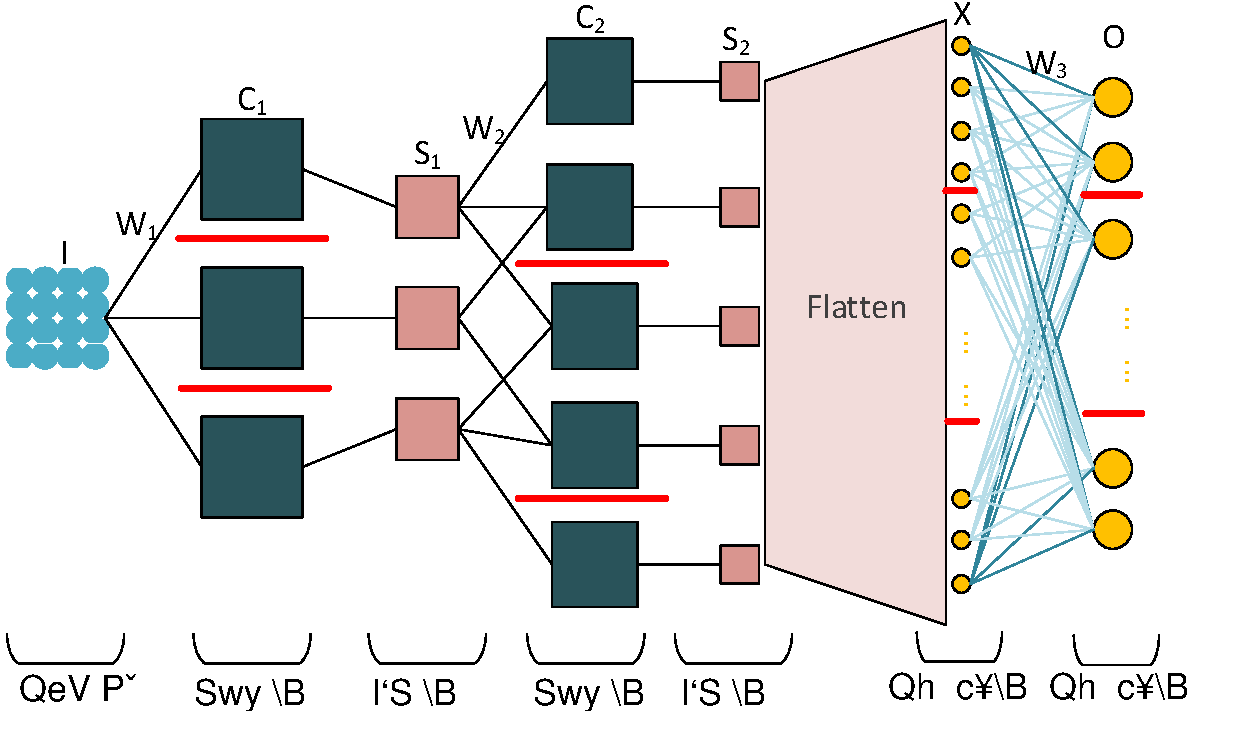
\includegraphics[height=0.4\textwidth]{figures/compute_tasks.pdf}
    \caption{计算任务划分示意图(其中每一条红线表示一个划分点)}\label{figure:figure30}
\end{figure}

算法\ref{algo:algorithm9}详细描述了为每一个所选择设备处理器计算任务分配比例的方法。如前所述,分配给每一个所选设备处理器的计算任务量取决于该处理器的性能。因此,算法\ref{algo:algorithm8}输出的相对性能参数值被用来计算每一个所选设备处理器的任务分配比例(行1-4)。接着,根据所选设备处理器的任务分配比例数组$R$,每一个设备处理器的计算任务量就可通过其任务分配比例与每一层输出节点总数的乘积计算获得。这样就可以使得性能较高的处理器就会分配到更多的计算任务而性能较低的处理器则分配到较少的计算任务,而且所有这些不同大小的计算任务几乎可以在同一时间内完成。

\begin{algorithm}[htbp]
  \small
  \SetAlgoLined
    \begin{spacing}{0.9}
    \KwIn{所选设备处理器组合中所有处理器的相对性能集$Perf$。}
    \KwOut{所选组合中处理器所分配计算任务比例集$R$。}
    \For{$perf_{i}$ \textbf{in} $Perf$} {
        计算处理器$process_i$所分配任务比例:
        $$r_i=\frac{perf_{ri}}{\sum_{perf \in Perf}perf}$$
        将$r_i$添加到数组$R$中\;
    }
    \textbf{return} $R$\;
   \end{spacing}
  \caption{设备处理器组合中每一处理器所分配任务比例的计算过程}
  \label{algo:algorithm9}
\end{algorithm}

最后,系统可以达到一个负载平衡并高能效地利用了平台提供的异构计算资源。算法\ref{algo:algorithm9}的执行开销几乎可以忽略不计,因为对于同一应用来说任务分配比例的计算只需要执行一次(任务分配比例数组可以保存到手机本地以便重复使用)。


\section{实验验证}
\label{chapter:chapter4-4}
基于第\ref{chapter:chapter3}章所开发的CNN推断时库,本章进一步实现了所提出的策略并在ODROID-XU3平台上进行了实验验证。为了充分利用CPU的并行计算能力,本章也对第\ref{chapter:chapter3}章所开发的CNN推断时库进行了优化,如在CPU版本的CNN推断过程中使用了ARM处理器提供的NEON指令并且启用了与处理器核心数相同的线程。实验中,本文将CPU和GPU的运行频率保持在某一固定值(如最大运行频率),这样可以消除设备处理器运行频率的变化对实验结果的影响。

如第\ref{chapter:chapter2-5-1}章节所述,ODROID-XU3平台上所有可获得的本地设备处理器包括一个CPU设备和两个GPU设备。因此,根据算法\ref{algo:algorithm8}和算法\ref{algo:algorithm9},CNN推断时库会得到一个高能效的设备处理器组合(这里即为ODROID-XU3平台上的两个GPU设备)。另外,实验中所考察的CNN模型主要由9个卷积层和3个全连接层构成,它们的结构参数信息如表\ref{table:table10}所示。为了说明所提策略的有效性,本文将所提策略(\emph{Energy-efficient})与贪心策略(\emph{Greedy},即总是试图使用所有可获得的异构设备处理器)进行了对比分析。

\begin{table}[htbp]
  \centering
  \caption{实验使用CNN模型的卷积层和全连接层结构参数}
  \label{table:table10}
\resizebox{1.0\textwidth}{!}{
  \begin{tabular}{ccc}
    \toprule
      名称 & 类型 & 描述\\
    \midrule
      Conv1 & 卷积层 & 输入:$3\times448\times448$,卷积核:$16\times3\times3\times3$,步长:1,padding:1,输出:$16\times448\times448$ \\
      Conv2 & 卷积层 & 输入:$16\times224\times224$,卷积核:$32\times16\times3\times3$,步长:1,padding:1,输出:$32\times224\times224$\\
      Conv3 & 卷积层 & 输入:$32\times112\times112$,卷积核:$64\times32\times3\times3$,步长:1,padding:1,输出:$64\times112\times112$ \\
      Conv4 & 卷积层 & 输入:$64\times56\times56$,卷积核:$128\times64\times3\times3$,步长:1,padding:1,输出:$128\times56\times56$\\
      Conv5 & 卷积层 & 输入:$128\times28\times28$,卷积核:$256\times128\times3\times3$,步长:1,padding:1,输出:$256\times28\times28$\\
      Conv6 & 卷积层 & 输入:$256\times14\times14$,卷积核:$512\times256\times3\times3$,步长:1,padding:1,输出:$512\times14\times14$\\
      Conv7 & 卷积层 & 输入:$512\times7\times7$,卷积核:$1024\times512\times3\times3$,步长:1,padding:1,输出:$1024\times7\times7$ \\
      Conv8 & 卷积层 & 输入:$1024\times7\times7$,卷积核:$1024\times1024\times3\times3$,步长:1,padding:1,输出:$1024\times7\times7$\\
      Conv9 & 卷积层 & 输入:$1024\times7\times7$,卷积核:$1024\times1024\times3\times3$,步长:1,padding:1,输出:$1024\times7\times7$\\
      FC10 & 全连接层 & 输入:50176, 输出:256 \\
      FC11 & 全连接层 & 输入:256, 输出:4096 \\
      FC12 & 全连接层 & 输入:4096, 输出:1470 \\
    \bottomrule
  \end{tabular}
}
\end{table}

\textbf{性能:}图\ref{figure:figure32}显示了9个卷积层和3个全连接层在ODROID-XU3平台上的执行时间。总体上来说,贪心策略的性能高于本文所提出的策略,这是因为贪心策略使用了更多的设备处理器执行计算任务。然而,贪心策略的性能提升幅度并不高,仅仅是略好于本文提出的策略,并且在全连接层上的差距非常小。这是因为GPUs的并行计算能力比使用了多线程和SIMD指令的CPUs还要强大。由此可见,使用了一个额外CPU的贪心策略在性能上并没有表现出显著的提升。从图\ref{figure:figure32}中也可以发现贪心策略中一些层的执行时间要长于本文提出的策略。这是因为贪心策略拥有更多的任务间交互开销,其在输出节点较少的层对执行时间的影响较大。

\begin{figure}[htbp]
    \centering
    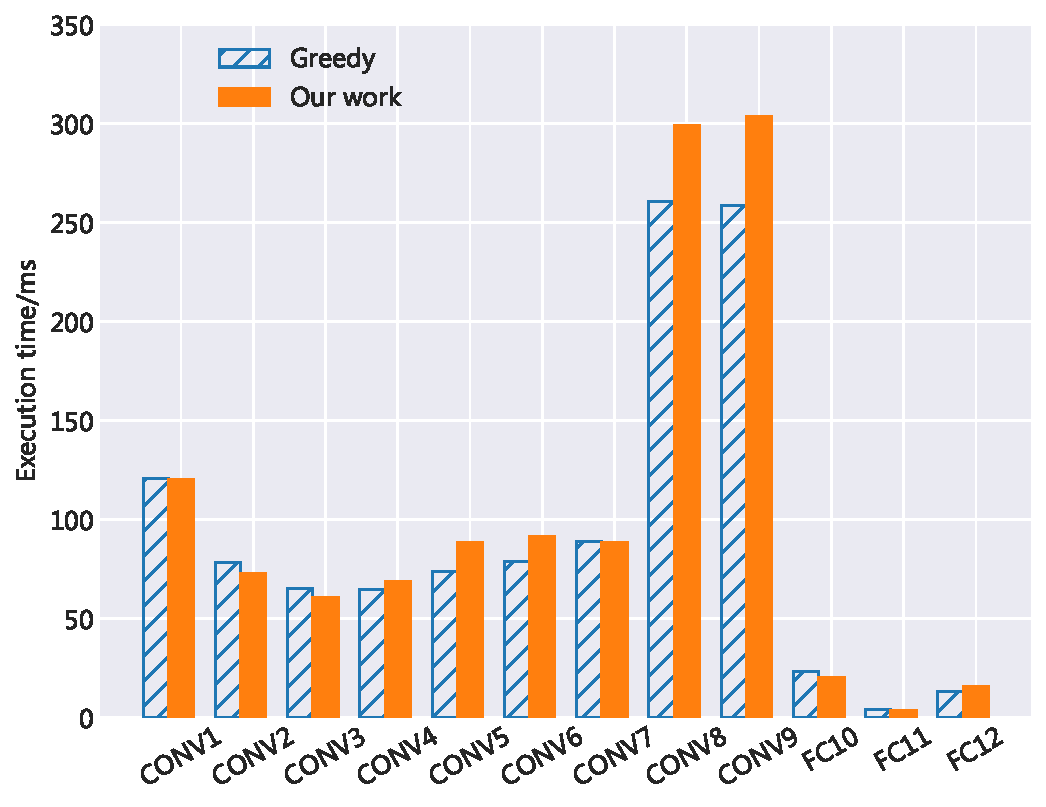
\includegraphics[height=0.4\textwidth]{figures/hc_time.pdf}
    \caption{每一层的执行时间}\label{figure:figure32}
\end{figure}

\textbf{功耗和能耗:}图\ref{figure:figure33}描述了两个策略间功耗开销的对比。整体上来看,贪心策略的平均功耗约为5.44瓦而本文所提策略的功耗约为1.22瓦。从图图\ref{figure:figure33}也可以看出,对于所有的层来说,本文所提策略的功耗要远低于贪心策略的功耗。这主要是因为移动设备GPUs在设计时更多地关注低功耗而非性能,而且通常拥有着较低的运行频率。例如,\texttt{ARM Mali-T628 MP6} GPU最大运行频率为600MHz而\texttt{Samsung Exynos5422} CPU的最大运行频率可达2GHz\cite{hardkernel.com}。

\begin{figure}[htbp]
    \centering
    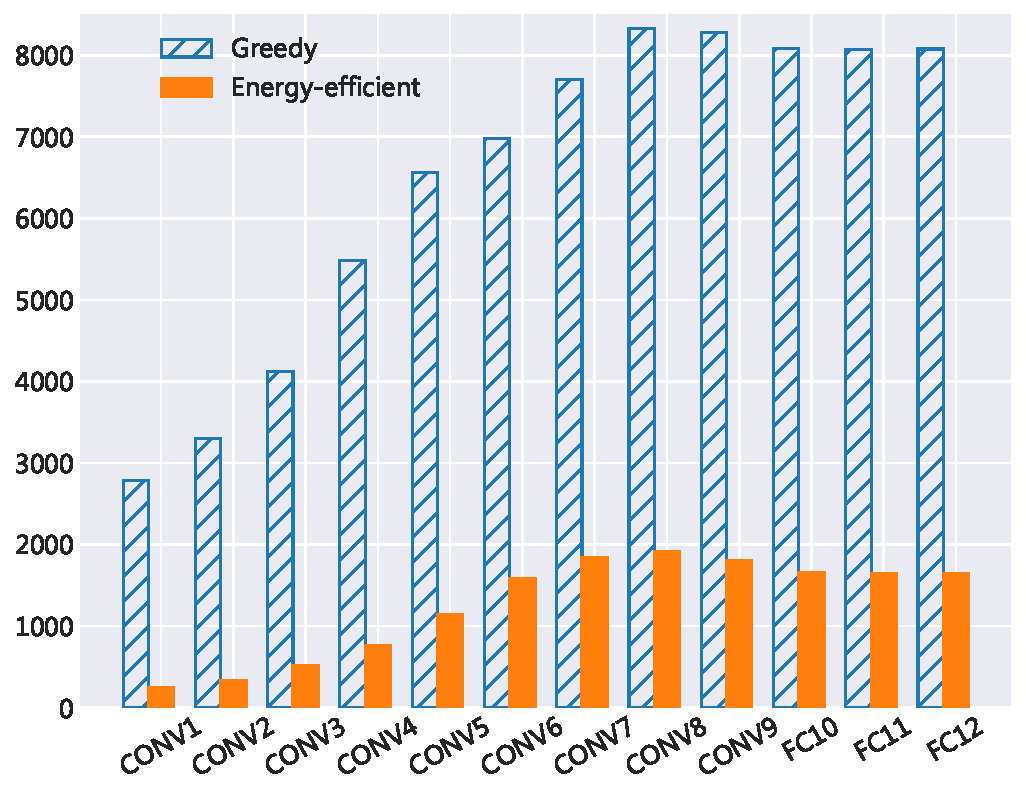
\includegraphics[height=0.4\textwidth]{figures/hc_power.pdf}
    \caption{每一层的运行时功耗}\label{figure:figure33}
\end{figure}

在各层的运行时能耗方面,图\ref{figure:figure34}显示了一个与功耗表现类似的趋势,即贪心策略的运行时能耗在各层上都要远高于本文所提出的策略。平均来说,贪心策略的运行时能耗为6.59焦而本文所提策略的能耗为1.63焦。本文所提策略通过移除一个较低能效的设备处理器有效地降低了CNN推断时的功耗和能耗。另一方面,从之前的性能分析可知,本文所提策略的推断执行性能损失很小。

\begin{figure}[htbp]
    \centering
    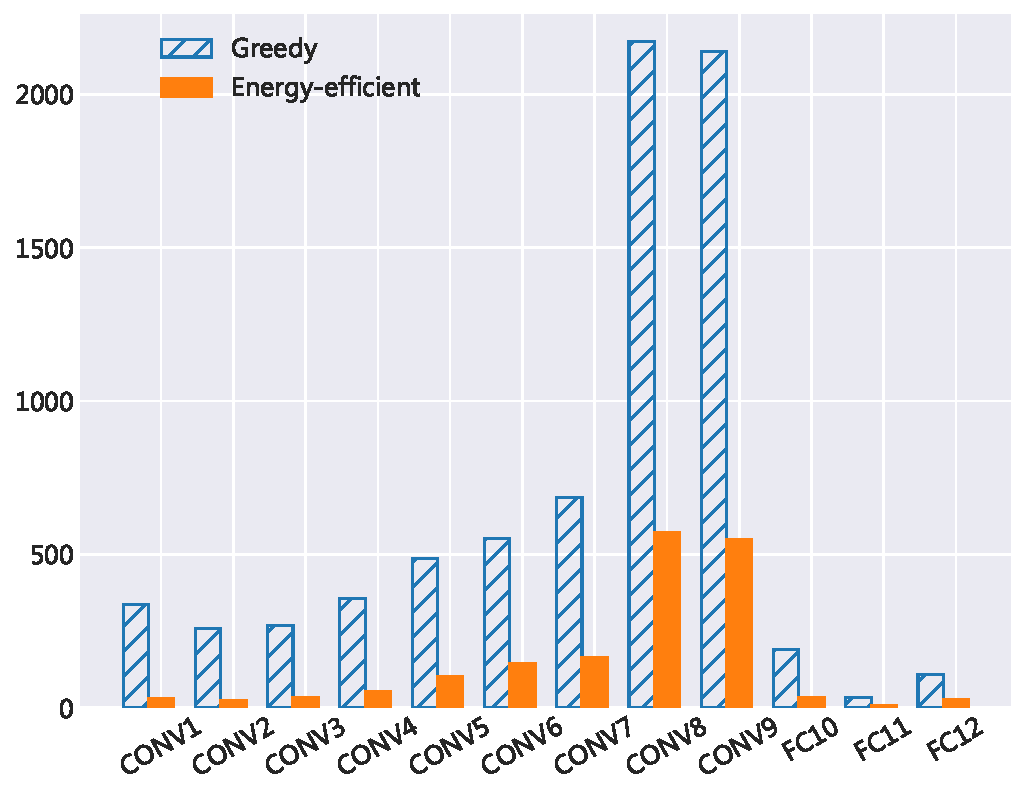
\includegraphics[height=0.4\textwidth]{figures/hc_energy.pdf}
    \caption{每一层的运行时能耗}\label{figure:figure34}
\end{figure}

\textbf{能效:}图\ref{figure:figure35}显示了不同异构计算组合执行一个完整CNN推断过程的四个方面对比,即平均运行时间、平均能耗、平均功耗和平均能效EDP值。\emph{Single GPU}仅使用一个GPU设备处理器执行CNN前向推断而\emph{Energy-efficient}使用由本文所提策略选择的两个GPU设备处理器并行执行CNN推断。\emph{Greedy}使用所有可获得的设备处理器(包含一个CPU和两个GPU设备处理器)并行执行CNN推断。从柱状图\ref{figure:figure35}可以看出,随着所使用设备处理器数量的增加,CNN推断的平均执行时间在不断降低,但是能耗和功耗随之增加。分析EDP值可知,本文所提出的策略(\emph{Energy-efficient})拥有着更好的能效,其大约是贪心策略能效的3.67倍。与此同时,本文所提出的策略在推断执行速度上仅降低了9.7\%。

\begin{figure}[htbp]
    \centering
    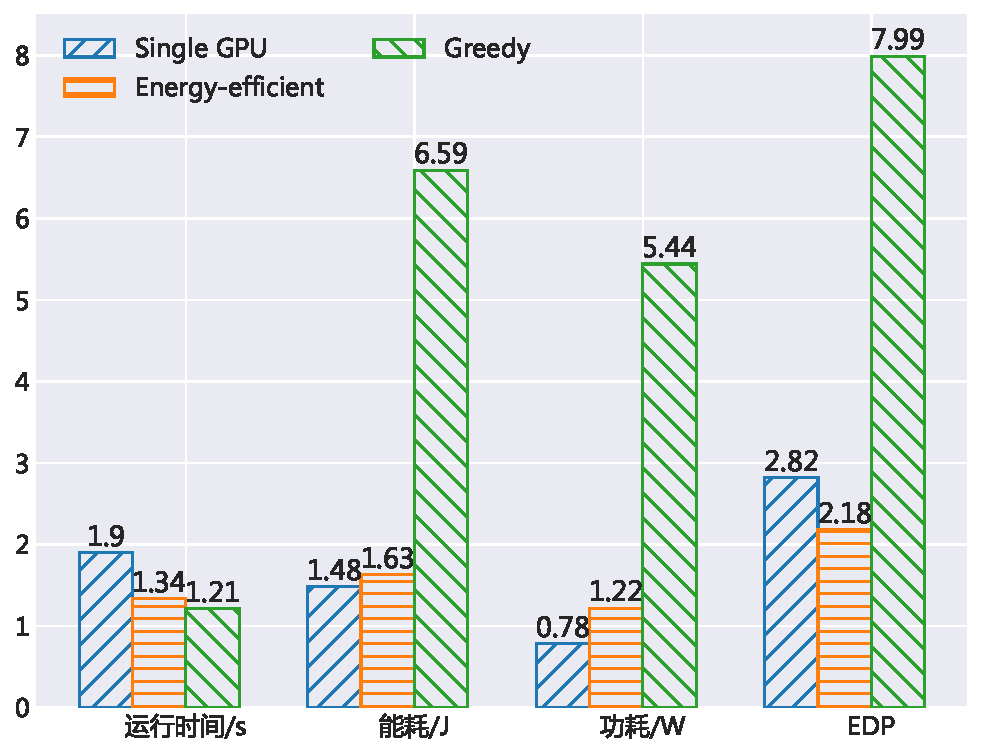
\includegraphics[height=0.4\textwidth]{figures/hc_gpu.pdf}
    \caption{不同异构计算组合的运行时间、能耗、功耗和能效对比}\label{figure:figure35}
\end{figure}

实验证明了利用所有可获得的设备处理器可以最大化加快CNN推断速度,但是这种方式也可能会导致一个非常低的推断能效。然而,对于电池容量受限的手机平台来说,除了需要关注程序的执行性能,程序执行过程中的能耗也是非常重要的\cite{brooks2000power}。

\section{本章小结}

尽管目前手机移动平台上并没有配备许多异构设备处理器,但是于手机SoC芯片上集成不同的异构处理器以执行不同的任务已然成为一种的趋势。正如第\ref{chapter:chapter4-1}章节所述,手机移动端的处理器架构在不断创新。例如,陈天石提出的DianNao在处理神经网络计算时执行速度是128-bit 2GHz SIMD处理器的117.87倍,并且功耗仅为485毫瓦\cite{chen2014diannao},其在能效上甚至超过了目前的手机GPUs。华为手机使用的麒麟970芯片即嵌入了基于DianNao架构的神经网络处理单元(NPUs)。在这种手机SoC芯片的发展趋势下,合理、高效地利用多异构设备处理器执行基于深度学习模型的手机应用将会变得越来越重要。本文对基于异构计算的手机端高能效CNN本地推断进行了探索,并对所提出的策略于ODROID-XU3平台上进行了实验验证。实验结果发现,与总是试图使用所有可获得异构设备处理器的贪心策略相比,本文所提出的策略可以获得3.67倍更高的能效而仅仅损失9.7\%的执行速度。

\cleardoublepage 
\chapter{基于应用场景的系统层能效优化}

本章首先介绍了动态电压频率调节(DVFS)的基本概念以及其在能效优化领域所发挥的作用。本章利用前述章节所实现的CNN运行时库开发了一款智能监控系统Android应用。\ref{chapter5-2}节对该应用的负载特征进行了刻画与分析,阐述了当前Android系统所采用的功耗管理器在基于深度学习模型应用上表现的不足之处。\ref{chapter5-3}节提出了一种基于应用场景的系统层能效优化策略,该策略根据应用在系统层表现的负载特征对其进行分类,这样系统便可以针对不同的应用使用不同的功耗管理策略。

\section{动态电压频率调节技术}

动态电压频率调节DVFS(Dynamic Voltage and Frequency Scaling)是一种可对芯片电压和频率进行实时动态调节的技术。当前手机CPU和GPU都支持DVFS,并且系统层也都存在着相应的功耗管理器(governor)。每一个功耗管理器都拥有一个执行频率调节的策略,并且这个策略可被配置以取得不同的能效折中。根据配置的策略,功耗管理器可以决定不同状态下的设备处理器所应该运行的频率。设备处理器的负载越高运行频率越高是这些功耗管理器所遵循的基本准则。

动态功耗\cite{benini1999policy}、短路功耗\cite{周宽久2010嵌入式软硬件低功耗优化研究综述倡}和漏电流功耗\cite{you2006compilers}是CMOS电路的三个主要功耗,因此CMOS电路的总功耗可由公式\ref{equation:equation3}表示:

\begin{equation}
     \label{equation:equation3}
     \begin{aligned}
        P = P_{Dynamic} + P_{Short} + P_{Leakage}
         = ACV^2f +  AVI_{Short} + VI_{Leakage}
     \end{aligned}
\end{equation}

式中$C$代表负载电容的容值,$V$是工作电压,$A$是当前频率下电路的平均翻转率,$f$为工作频率,$I_{Short}$和$I_{Leakage}$分别为短路电流和漏电流。从公式中可知,$C$、$V$、$A$、$f$决定了整个CMOS电路的功耗,而DVFS技术就是主要通过改变频率$f$和电压$V$的值来调节系统功耗的。


\section{智能监控系统Android应用的负载特征}
\label{chapter5-2}

基于前述章节所实现的CNN运行时库,本文开发了一款智能监控系统Android应用,其可以通过手机摄像头自动辨识周围所观察到的物体类别。图\ref{figure:figure31}显示了两张该应用的运行界面。智能监控系统应用的智能识别功能是由卷积神经网络Tiny YOLO\cite{pjreddie.com}卷积模型提供的。

\begin{figure}[htbp]
    \centering
    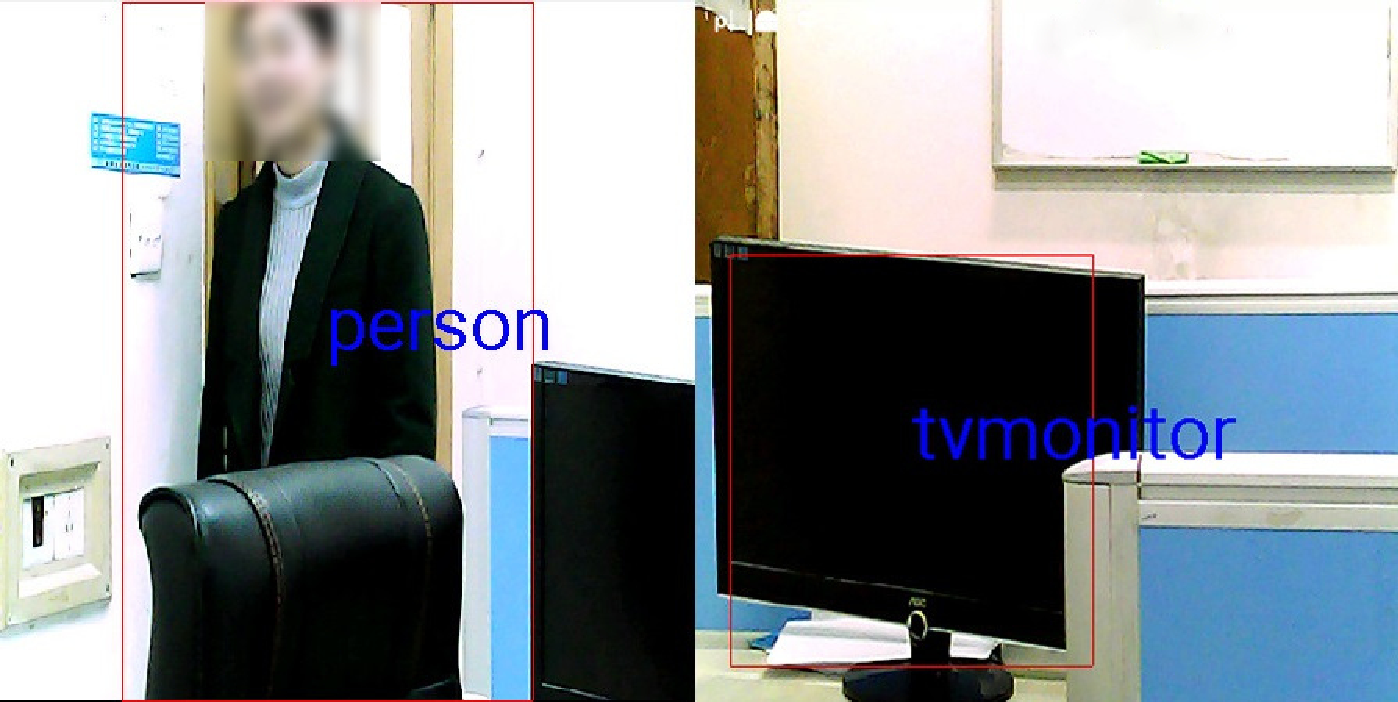
\includegraphics[height=0.4\textwidth]{figures/app.pdf}
    \caption{智能监控系统Android应用}\label{figure:figure31}
\end{figure}

图\ref{figure:figure36}显示了智能监控系统Android应用的工作流程。在智能监控系统APP启动后,它会不断地通过手机摄像头感知周围的场景。当读取到摄像头所拍摄视频中的一帧数据后,该APP会立即将该帧数据作为CNN模型的输入并执行网络的前向推断过程。推断完成后,侦测结果会在视频框中显示出来。紧接着,监控APP会立即获取下一帧图像数据并重复上述过程。

\begin{figure}[htbp]
    \centering
    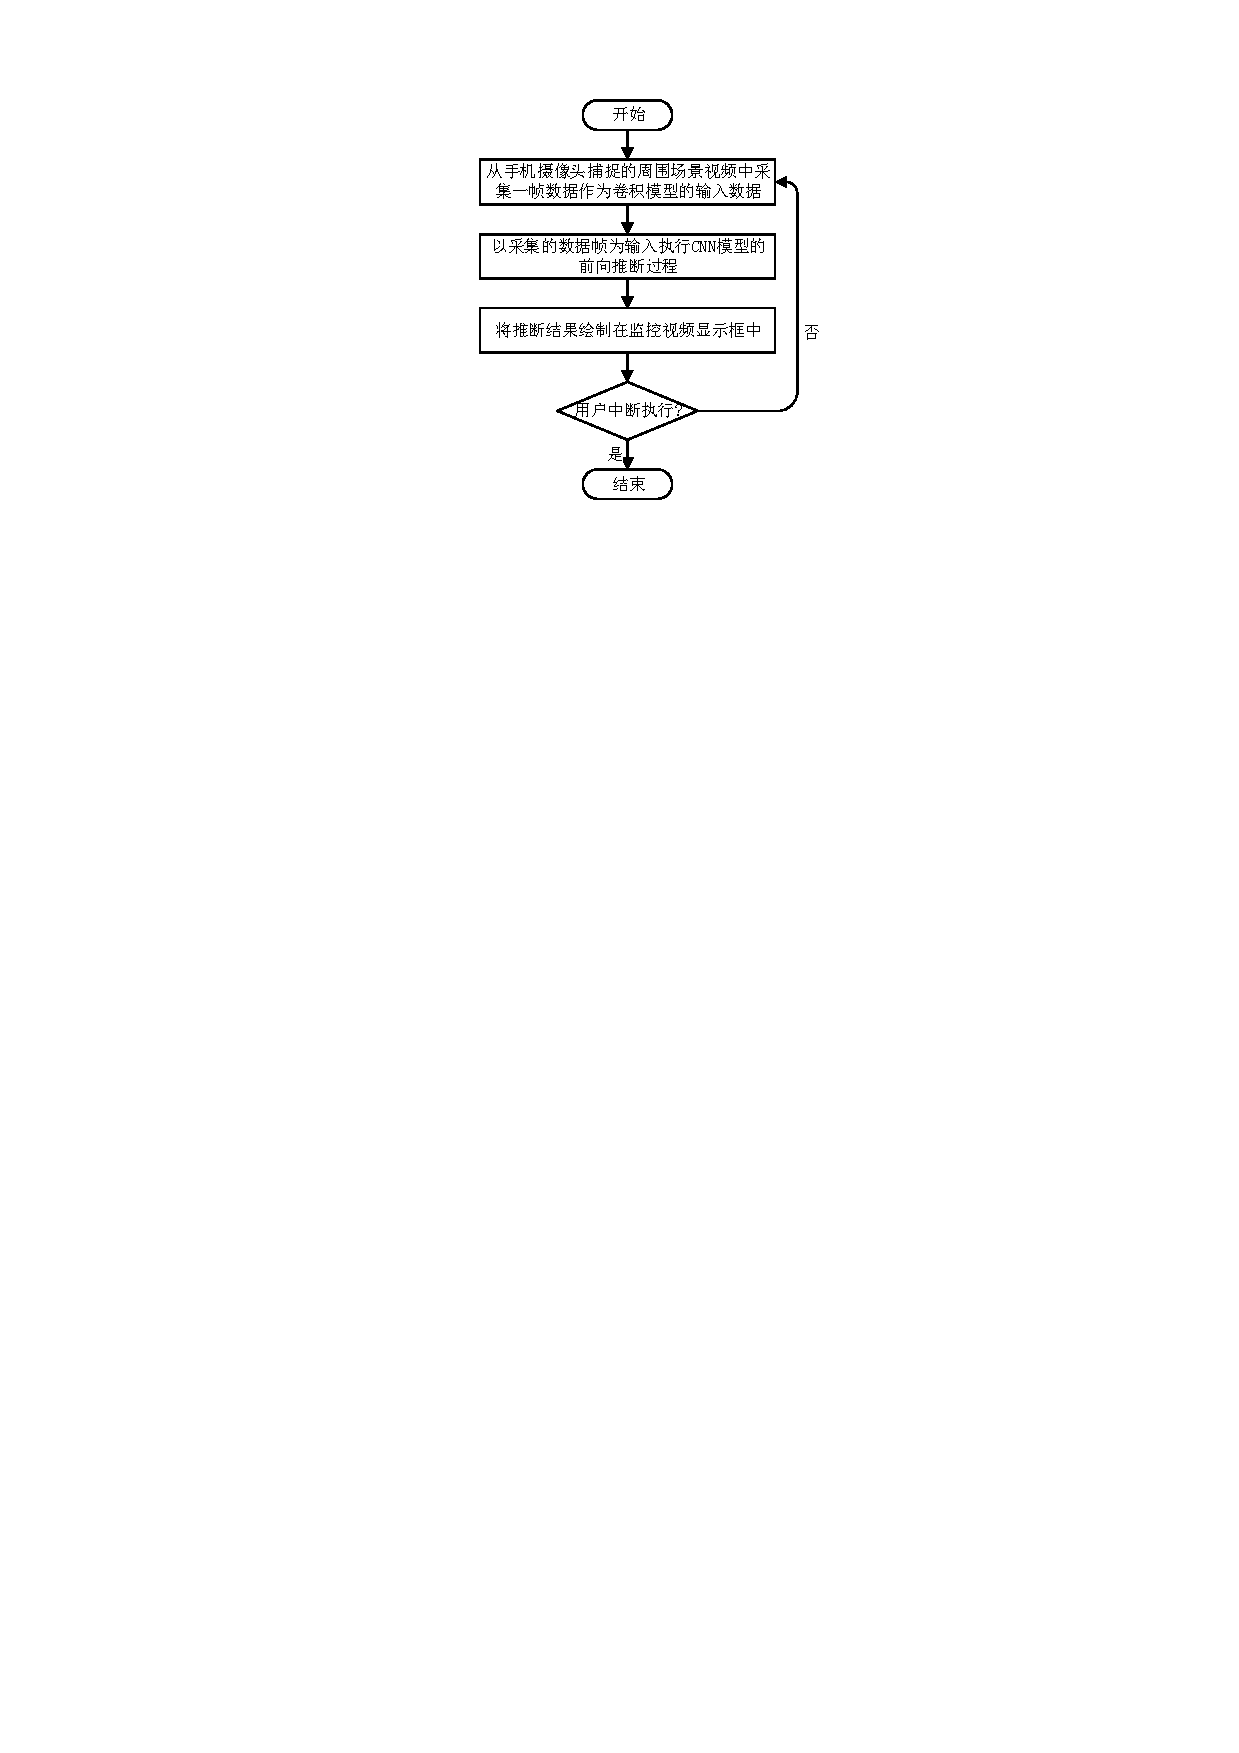
\includegraphics[height=0.5\textwidth]{figures/app_process.pdf}
    \caption{智能监控系统APP的工作流程}\label{figure:figure36}
\end{figure}

为了探索从系统层进一步优化基于CNN模型的手机应用,本文基于ODROID-XU3平台考察了智能监控系统APP的运行时负载特征。由第\ref{chapter:chapter4}章可知,智能监控系统APP在ODROID-XU3上主要使用GPU执行CNN的前向推断过程,故而可使用GPU的利用率作为该APP的负载。图\ref{figure:figure37}显示了在Android系统GPU默认功耗管理策略下智能监控系统APP的负载和GPU频率变化情况。
由图\ref{figure:figure37}可以看出,智能监控系统APP对GPU的利用率平均值为86.59\%,并且绝大多数的利用率值都在平均线以上。智能监控系统APP的负载曲线形状类似了周期脉冲图,这与该APP的实际工作流程相符合。因为智能监控系统APP的工作流程就是周期性的“采样-推断-绘制”。由智能监控系统APP的负载曲线上只有一个很窄的峰谷可知,“采样-推断-绘制”操作中推断占了整个APP运行时间的绝大部分。
\begin{figure}[htbp]
    \centering
    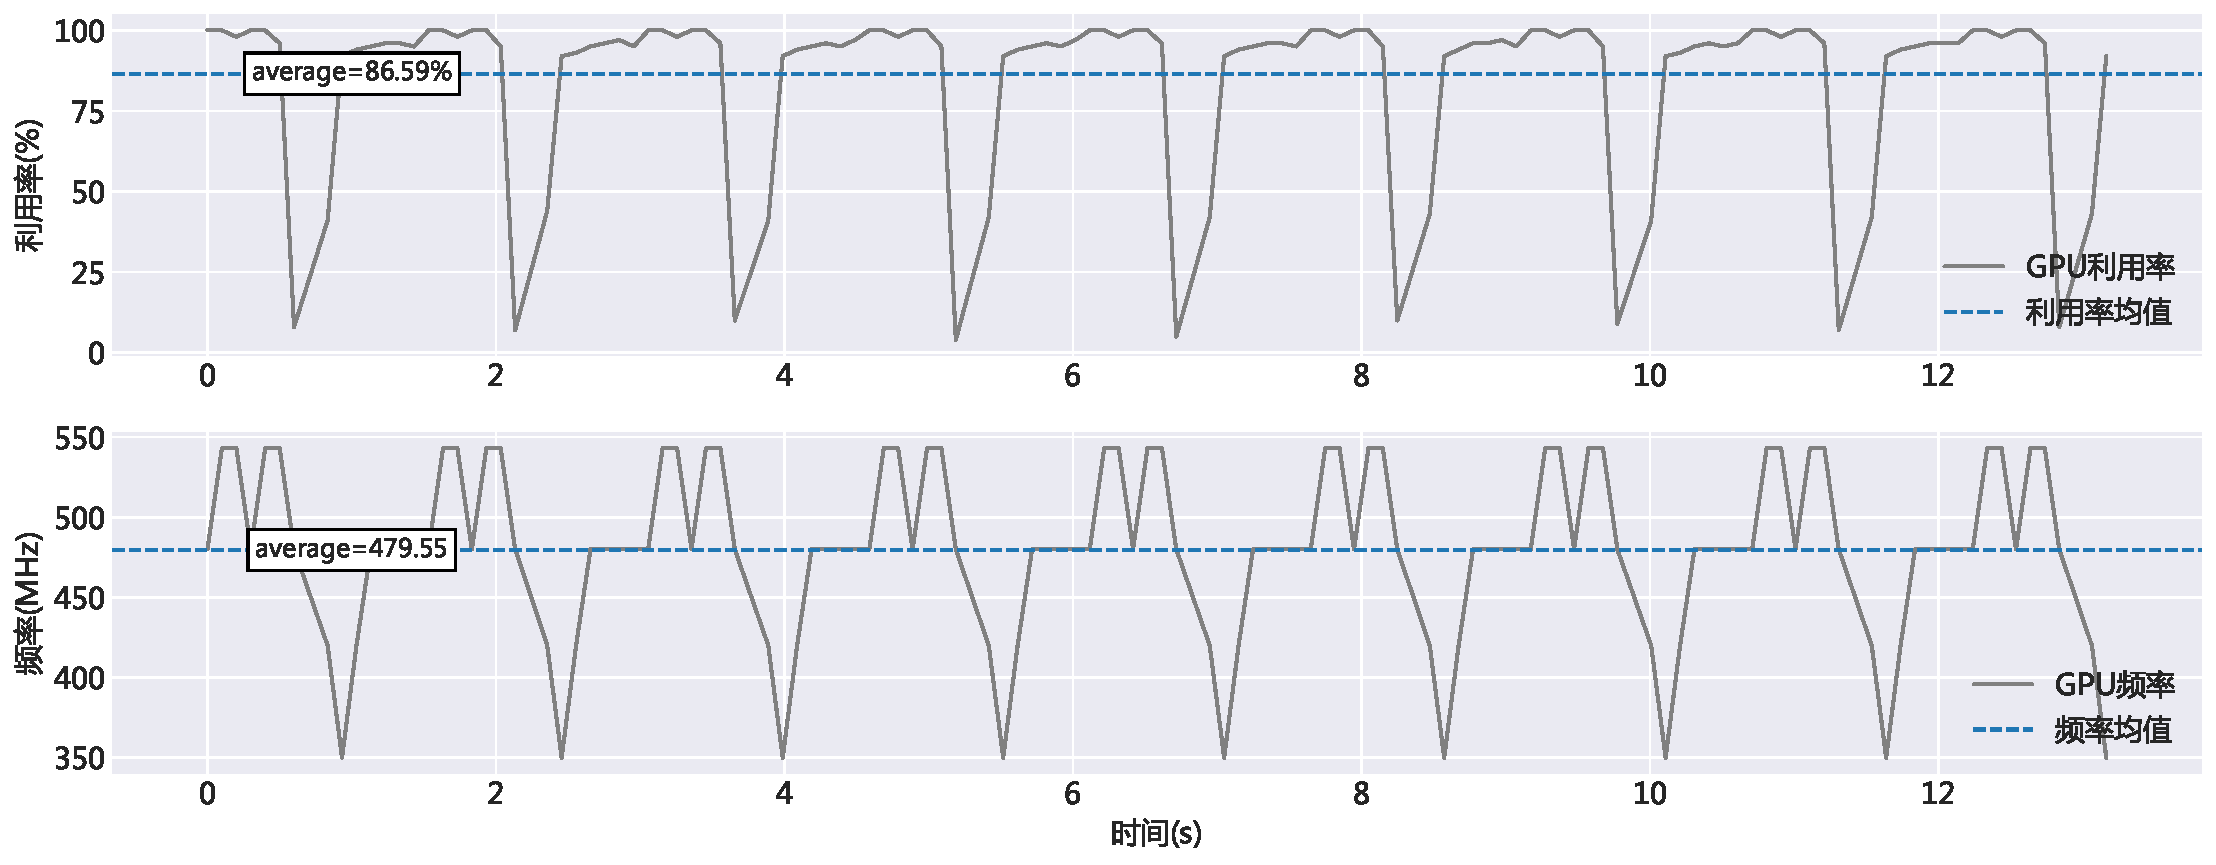
\includegraphics[width=1.0\textwidth]{figures/system_util.pdf}
    \caption{智能监控系统APP的负载和GPU频率变化}\label{figure:figure37}
\end{figure}




\section{基于应用场景的系统层能效优化策略}
\label{chapter5-3}

\section{本章小结}


\cleardoublepage
\chapter{总结与展望}

\section{本文工作总结}
当今社会,移动手机已然成为人类生活中不可或缺的贴身物品,并且用户对其智能化程度要求也越来越高。为此,许多手机生产商将人工智能技术应用于手机平台,借以为使用者提供更加人性化的服务,如苹果iPhone X、华为 Mate 10系列等。卷积神经网络(CNNs)是人工智能领域中一种成熟的神经网络模型,其已经被应用于手机平台为人类解决生活中遇到的诸多问题,如人脸识别、机器翻译等。为了更好地保障手机用户的隐私并避免网络性能的不稳定,基于人工智能模型的手机应用愈来愈偏向于使用手机本地端设备处理器完成前向推断过程而非上传到云端服务器执行。本文针对CNN模型于Android手机平台进行离线推断的过程提出了一系列能效优化策略,主要工作包括如下:
\begin{enumerate}
  \item 基于OpenCL异构编程框架开发了一套可在手机GPU上执行CNN前向推断的运行时库。利用该套CNN推断时库,本文在手机移动平台上分别重构了LeNet-5模型和AlexNet模型。实验发现,LeNet-5模型在手机GPU上进行前向推断的执行速度是其在手机CPU上的11倍以上,并且可以节省120多倍的能耗。而对于AlexNet这种复杂度较高的模型,其在手机GPU上执行前向推断相较于手机CPU而言性能加速比可达15,而GPU推断能耗也仅为CPU推断能耗的1/30。
  \item 基于“剪枝-重训”的模型压缩方法对卷积神经网络中占存储量主要部分的全连接层权重进行压缩,并在CNN推断时库中引入稀疏矩阵向量乘(SpMV)使得推断时库支持经压缩处理的稀疏CNN模型。实验证明,对网络模型进行压缩不仅可以降低手机内存占用、提高模型加载速度,还可以在一定程度上加速模型于移动端的推断过程。
  \item 结合移动端SoC架构的发展趋势,本文提出了一种基于手机平台异构设备处理器高能效并行执行CNN推断的优化策略。该策略使得CNN推断时库在运行中可自动感知目标平台上不同异构设备处理器的推断能效,并根据这些能效差异自适应找到一个可高能效执行CNN推断的设备处理器组合。实验结果发现,与总是试图使用所有可获得异构设备处理器的贪心策略相比,本文所提出的策略可以获得3.67倍更高的能效且仅仅损失9.7\%的执行速度。
  \item 通过分析智能监控系统Android应用这种基于CNN模型生活日志型APP的系统层负载特征,本文发现系统默认使用的GPU调频策略会产生“乒乓效应”并造成额外的能耗开销,而将GPU频率固定在最大可达频率点CNN推断性能更高且几乎不影响推断能效。因此,本文提出了一种基于应用场景的GPU调频策略,其可自动感知系统上层应用是否为基于CNN模型的生活日志型应用,并根据检测结果及时改变调频行为。
\end{enumerate}


\section{未来工作展望}
本文针对基于CNN模型的手机应用如何在移动平台上高能效执行这一研究问题,提出了一系列能效优化策略,包括结合模型压缩的手机GPU加速推断、使用异构设备处理器并行推断以及根据应用场景的特点进行系统层优化等。然而,为了使CNN模型广泛地应用于商业手机平台,在本文研究内容的基础上仍然存在着许多待优化的工作。

首先,本文实验发现,手机平台的访存速度普遍较低,所以模型体积较大时其推断速度受访存影响较为明显。在以后的研究工作中,针对手机GPU上的CNN前向推断过程,可以使用半浮点型数据代替浮点型数据。虽然这种做法可能会造成些许的推断精度损失,但是其不仅能够降低内存占用和访存能耗还可以在一定程度上提高推断执行速度。另外,若手机GPU存在着本地内存(local memory),应尽量使用本地内存代替全局内存以加快访存速度。本文研究工作仅压缩了卷积模型中占存储量主要部分的全连接层权重,而未来将会对卷积层权重进行压缩并探索为压缩后的卷积层提供移动端运行支持的方法。

其次,本文提出的基于异构设备处理器高能效并行执行CNN推断的优化策略中没有考虑任务划分所导致的数据通信开销,这将被加入到未来的研究工作计划中。另外,研究中仅按输出节点对单层的计算任务进行划分,在今后的研究工作中将进一步探索更细粒度的计算任务划分方法。

最后,本文对CNN模型推断在系统层进行能效优化的探索是初步的,它为以后的研究工作提供了手机系统层优化CNN推断的思路。针对基于CNN模型的手机应用,未来的工作将探索更加通用、智能的系统功耗管理器。
\cleardoublepage 
\bibliography{bib/ustc}
\cleardoublepage 

%\appendix
%\chapter{论文规范}

\backmatter
\begin{acknowledgements}
时光荏苒,三年的研究生学习生涯已悄然接近尾声。三年前的我追随自己内心的兴趣所在毅然选择从其他专业跨入到计算机科学这个领域,三年后的我依然不后悔当初的选择。这三年来,我完成了从对科研的陌生、迷茫到乐在其中的蜕变。期间,我收获到的不仅仅是知识还有道不尽的友情、师生情,而我需要感谢的人也有很多。

首先,我很庆幸三年的学习生活中有着四位导师对我悉心教导。感谢周学海老师,是他将我带入了计算机领域科学研究的大门。周老师为人和蔼可亲,很少见到他发脾气,但是当我们科研不努力时他也会恨铁不成钢地批评我们。正是因为周老师对学生的严格要求,我学会了主动阅读与自己研究工作相关的论文、认真解决科研中遇到的问题。感谢李曦老师,是他每次在我研究工作遇到瓶颈停滞不前时,及时给予我解决问题的思路。李老师对于科研工作一丝不苟的态度一直是我学习的榜样。虽然李老师平时表现得严厉,但是他其实也很幽默,对待学生更是关爱有加。感谢王超老师在研究工作和论文书写上给我提出的建议。超哥每次对我科研工作的点评都是一针见血,让我及时意识到研究过程中存在的问题。感谢陈香兰老师在科研和学习生活上对我的帮助。在科研或生活上遇到解不开的难题时,陈老师的一番话总能让我恍然大悟,给予我思路和信心去战胜困难。

其次,我要感谢程志南师兄、宋家臣师兄、周金红师兄、徐友军师兄以及赵洋洋师姐。程志南师兄是我在研究生学习生涯中遇到的贵人。从开题选择到小论文写作,对于我每次的叨扰,南哥都会很有耐心地和我讨论,给我指明方向。感谢宋家臣师兄深夜还在和我探讨我的开题工作,他有条不紊的做事风格十分值得我学习。感谢周金红师兄在我研究生选题时给予我的一些建设性意见。感谢徐友军师兄带领我学习Linux内核,为我以后的科研工作打下了技术基础。感谢赵洋洋师姐给予我科研问题上的一些解决思路。当然,我还要感谢我的同窗好友张奕玮、罗海钊、徐冲冲、孙凡、鲁云涛、郭玲等人,是他们陪我度过了整个研究生学习生活,是他们在我遇到困难时给予我鼓励,是他们让我在科研道路上走得更远。

最后,我要感谢我的爸爸和妈妈。他们虽然都年过半百,但是对于我的求学之路总是无条件支持。我很愧对我的父母,五十几岁本该是他们安享晚年的年龄,但是因为我还在读书,他们仍在不辞劳苦地工作着。祝愿我的父母身体健康,希望我所学之知识能够报答他们的养育之恩。

\begin{flushright}
王震 \\
于2018年4月
\end{flushright}



\end{acknowledgements}

\cleardoublepage 
\begin{publications}

\section*{已发表论文}

\begin{enumerate}
\item Zhen Wang, Xi Li, Chao Wang, Zhinan Cheng, Jiachen Song, and Xuehai Zhou.\\
Rethinking Energy-Efficiency of Heterogeneous Computing for CNN-Based Mobile Applications[C]//
15th IEEE International Symposium on Parallel and Distributed Processing with Applications(IEEE ISPA 2017)
\item Zhen Wang, Zhinan Cheng, Xi Li, Chao Wang, Xianglan Chen, and Xuehai Zhou.\\
Building A Game Benchmark for Cooperative CPU-GPU with Pseudo User-interaction[C]//
15th IEEE International Symposium on Parallel and Distributed Processing with Applications(IEEE ISPA 2017)
\end{enumerate}


\section*{参与的主要项目}
\begin{enumerate}
\item 科技委前沿创新计划项目——智能计算机
\end{enumerate}

\end{publications}

\cleardoublepage 

\end{document}
